\documentclass[11pt]{ucthesis}
\setlength{\oddsidemargin}{0.15in}
\def\dsp{\def\baselinestretch{1.75}\large\normalsize}
\ssp

\usepackage{amsmath}
\usepackage[pdftex]{graphicx}
\usepackage{times}
\usepackage{amsfonts}
\usepackage[usenames,dvipsnames]{color}
\usepackage{verbatim}
\usepackage{fancyvrb, relsize}
\usepackage{url}
\usepackage{hyperref}
\usepackage{wrapfig}
\usepackage{subfigure}
\usepackage{multirow}
\usepackage{algorithm2e}
\usepackage{listings}


\lstdefinelanguage{pret}
{morekeywords={get_time, delay_until, delay_and_set, exception_on_expire, deactivate_exception}}

\lstset{frame=shadowbox, numbers=right, basicstyle=\footnotesize, keywordstyle=\textbf, language=pret}

\newcommand{\gettime}{\textbf{get\_time}}
\newcommand{\delayuntil}{\textbf{delay\_until}}
\newcommand{\delayandset}{\textbf{delay\_and\_set}}
\newcommand{\exceptiononexpire}{\textbf{exception\_on\_expire}}
\newcommand{\deactivateexception}{\textbf{deactivate\_exception}}
\newcommand{\mtfd}{\textbf{mtfd}}

\newcommand{\Gettime}{\textbf{Get\_time}}
\newcommand{\Delayuntil}{\textbf{Delay\_until}}
\newcommand{\Delayandset}{\textbf{Delay\_and\_set}}
\newcommand{\Exceptiononexpire}{\textbf{Exception\_on\_expire}}
\newcommand{\Deactivateexception}{\textbf{Deactivate\_exception}}


\newcommand{\rt}{real-time}
\newcommand{\Rt}{Real-time}
\newcommand{\thdint}{thread-interleaved}
\newcommand{\Thdint}{Thread-interleaved}
\newcommand{\todo}[1]{{{\textcolor{Red}{(Todo: #1)}}}}%
\newcommand{\mycaption}[1]{\vspace{-7mm}
\caption{#1}
\vspace{-4mm}}
\newcommand{\hpstar}[2]{#1}

\newcommand{\IL}[1]{{{\textcolor{Blue}{(IL: #1)}}}}
\newcommand{\HP}[1]{{{\textcolor{Purple}{(HP: #1)}}}}
\newcommand{\JR}[1]{{{\textcolor{Green}{(JR: #1)}}}}
\newcommand{\EAL}[1]{{{\textcolor{Red}{(EAL: #1)}}}}

%\renewcommand*\thesubsection{\thesection.\roman{subsection}}
\renewcommand*\thesubsubsection{\thesubsection.\alph{subsubsection}}

\begin{document}
\title{Precision Timed Machines
\iffalse
From Ptides to PtidyOS, Designing Distributed Real-Time Embedded Systems
  \titlenote{This work was supported in part by the Center for Hybrid and Embedded Software Systems (CHESS) at UC Berkeley, which receives support from the National Science Foundation (NSF awards \#0720882 (CSR-EHS: PRET), \#0931843 (ActionWebs), and \#1035672 (CSR-)CPS Ptides)), the U. S. Army Research Office (ARO \#W911NF-07-2-0019), the U. S. Air Force Office of Scientific Research (MURI \#FA9550-06-0312), the Air Force Research Lab (AFRL), the Multiscale Systems Center (MuSyC), one of six research centers funded under the Focus Center Research Program, a Semiconductor Research Corporation program, and the following companies: Bosch, National Instruments, Thales, and Toyota.}
\fi
}
\author{Isaac Liu} 
\degreeyear{2012}
\degreesemester{Spring}
\degree{Doctor of Philosophy}
\chair{Professor Edward A. Lee}
\othermembers{Professor John Wawrzynek \\
Professor Alice Agogino}
\numberofmembers{3}
\prevdegrees{Bachelor of Science (University of California, Santa Barbara) 2007}
\field{Electrical Engineering and Computer Science}
\campus{Berkeley}

\maketitle
%FIXME for the final version, comment out the approval page.
\approvalpage
\copyrightpage

\begin{abstract}
Cyber-Physical Systems (CPS) are integrations of computation with physical processes~\cite{Lee08_CyberPhysicalSystemsDesignChallenges}.
%A number of applications can benefit from the potential of CPS. 
These systems must be equipped to handle the inherent concurrency and inexorable passage of time of physical processes.  
Traditional computing abstractions only concern themselves with the �functional� aspects of a program, and not its timing properties.
Thus, nearly every abstraction layer has failed to incorporate \emph{time} into its semantics; the passage of time is merely a consequence of the implementation. 
When the temporal properties of the system must be guaranteed, designers must reach beneath the abstraction layers.
This not only increases the design complexity and effort, but the systems are overdesigned, brittle and extremely sensitive to change.

In this work, we address the difficulties of handling \emph{time} in computing systems by re-examining the lower levels of abstraction. 
In particular, we focus on the instruction set architecture (ISA) layer and its affects on microarchitecture design.
The ISA defines the contract between software instructions and hardware implementations. 
Modern ISAs do not constrain timing properties of instructions as part of the contract. 
Thus, architecture designs have largely implemented techniques that improve average performance at the expense of execution time variability.
This leads to imprecise WCET bounds that limit the timing predictability and timing composability of architectures.  

In order to address the lack of temporal semantics in the ISA, we propose instruction extensions to the ISA that give temporal meaning to the program. 
The instruction extensions allow programs to specify execution time properties in software that must be observed for any \emph{correct} execution of the program.
These include the ability to specify a minimum execution time for code blocks, and the ability to detect and handle missed deadlines from code blocks that exhibit variable execution times.
This brings control over timing to the software and allows programs to contain timing properties that are independent of the underlying architecture.   
In addition, we present the Precision Timed ARM (PTARM) architecture, a realization of Precision Timed (PRET) machines~\cite{edwards2007case} that provides timing predictability and composability without sacrificing performance. 
PTARM employs a predictable thread-interleaved pipeline with an exposed memory hierarchy that uses scratchpads and a predictable DRAM controller. 
This removes timing interference among the hardware threads, enabling timing composability in the architecture, and provides deterministic execution times for instructions within the architecture, enabling timing predictability in the architecture.  
We show that the predictable thread-interleaved pipeline and DRAM controller design also achieve better throughput compared to conventional architectures when fully utilized, accomplishing our goal to provide both predictability and performance.  

To show the applicability of the architecture, we present two applications implemented with the PRET architecture that utilize the predictable execution time and the extended ISA to achieve their design requirements. 
The first application is a real-time fuel rail simulator that implements a one dimensional computational fluid dynamics (1D-CFD) solver on a multicore PRET architecture.
The implementation leverages the timing instructions to synchronize the communication of multiple PRET cores with low overhead. 
The predictable nature and the improved throughput of the architecture allow us to optimize the resource usage while statically ensuring that the timing requirements are met.
This provides a scalable solution to close the loop of fuel delivery, allowing for more precise fuel injections that lead to a cleaner and more efficient engine.
The second application presents a case study that uses PRET to remove the vulnerability of timing side-channel attacks on encryption algorithms.
Encryption algorithms are vulnerable to side-channel attacks that measure the execution time of the encryption to derive the encryption key. 
The uncontrollable execution time variance can stem from the unpredictable sharing of architecture features or from the various control paths of the encryption algorithm. 
We implement the RSA and DSA~\cite{dss} encryption algorithms on PRET and show that by using the timing extended ISA and a predictable architecture, we can completely remove the vulnerabilities that are exploited for the attacks.

By providing a predictable architecture, we provide simpler and more accurate timing analysis of the software.  
With the instruction extensions to the ISA, we provide timing control and allow architecture independent timing properties to be specified in the software. 
Through these contributions, we aim to introduce a timing deterministic foundation to the lower levels of computing abstractions, which enables more precise and efficient control over timing for the design of CPS.



\end{abstract}

\begin{frontmatter}

\begin{dedication}
\null\vfil
{\large
\begin{center}
%\\\vspace{12pt}
To my wife Emily Cheung, my parents Char-Shine Liu and Shu-Jen Liu, and everyone else whom
I've had the privilege of running into for the first twenty-seven years of my
life.
%\\\vspace{12pt}
\end{center}}
\vfil\null
\end{dedication}

\tableofcontents
\listoffigures
\listoftables
\begin{acknowledgements}

I want to thank my wife

I want to thank my parents

I want to thank my advisor, Edward A. Lee

I want to thank the committee members

I want to thank all that worked on the PRET project with me: 

Ben Lickly

Hiren Patel

Jan Rieneke

Sungjun Kim

David Broman

I would also like to thank the ptolemy group especially Christopher and Mary, Jia for providing me the template

I would like to thank everyone else that made this possible

\end{acknowledgements}

\end{frontmatter}

\chapter{Introduction}
\label{chapter:intro}
%Cyber physical systems - different than traditional embedded systems that interact with real world. Timing requirements, but large, and safety critical
\section{Motivation}
\emph{Cyber-Physical Systems} (CPS) are integrations of computation with physical processes~\cite{Lee08_CyberPhysicalSystemsDesignChallenges}.
In these systems, computation and physical process often form a tight feedback loop, affecting the behavior of each other.
The embedded platforms and networks employed not only control the physical process, but at the same time monitor and adapt to the changes of the physical process.
An enormous number of applications can be categorized as CPS.
They include high confidence medical devices and systems, assisted living, traffic control and safety, advanced automotive systems, process control, energy conservation, environmental control, avionics, instrumentation, critical infrastructure control (electric power, water resources, and communications systems for example), distributed robotics (telepresence, telemedicine), defense systems, manufacturing, and smart structures.
However, in order for CPS to be deployed in high confidence systems, such as advanced automotive or avionics systems, the platforms employed need to deal with two important properties of the physical process: they are inherently concurrent, and time progresses at its own pace.
 
%modern design techniques are hitting a scalability wall - RTOS, compilers, general purpose architectures all create problems
%all layers need work. Modern abstraction layers omit time.. designers need to reach down below, can't certify a system with its hardware
% We deal with the ISA and architecture design

Traditionally, real-time embedded systems have dealt with the notion of time.
These systems impose deadlines and timing constraints to their underlying tasks to deliver services in real time. 
The timing constraints of \emph{soft real-time systems} are typically used to guarantee quality of service, while the constraints of \emph{hard real-time systems} are used to guarantee safety critical tasks, so they must be met. 
The real-time embedded community has widely adopted techniques developed for general purpose applications, believing that they will provide the same advantages and benefits for embedded systems.
These include the programing language, the operating system, the tool-chains, and the computer architecture.
However, these techniques are designed for general purpose systems that do not require stringent interaction with the physical environment. 
Thus, they place emphasis on improving average performance over predictability.   
As a result, when computing systems absolutely must meet tight timing constraints, these computing advances often do more harm than good~\cite{LeeOnTime2005}.
%this is contrary to reality~\cite{halang:DSP:2004:4,thiele:04:predictable}.
The scale and complexity of traditional embedded systems allow designers to compensate with extra effort in design and analysis. 
However, these solutions begin to break down when transitioning to larger scale CPS.   

In the current state of embedded software, nearly every abstraction has abstracted away \emph{time}.
The Instruction Set Architecture (ISA), meant to hide the hardware implementation details from the software, does not include timing semantics for the instruction executions.  
Widely adopted programming languages, meant to hide the details of the ISA from the program logic, do not express timing properties; timing is merely an accident of the implementation.
Real-time operating systems (RTOS), meant to hide the details of the program from their concurrent orchestration, often use priorities to dictate the execution of tasks; the execution time of tasks can easily affect the scheduled outcome of execution.
The lack of \emph{time} in the abstraction layers can lead to the following consequences:
\begin{itemize}
\item \emph{Unnecessary complexities in the interaction of concurrent components} --  
This often is manifested when components share resources. 
For example, software threads are the typical abstractions for concurrent software written in C or Java. 
Because there is no guarantee of when a shared variable will be accessed by each thread, locks and semaphores are required to avoid race conditions. 
This not only introduces bugs, but also introduces complex and almost impossible to analyze interactions between threads~\cite{leethreads}. 
As a result, there is great difficulty when synchronizing and communicating between components or tasks.

\item \emph{Unnecessary complexities in interactions across layers} -- 
For example, scheduling could be done at multiple levels simultaneously without any coordination. 
As tasks or software threads are scheduled for execution in the OS, an explicit multithreaded dynamic dispatch architecture could also be scheduling instructions from different hardware threads without the knowledge of the OS~\cite{thiele:04:predictable}.

\item \emph{Misleading or pessimistic analysis results when analyzing the whole system} -- 
For example, task scheduling and context switching cost may vary from the cache or pipeline state change after executing each tasks. 
This is often not factored into the analysis~\cite{thiele:04:predictable}. 
Furthermore, because the  large variation of execution time in modern complex processors, worst-case execution time (WCET) analysis techniques often lead to overly conservative results for safety~\cite{wilhelm-survey-paper}. 
As the WCET is often the basis for priority of any scheduling scheme, the conservativeness is propagated throughout the system.
\end{itemize}
%explain composability

When the temporal properties of the system must be guaranteed, designers must reach beneath the abstraction layers, and understand thoroughly the complex underlying details and its affect on execution time. 
This not only increases the design complexity and effort, but the designed systems are \emph{brittle} and extremely sensitive to change~\cite{Sangiovanni-Vincentelli2007automotive, edwards2007case}.  
For example, Sangiovanni-Vincentelli et al.\cite{Sangiovanni-Vincentelli2007automotive} show that when increasing the execution time of a task, any priority based scheduling scheme results in discontinuity in the timing of all tasks besides the task with the highest priority. 
At a lower level, adding a few instructions can easily result in a huge variation in program execution time; the state of the hardware dynamic prediction and speculation units, such as caches and pipelines, can easily be affected by small program additions.
Thus, in order to verify the timing of safety critical systems, the verification must be done on both the software system and its execution platform; they cannot be separated. 
This process is often time consuming and expensive.
Since the abstraction layers do not give any temporal semantics to the system, each layer must be completely understood in order to reason about and prove the timing properties of the full system.  
For avionics manufacturers, this means stockpiling the same hardware for the lifetime of an aircraft; any upgrade of components or software in their system could result in drastic timing changes, and thus require re-certification.


\subsection{Timing Predictable Systems}
Thiele et al.~\cite{thiele:04:predictable}, Henzinger~\cite{Henzinger2008} and Lee~\cite{LeeOnTime2005} have all identified the importance and difficulties of designing \emph{timing-predictable systems}.
Timing-predictable systems should exhibit the following property: \textit{a small change in the input must not result in a large change in the output}~\cite{Henzinger2008}.
If the definition of \emph{output} includes the timing behavior exhibited by the system, then current abstractions disrupts this property at almost all levels. 

A change is needed to efficiently and safely design next generation systems, especially if they effect the well being of our lives.
In particular, how software and hardware deal with the notion of \textit{time} needs to be more carefully understood and designed.
At the lowest levels of abstraction, circuits and microarchitectures, timing is central to correctness.
For example, in a microarchitecture, if the output of an ALU is latched at the wrong time, the ISA will not be correctly implemented.
However, at higher levels, for example, the ISA, timing is hidden, and there are no temporal semantics; the execution time is irrelevant to correctness. 
Thus, each abstraction layer needs to be revisited to judiciously introduce some form of temporal semantics. 
Specifically for CPS, platforms must be equipped to handle the \emph{inherent concurrency} and the \emph{inexorable passage of time} for physical processes.   
Sangiovanni-Vincentelli et al.~\cite{Sangiovanni-Vincentelli2007automotive} identified these issues as the \textit{timing composability} and \textit{timing predictability} of systems, and list them as requirements to enable efficient designs of large-scale safety-critical applications.    

\subsubsection{Timing Composability}
Modern systems handle the concurrency of physical processes with multiple tasks, components or subsystems that are integrated together.    
In order to efficiently design the system, these individual parts are designed and tested separately, then later integrated to form the final system. 
This modularity of design is crucial for the continued scaling and improvement of systems.      
However, if component properties may be destroyed during integration, then the components can no longer be designed and verified separately. 
\textit{Timing composability} refers to the ability to integrate components while preserving their temporal properties.

To preserve component properties during integration, modern designs often use a \textit{federated architecture}.
A federated architecture develops functions and features on physically separate platforms which are later integrated through an interconnect or system bus. 
As these features are only loosely coupled through an interconnect, interference is limited, allowing the preservation of certain properties independently verified. 
However, as the platforms are feature specific, they are often idle during run time.
In order to reduce resource consumption, there is a shift towards \textit{integrated architectures}~\cite{Obermaisser2009FedtoIMA,AvionicsWatkins2007IMA}, where multiple functions are integrated on a single, shared platform.
Several challenges exists to make the shift, but among them, it is crucial to guarantee that the timing properties are preserved during system integration.
Only then can designs continue to stay modular. 
Modern abstractions result in unnecessary complexity in the interaction of concurrent components, which leads to unpredictable interference between components. 
This hinders the ability to compose functions together on a shared resource while maintaining timing properties. 

These challenges are present not only in research, but also in industry.  
The Integrated Modular Avionics (IMA) concept~\cite{IMA} aims to replace numerous separate processors and line replaceable units (LRU) with fewer, more centralized processing units in order to significant reduce the weight and maintenance savings in new generation of commercial airliners.
AUTOSAR (AUTomotive Open System ARchitecture)\cite{autosarsite} is an architecture for automotive systems that is jointly being developed by manufacturers, suppliers and tool developers that attempts to defined standards and protocols to help modularize the design of these complex systems.
We contend that in order for these standards to be safely defined, modern layers of abstraction that have been adopted from conventional computing advances must be redefined to allow for timing predictable composition of components.  

\subsubsection{Timing Predictability}
In order to keep up with the continuous passage of time in physical processes, the system must be able to reason about its own passage of time.
\textit{Timing predictability} is the ability to predict the timing properties of the system.
Timing composition plays a big part of this when features are integrated, but even separately, it is difficult to analyze the execution time of programs.

Wilhelm et al.~\cite{wilhelm-survey-paper} describe the abundance of research and effort that has been put into bounding the WCET of programs.   
Not only is determining the worst case program flow a challenge, but the precision and usefulness of the analysis also depend on the underlying architecture~\cite{Heckmann2003processor}. 
Conventional architectures have implemented techniques that target the improvement of average case execution time (ACET) at the expense of execution time variability.    
As a result, it is extremely complex, if not impossible to obtain a precise bound of the execution time on modern architectures.
The imprecision is often propagated through the system during integration, requiring pessimistic over-provisioning to ensure timing requirements are met.     
Thus, time determinism and reduced jitter are needed for future systems to increase performance~\cite{Sangiovanni-Vincentelli2007automotive}.    

As modern layers of abstraction for computing have no notion of \emph{time}, the passage of time is a merely a consequence of the implementation.  
Therefore, existing techniques can only bound the WCET for a processor-program pair, and not the individual programs.
Time bounds from the analysis are broken even when the underlying processor is upgraded to a newer model of the same family.
Thus, the redefinition of abstraction layers must also include temporal semantics to allow reasoning of timing properties at each layer independently from the abstract layers below it.  

\section{Contributions}
The contribution of this work is to provide more precise and efficient control over the timing properties of computing systems. 
Specifically in this thesis, we focus on the lack of temporal semantics in the ISA abstraction layer, and its effects on microarchitecture design. 
The ISA defines the contract between software instructions and hardware implementations.
Any correct implementation of an ISA will yield a consistent view of the processor state (eg. the contents registers or memory) for a given program developed with that ISA.     
However, modern ISAs do not specify timing properties of the instructions as part of the contract, and the benchmarks typically used to evaluate architectures compare them by the measured average performance.   
Thus, architecture designs have largely introduced techniques that improve average performance at the expense of execution time variability, leading to imprecise WCET bounds that limit the timing predictability and timing composability of the architecture.
The key challenges we contribute to are twofold.

First, we address the difficulty of predicting execution time and integrating multiple programs on modern computer architectures by proposing a new design paradigm for computer architectures.
PREcision Timed (PRET) machines~\cite{edwards2007case} are designed with \textit{timing-predictability} as the main metric for success.
However, predictability can be easily achieved if one is willing to forgo performance; computer architectures 50 years ago were very predictable.
Thus, our contribution is to deliver both predictability and performance.    
We believe that as systems are becoming increasingly large and complex, increasing the speed of the underlying architecture through complexity will only do more harm than good.
We do not intend to reinvent computing advancements, but instead evaluate them through the lenses of predictability and composability.
In doing so, we present an architecture designed for timing-predictability without sacrificing performance.   

Second, we address the lack of temporal semantics in the ISA by exploring instruction extensions that introduce timing semantics and control into programs.
Introducing temporal semantics into any abstraction layer is a non-trivial task. 
Specifically for the ISA, over constraining the timing definitions can easily thwart architecture innovation opportunities.
Thus, we explore extensions that aim to give temporal meaning to the \emph{program}, not the individual instructions. 
These instruction extensions allow programmers to describe the passage of time within programs, and any architecture implementation of the extended ISA must abide to those descriptions. 
In doing so, we give temporal meaning to programs without limiting the innovation of architecture designs.

We contend that both contributions are essential to cyber-physical systems. 
%Our ISA extensions provide the ability to give temporal meaning to programs, but do not enforce a predictable execution of its instructions.
Without a predictable architecture, programs can exhibit unpredictable execution time variances.    
But a predictable architecture by itself does not bring temporal meaning to the programs, it merely executes them predictably.
Time will still only be a side effect of the underlying implementation.
With both the ISA extensions and the predictable architecture, we equip platforms with the ability to interact with physical processes and provide 
a solid foundation to enable precise and efficient control over the timing properties of the system.
This prevents the overdesigning of computing systems for applications that absolutely must meet timing constraints, such as CPS.            
 
% 
% We use the definition from Thiele et al.\cite{thiele:04:predictable} for predictability:
% \begin{quote}
%   \textit{Predictability}: The timing predictability of a system is
%   related to the differences between best case and lower bound on the
%   one hand and upper bound and worst case on the other. The former we
%   call best case predictability, the latter worst case
%   predictability. 
% \end{quote} and we define \textit{repeatability} as follows:
% \begin{quote}
%   \textit{Repeatability}: Every correct execution of the same sequence
%   will lead to the same state given the same inputs. Any complete
%   definition of ``inputs'' must include the timing of interrupts and
%   the time at which sensor values are polled. Any complete definition
%   of ``outputs'' must also include the timing at which actuations in the
%   physical environment are asserted\cite{Edwards_adisruptive}
%   \textcolor{red}{(Repeatability needs a more clear definition)}.
% \end{quote} 

\section{Background}
\label{bookmark:timing_anomalies}
% \begin{itemize}
%   \item Discuss the problem
%   \item show the difficulty in execution time analysis of a simple c code
%   \item show the variability different architecture improvements have introduced to improve average case execution time (Sami's graph)
%   \item not saying WCET is useless, just saying that with more precise architecture designs, WCET can be more precise, less program variation
% \end{itemize}

Programs manifest varying execution times.
This is illustrated in figure~\ref{fig:program_execution_times}, which shows the distribution of execution times exhibited by an arbitrary program on an arbitrary processor.
\begin{figure}[b]
  \begin{center}
    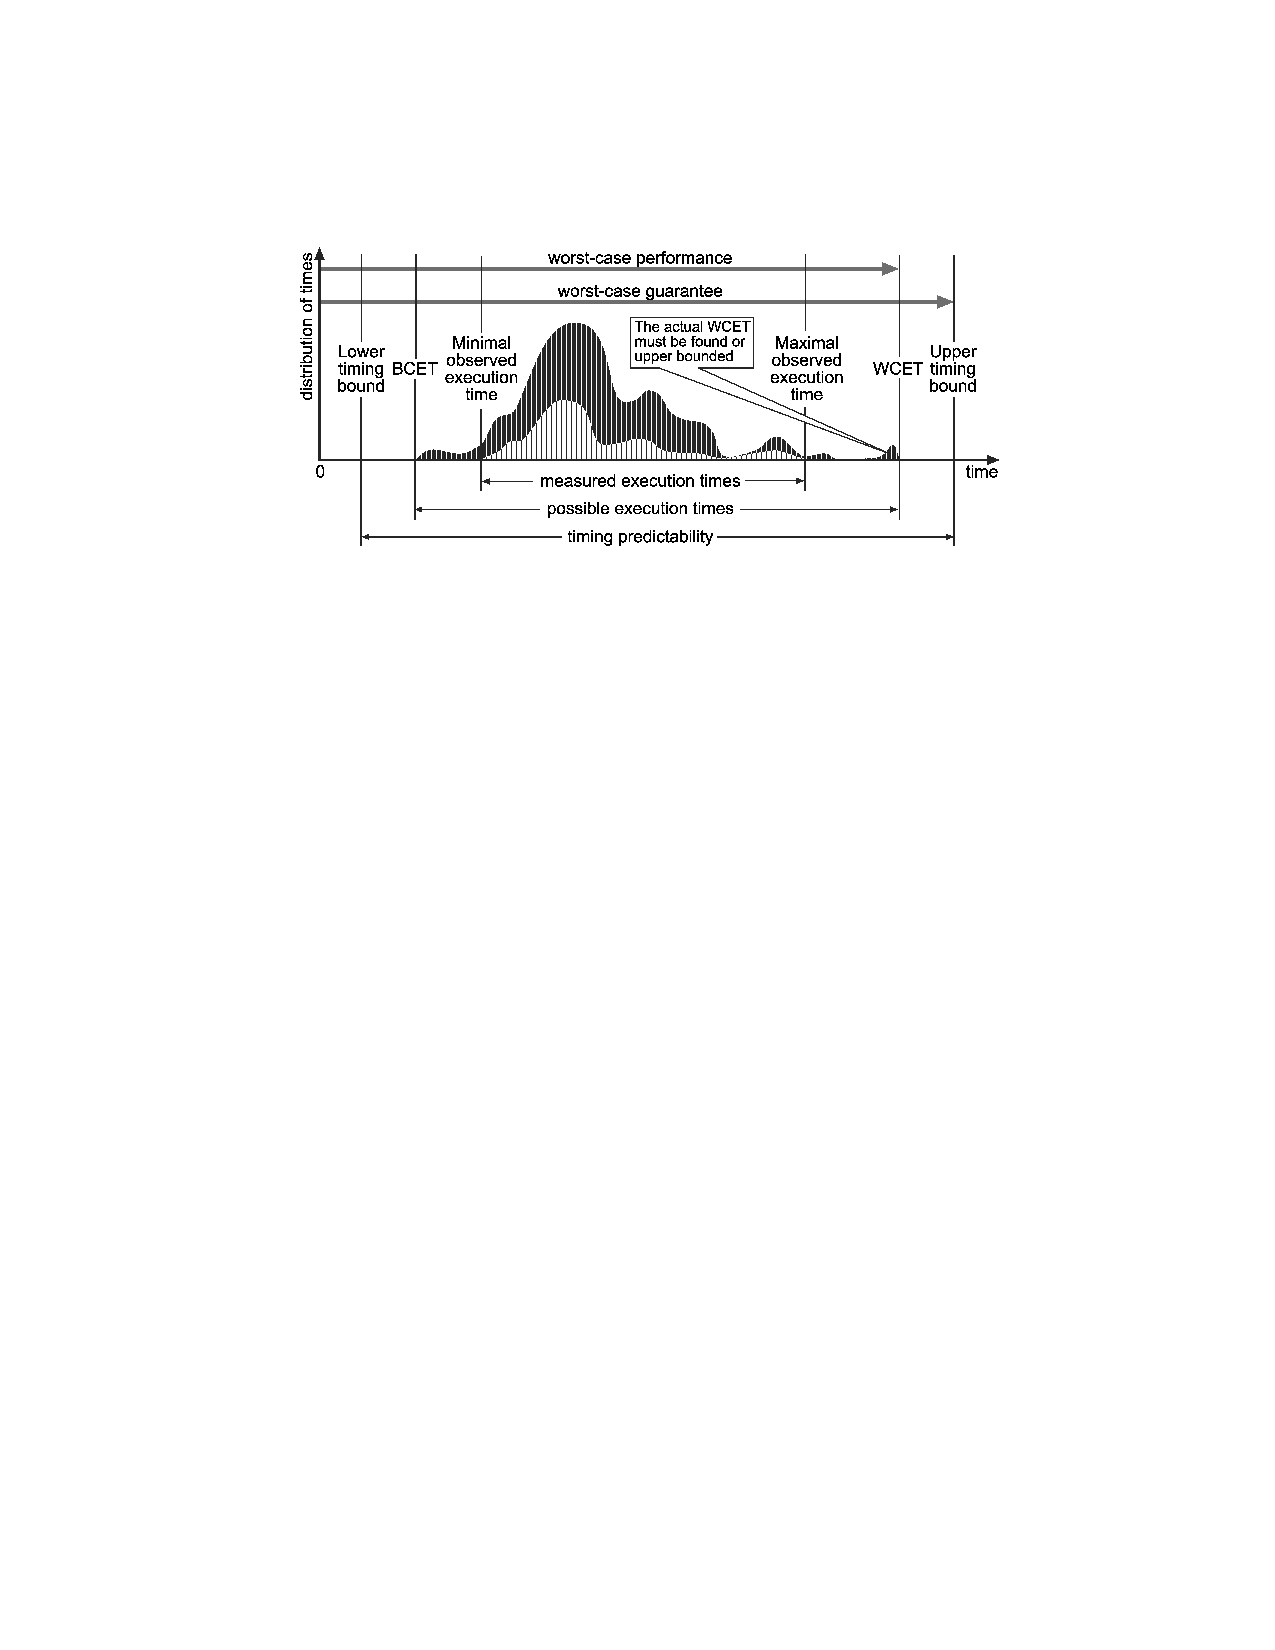
\includegraphics{figs/program_executiontimes.pdf}
  \end{center}
  \vspace{-3mm}
  \caption{``Program Execution Times~\cite{wilhelm-survey-paper}''}
  \label{fig:program_execution_times}
\end{figure}
It highlights several key issues that are important to understanding program execution time.
First, the \emph{observable execution times} may not observe all \emph{possible execution times}.
This is important because far too often we rely on testing and end-to-end measurement to determine the WCET.
This will, in general, overestimate the best-case execution time (BCET) and underestimate the WCET, and is not safe when timing must be guaranteed. 
Second, it is often difficult to determine the \emph{actual} WCET, thus the worst case guarantee that is given is usually a bound on the WCET.    
The goal of the WCET analysis is to obtain a \textit{safe} and \textit{precise} bound on the WCET of a program~\cite{wilhelm-survey-paper}. 
\textit{Safe} means that the execution time will never exceed the bounded time. 
\textit{Precise} means that the bounded time is as close to the absolute WCET as possible. 

Several factors contribute to the difficulties of a safe and precise WCET analysis.
In general, it is impossible to obtain the upper bounds on execution times for programs because programs are not guaranteed to terminate.  
Real-time systems use a restricted form of programming to ensure an execution time upper bound.
Recursion is often not allowed or must be explicitly bounded, as are the iteration counts of loops. 
Despite that, algorithms contain input dependent program paths that complicate analysis.    
The worst case program path depends on the worst-case input, which in general, is not known or hard to derive.    

Along with complications from the software structure, the execution time variance exhibited by the underlying architecture further complicates analysis.   
A conventional microprocessor executes a sequence of instructions from an instruction set. 
Each instruction in the instruction set changes the state of the processor in a well-defined way.
The microprocessor provides a strong guarantee about this behavior: a sequence of instructions \emph{always} changes the processor state in the sequential order of the instructions.        
For speed, however, modern microprocessors rarely execute the instructions strictly in sequence. 
Instead, pipelines, caches, write buffers, and out-of-order execution reorder and overlap operations while preserving the illusion of sequential execution.  
This causes the execution time of even the same sequence of instructions to fluctuate, depending on the architecture's underlying execution of its instructions.
To illustrate this, we show in figure~\ref{fig:simple_code_timing_issues} a code segment with a simple control structure and a static loop bound.

%predictability -   
  % C code example
  % modern architecture improvements
\begin{wrapfigure}{r}{0.45\textwidth}
  \vspace{-20pt}
  \begin{center}
    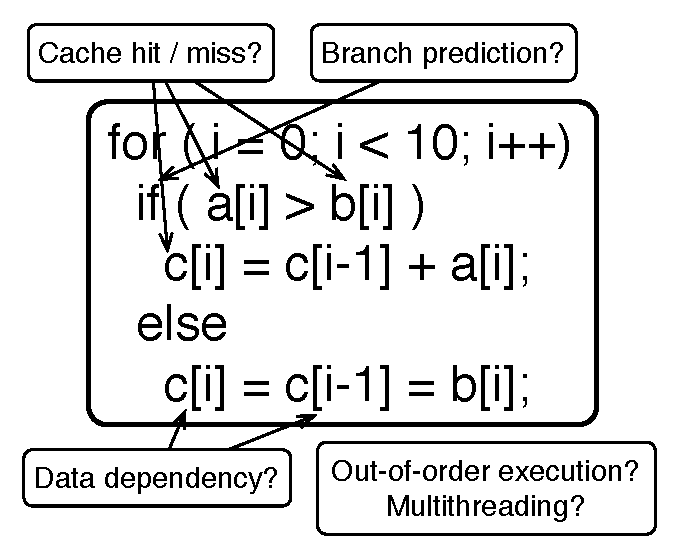
\includegraphics[scale=.6]{figs/simple_code_timing_issues}
  \end{center}
  \vspace{-10pt}
  \caption{Simple Loop Timing Issues}
  \label{fig:simple_code_timing_issues}
  \vspace{-10pt}
\end{wrapfigure}

Even with a simple software structure, several situations can arise from the execution on the underlying architecture. 
Each array access in the code is compiled into a memory access.
Whether the memory access hits or misses the cache has huge implications on program execution time.
The \emph{if} statement is usually compiled to a conditional branch.
The outcome of the branch predictor could easily affect the execution time of the program.
%Furthermore, the speculatively executed instructions could modify the cache state which can cause future memory accesses to delay.        
Superscalar architectures can execute instructions out-of-order, so data-dependencies in this code may or may not stall, depending on the memory accesses and how much loop unrolling is done by the compiler/architecture.   

Further complications arise as architectures become increasingly parallel with multiprocessing techniques such as multicore and multithreading.
These techniques allow the architecture to inherently handle concurrency, but can easily introduce temporal interference even between logically independent behaviors.
For example, in a multicore machine with shared caches, the processes running on one core can affect the timing of processes on another core even when there is no communication between these processes.
Similarly, Simultaneous Multithreading ~\cite{Tullsen1995SMT} architectures share a wide-issue superscalar pipeline across multiple hardware threads.
Instructions are dispatched from all threads simultaneously using scoreboaring mechanisms.
However, the contention for pipeline resources between threads can easily vary the execution time of a particular thread. 

% On the other hand, symmetric multiprocessing (SMP) techniques use multiple processing units connected with an on-chip communication interconnect such as a bus or network-on-chip.
% SMP exploits thread-level parallelism by designating a thread to a different processing unit.
% While this removes temporal interference caused by sharing pipeline resources between multiple threads, temporal interference is reintroduced at the on-chip communication interconnect.
% For instance, sharing the same off-chip memory between processing units requires arbitration and coherence, which results in temporal interference.
% In fact, any sharing of resources such as busses, memories, switches, buffers, and I/O devices can result in temporal interference.
\begin{wrapfigure}{r}{0.5\textwidth}
  \vspace{-20pt}
  \begin{center}
    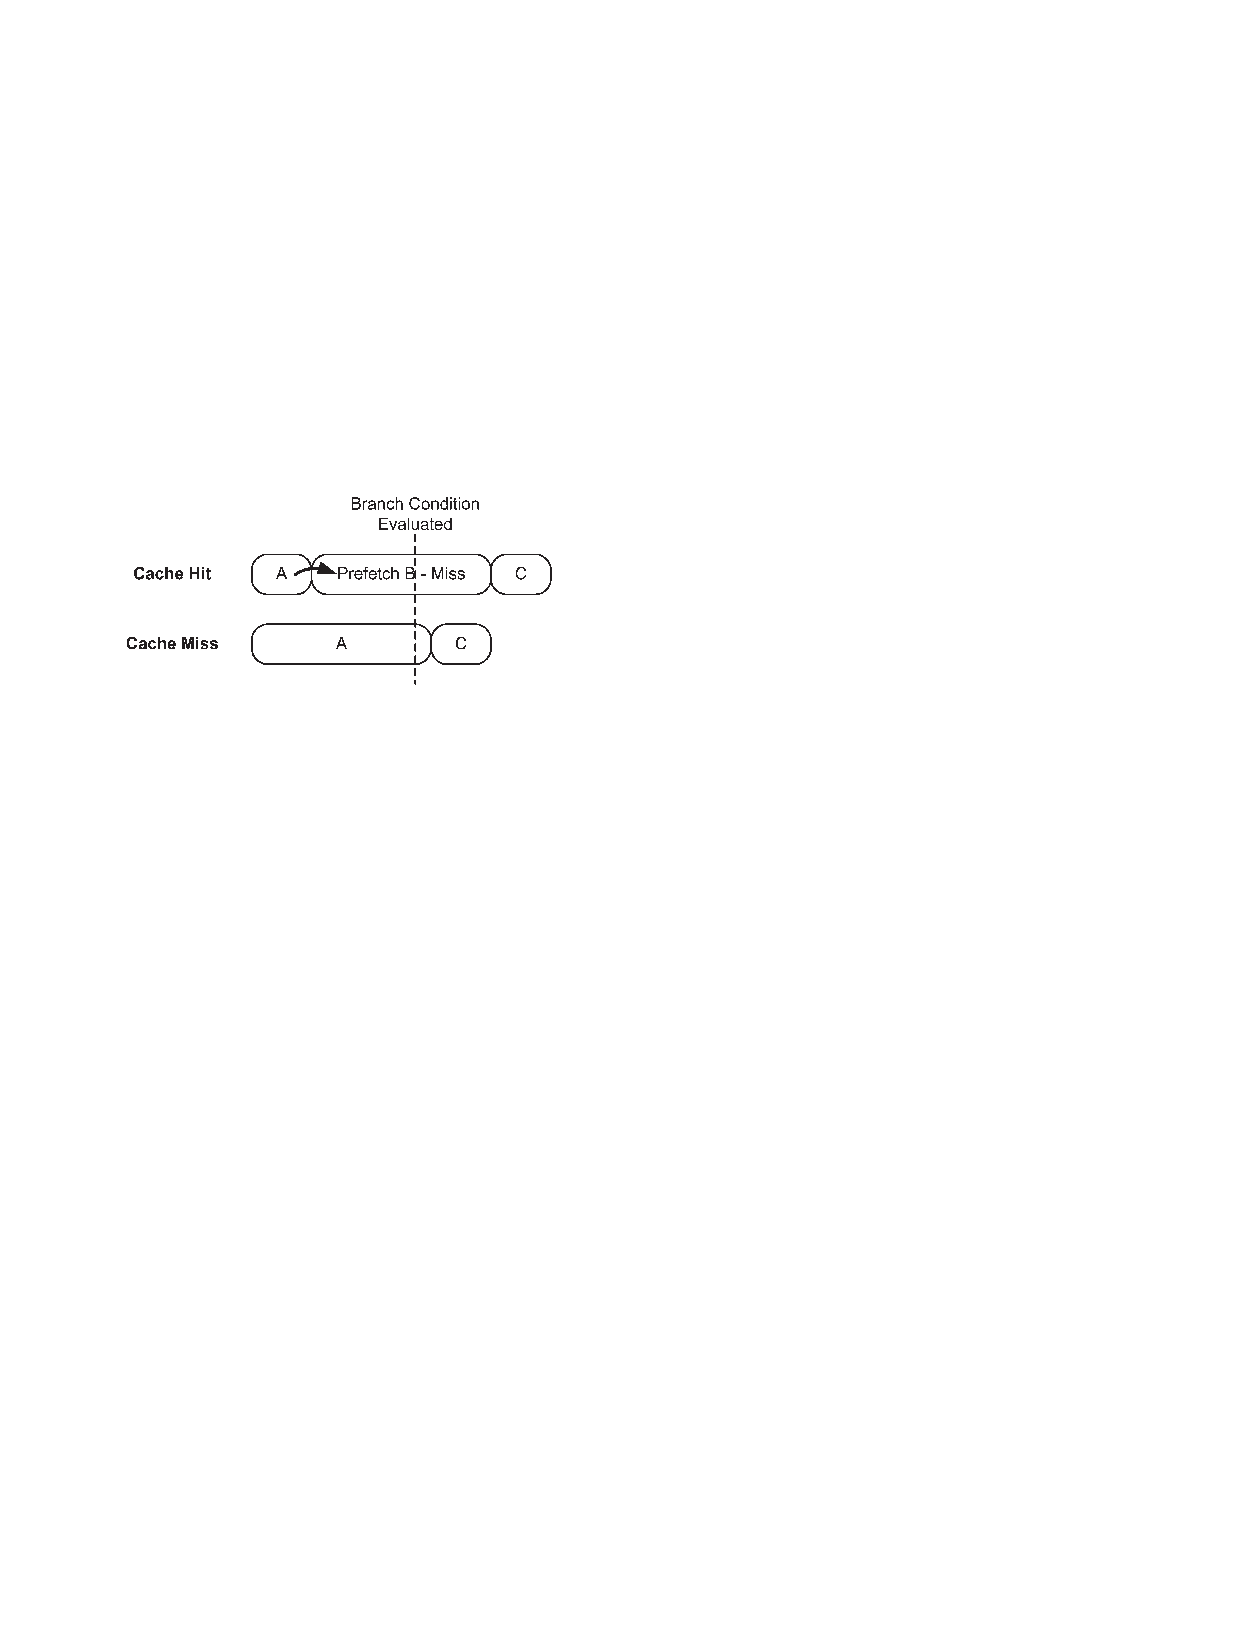
\includegraphics{figs/speculation_anomaly}
  \end{center}
  \vspace{-10pt}
  \caption{Timing anomaly cause by speculation~\cite{Reineke06adefinition}}
  \label{fig:speculation_anomaly}
  \vspace{-10pt}
\end{wrapfigure}
The common misconception is that at least a \emph{safe} upper bound on the execution time can be easily determined by assuming the worse case in unknown situations.
This is not true because dynamic processors can exhibit \emph{timing anomalies}~\cite{Reineke06adefinition,Lundqvist1999}; situations where a local worst-case does not result in the global worst-case.
Reineke et al.~\cite{Reineke06adefinition} illustrate this with the example shown in figure~\ref{fig:speculation_anomaly}.
In this example, a mispredicted branch results in unnecessary instruction fetching that destroys the cache state. 
However, if the first instruction being fetched is a cache miss, the correct branch condition will be computed before the fetch, and no speculatively executed instruction will destroy the cache state. 
This example shows that simply assume a cache miss (local worst-case) will not always lead to the global worst-case execution time.    

The increasing complexity of architectures leads to the conclusion that the usefulness of the results of WCET analysis strongly depends on the architecture of the employed processor~\cite{Heckmann2003processor}.
Modern processors employ features that improve average performance at the expense of worst-case performance, creating a large variation in execution time from the processor. 
These features are controlled and manage completely in hardware, not explicitly exposed to the software.
As a result, decrypting the state of the processor to obtain reasonable execution time estimates is often extremely difficult, if not impossible, on modern architectures.   

\section{Precision Timed Machines}
% As Wilhelm et al. \cite{Wilhelm_future_arch_09} quoted:
% \begin{quote} \textit{
%   ``The applicability of the AUTOSAR idea depends on availability of
%   architectures on which software composition does not lead to
%   unpredictable timing behavior.''
% }
% \end{quote}
In this thesis we present the design and implementation of a Precision Timed (PRET) machine~\cite{edwards2007case} -- the Precision Timed ARM (PTARM).
PTARM employs a thread-interleaved pipeline and a memory controller designed for predictable and composable execution.
It also implements an extended ARM~\cite{armrefman} ISA to demonstrate the ISA extensions with temporal semantics.
Our benchmarks show that an architecture designed for timing predictability and composability does not need to sacrifice performance.
%, and provides a robust, non brittle foundation for future cyber-physical systems.       

Many people have contributed to the results given in this thesis. 
The predictable DRAM controller that is presented in section~\ref{sec:pret_dram_controller} is a collaborative effort jointly done with Jan Reineke and Sungjun Kim. 
Hiren Patel, Ben Lickly, Jan Reineke, David Broman and Edward Lee have all greatly contributed to timing extensions to the ISA presented in section~\ref{sec:programming_models}.
And finally, the engine fuel rail simulation application presented in section~\ref{sec:1dCFD} is a collaborated effort with Matthew Viele, Guoqiang Wang and Hugo Andrade.
It is a pleasure to thank those who made this thesis possible, as this thesis could not have been complete without them. 
 
% In the remaining chapters we first discuss the design decisions of the hardware and ISA extensions in chapter~\ref{chapter:pret}, then show the details and architecture of PTARM in chapter~\ref{chapter:ptarm}.
% In chapter~\ref{chapter:app} we present two applications implemented with the PRET machine to demonstrate its applicability.
% Finally, in chapter~\ref{chapter:related} we discuss the related research work, and conclude in chapter~\ref{chapter:summary}.

% The remaining chapters are organized as follows. 
% Chapter~\ref{chapter:pret} explains the architecture of PRET including the \thdint pipeline and memory hierarchy, Chapter~\ref{chapter:ptarm}, Chapter~\ref{chapter:app}, Chapter~\ref{chapter:related}, Chapter~\ref{chapter:summary}.

%We aim to present architectures
%proposed a paradigm shift in the design of computer architectures, focusing on timing predictability instead of average-case performance.
%provide better wcet
%use thread-interleaved pipline and dram controller
%ISA extensions
%needed for autosar etc




% \begin{itemize}
% \item \emph{Low jitter} -- Small variance in execution time for a given code block, enabling a tight WCET bound.
% \item \emph{Continuous}~\cite{Henzinger2008} -- small changes in the input result in small changes in the output.
% \item Precise timing control, which is the ability to control temporal
%   properties in the architecture.
% \item Reasonable performance, or else someone could use a processor
%   from 20 years ago to achieve some of the effects above.
% \item Repeatable performance, mainly that the same execution yields
%   the same output. Including execution time. (\textcolor{red}{This
%     needs careful defining... what counts as input and what counts as
%     output?})
% \item Composability - The ability to compose two tasks without
%   interference. This is an extremely important property to preserve
%   because when we design systems, we want to design larger systems
%   from smaller components. We want to test those smaller systems
%   separately, then compose them and still have those tested properties
%   hold true. 
% \end{itemize}
% Through this, enable evaluation on the effects and implications on the composition, communication and synchronization of software components or tasks on a predictable architecture.





\chapter{Precision Timed Machine}
\label{chapter:pret}
In this chapter we present the design principles of a PREcision Timed (PRET) Machine.
Specifically, we discuss the implementation of a predictable pipeline and memory controller, and present timing extensions to the ISA. 
It is important to understand why and how current architectures fall short of timing predictability and repeatability.
Thus, we first discuss the common architectural designs and their effects on execution time, and point out some key issues and trade-offs when designing architectures for predictable and repeatable timing.

\section{Pipelines}
The introduction of pipelining vastly improved the performance of processors.
Pipelining increases the number of instructions that can be processed at one time by splitting up instruction execution into multiple steps.
It allows for faster clock speeds, and improves instruction throughput compared to single cycle architectures.
Ideally each in processor cycle, one instruction completes and leaves the pipeline as another enters and begins execution. 
In reality, different pipeline hazards occur which reduce the throughput and create stalls in the pipeline.
The techniques introduced to mitigate the penalties of pipeline hazards greatly effect to the timing predictability and repeatability of architectures.     
We analyze several commonly used techniques to reduce the performance penalty from hazards, and show their effects on execution time and predictability. 

\subsection{Pipeline Hazards}
\label{sec:pipeline_hazards}
\subsubsection{Data Hazards}

\begin{wrapfigure}{r}{0.5\textwidth}
  \vspace{-30pt}
  \begin{center}
    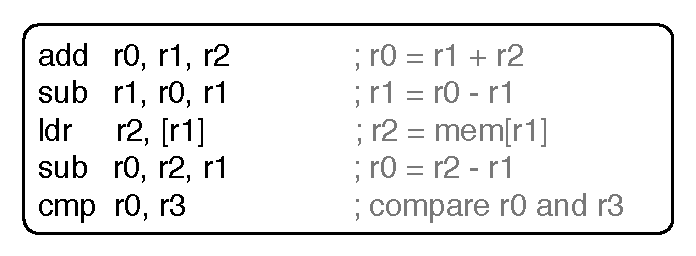
\includegraphics[scale=.65]{figs/sample_data_dependent_code}
  \end{center}
  \vspace{-3mm}
  \caption{Sample code with data dependencies}
  \label{fig:sample_data_dependent_code}
\end{wrapfigure}

Data hazards occur when the data needed by an instruction is not yet available.
Pipelines begin the execution of instructions before preceding ones are finished, so consecutive instructions that are data-dependent could simultaneously be executing in the pipeline.
For example, the code in figure~\ref{fig:sample_data_dependent_code} shows assembly instructions from the ARM instruction set architecture (ISA) that each depend on the result of its previous instruction.
Figure~\ref{fig:data_depend_execution_non_interleaved} shows two ways data hazards are commonly handled in pipelines. 

\begin{figure}
\vspace{-20pt} 
\begin{center}
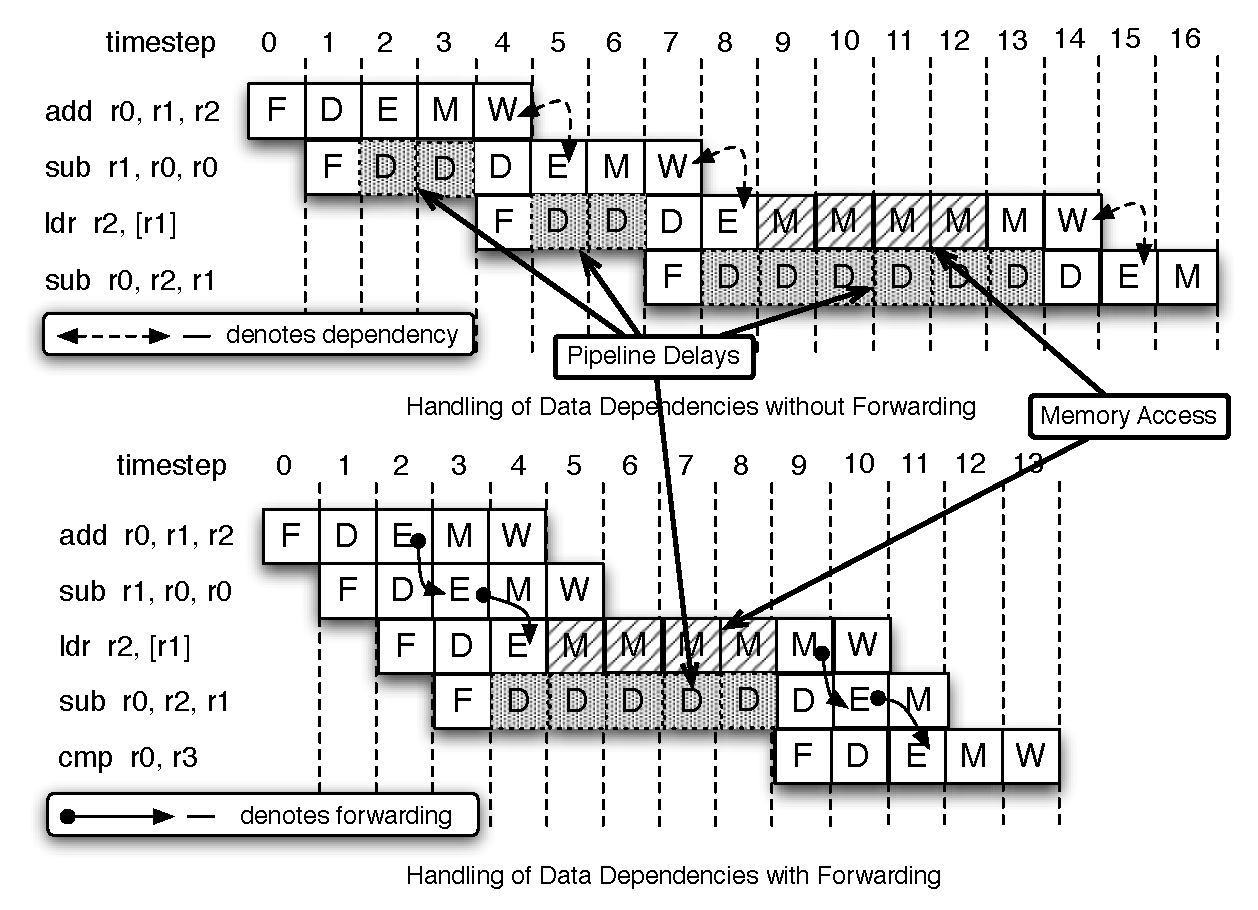
\includegraphics[scale=.6]{figs/data_depend_execution_non_interleaved}
\end{center}
\vspace{-3mm}
\caption{Handling of data dependencies in single threaded pipelines}
\label{fig:data_depend_execution_non_interleaved}
\end{figure}

In the figure, time progresses horizontally towards the right.
Each time step, or column, represents a processor cycle.
Each row represents an instruction that is fetched and executed within the pipeline.
Each block represents the instruction entering the different stages of the pipeline -- fetch (F), decode (D), execute (E), memory (M) and writeback (W).   
We assume a classic five stage RISC pipeline.

A simple but effective technique stalls the pipeline until the previous instruction completes.
This is shown in the top of figure~\ref{fig:data_depend_execution_non_interleaved}, as delays are inserted to wait for the results from previous instructions.
The dependencies between instructions are explicitly shown in the figure to make clear why the pipeline delays are necessary.
The performance penalty incurred in this case comes from the pipeline delays inserted.

\emph{Data forwarding} is commonly used to mitigate the need for inserting delays when data hazards occur.
Pipelines split up the execution of instructions into different execution stages. 
Thus, the results from an instruction could be ready, but waiting to be committed in the last stage of the pipeline.
Data forwarding utilizes this and introduces backwards data paths in the pipeline, so earlier pipeline stages can access the data from instructions in later stages that have not yet committed.
This greatly reduces the amount of delays inserted in the pipeline, as instructions can access the results of previous instructions before they commit.
The circuitry of data forwarding usually consists of the backwards data paths and multiplexers in the earlier pipeline stages to select the correct data to be used.    
The pipeline controller dynamically detects whether a data-dependency exists, and changes the selection bits of the multiplexers accordingly to select the correct operands.

The bottom of figure~\ref{fig:data_depend_execution_non_interleaved} shows the execution sequence of the previous example in a pipeline with data forwarding.
No pipeline delays are inserted for the first \emph{sub} and \emph{ldr} instruction because the data they depend on are forwarded with the forwarding paths.
However, delays are still inserted for the second \emph{sub} instruction after the \emph{ld} instruction.
For longer latency operations, such as memory accesses, the results are not yet available to be forwarded by the forwarding paths, so pipeline delays are still required. 
This illustrates the limitations of data forwarding.
They can address data hazards that result from pipelining, such as read-after-write register operations, but they cannot address data hazards that result from long latency operations, such as memory operations.
More involved techniques such as the out-of-order execution or superscalars are required to mitigate the effects of long latency operations.

The handling of data hazards in pipelines can cause instructions to exhibit dynamic execution times.  
For example, figure~\ref{fig:data_depend_execution_non_interleaved} shows the \emph{sub} instruction, in both top and bottom figures, exhibiting different execution times. 
To determine the execution time of instructions on pipelines that stall for data hazards, we need to determine when a stall is inserted, and how long the pipeline is stalled for.
Stalls are required when the current instruction uses the results of a previous instruction that is still in execution in the pipeline.
Thus, depending on the pipeline depth, a window of previous instructions needs to be checked to determine if any stalls are inserted.     
The length of the stall is determined by the execution time of the dependent instruction, because the pipeline will stall until that instruction completes.
Data forwarding does not remove the data hazards, but only reduces the number of stalls required to take care of the data hazards.  
Thus, to determine the execution time when data forwarding is used, timing analysis needs to determine when the data forwarding circuitry cannot not forward the data for data hazards.
This can similarly be done by observing the window of instructions not yet committed in the pipeline.  
The difference is, instead of all data dependencies, only data dependencies from long latency operations need to be detected.

Both techniques used for handling data hazards caused the execution time of instructions to depend on a window of previous instructions.
The deeper the pipeline, the larger the window of instructions execution time will depend on. 
Thus, static execution time analysis needs to model and account for this additional the window of instructions on pipelined architectures that use stalling or forwarding to handle the data hazards. 

\subsubsection{Control Hazards}
\begin{wrapfigure}{r}{0.5\textwidth}
  \vspace{-20pt}
  \begin{center}
    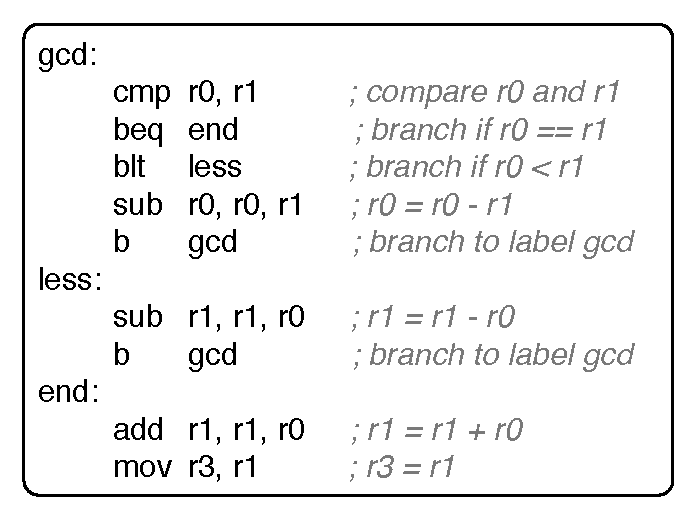
\includegraphics[scale=.65]{figs/sample_gcd_code}
  \end{center}
  \vspace{-3mm}
  \caption{GCD with conditional branches}
  \label{fig:sample_gcd_code}
\end{wrapfigure}

Branches are the most common cause of control-flow hazards (or control hazards) in the pipeline; the instruction after the branch, which should be fetched the next cycle, is unknown until after the branch instruction is completed.
Conditional branches further complicates matters, as whether or not the branch is taken depends on an additional condition that could also be unknown when the conditional branch is in execution. 
The code segment in figure~\ref{fig:sample_gcd_code} implements the \emph{Greatest Common Divisor} (GCD) algorithm using the conditional branch instructions \emph{beq} (branch equal) and \emph{blt} (branch less than) in the ARM ISA.  
Conditional branch instructions in ARM branch based on conditional bits that are stored in a processor state register.
Those conditional bits can be set based on the results of standard arithmetic instructions \todo{cite arm manual}.
The \emph{cmp} instruction is one such instruction that subtracts two registers and sets the conditional bits according to the results.
The GCD implementation shown in the code uses this mechanism to determine whether to continue or end the algorithm.
Figure~\ref{fig:branch_execution_non_interleaved_pipeline} shows the execution of the conditional branches from our example, and demonstrates two commonly used techniques to handling control hazards in pipelines. 
To show only the timing effects of handling control hazards, we assume an architecture with data forwarding that handles data hazards.
As there are no long latency instructions in our example, all stalls observed in the figure are caused by the handling of control hazards.  

\begin{figure}
\begin{center}
\noindent\makebox[\textwidth]{%
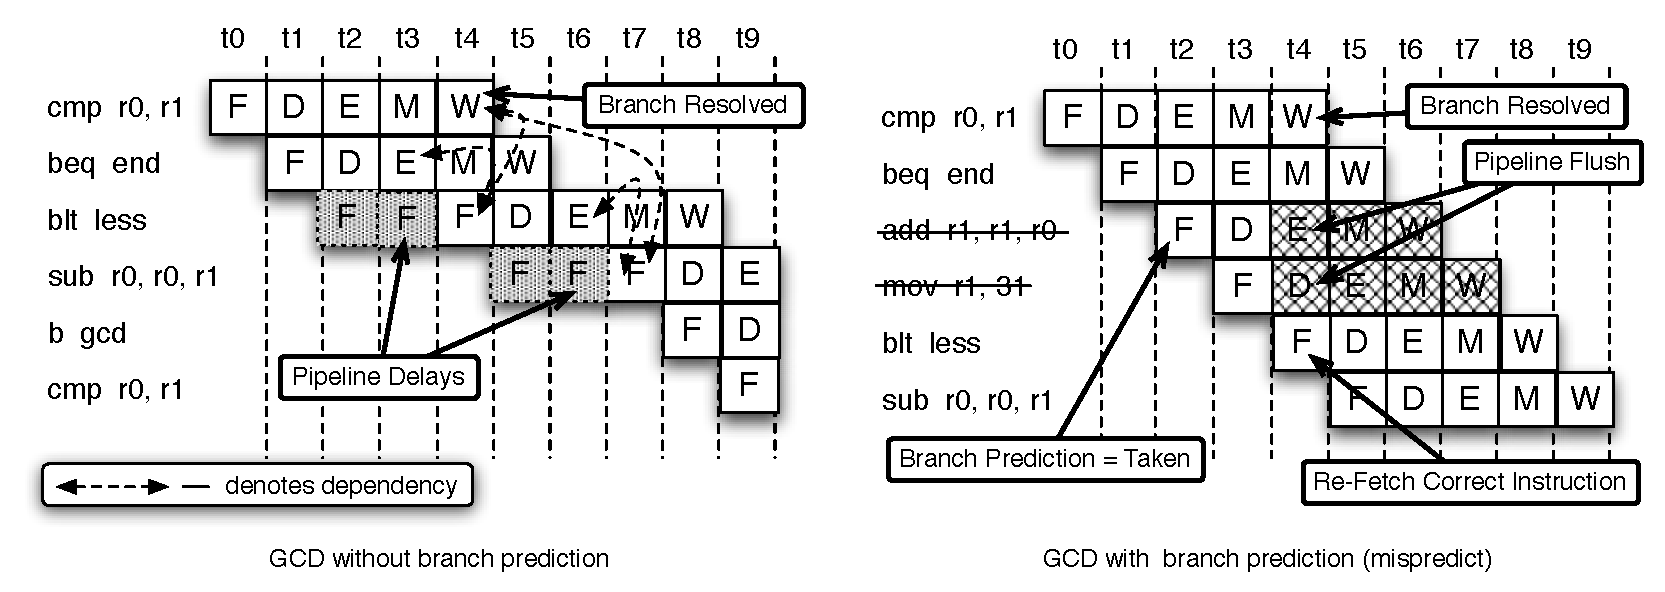
\includegraphics[scale=.58]{figs/branch_execution_non_interleaved_pipeline}}
\end{center}
\vspace{-3mm}
\caption{Handling of conditional branches in single threaded pipelines}
\label{fig:branch_execution_non_interleaved_pipeline}
\end{figure}

Similar to data hazards, control hazards can also be handled by stalling the pipeline until the branch instruction completes. 
This is shown on the left of figure~\ref{fig:branch_execution_non_interleaved_pipeline}. 
%The dependencies between instructions are explicitly shown to make clear why the pipeline delays are necessary.
Branch instructions typically calculate the target address in the execute stage, so two pipeline delays are inserted before the fetching of the \emph{blt} instruction, to wait for \emph{beq} to complete the target address calculation. 
The reasoning applies to the two pipeline delays inserted before the \emph{sub} instruction. 
The performance penalty (often referred to as the \emph{branch penalty}) incurred in this case is the two delays inserted after every branch instruction, to wait for the branch address calculation to complete.

To mitigate the branch penalty, some architectures enforce the compiler to insert one or more non-dependent instructions after each branch instruction.
These instruction slots are called branch delay slots, and are always executed before the pipeline branches to the target address. 
This way, instead of wasting cycles to wait for the target address calculation, the pipeline continues to execute useful instructions before it branches.
However, if the compiler cannot place useful instructions in the branch delay slot, \emph{nops} need to be inserted into those slots to ensure correct program execution.
Thus, branch delay slots are less effective for deeper pipelines because more delay slots need to be filled by the compiler to account for the branch penalty.
  
Instead of stalling, \emph{branch predictors} are commonly employed to predict the branch condition and target address so the pipeline can speculatively continue execution. 
Branch predictors internally maintain some form of state machine that is used to determine the prediction of each branch.  
The internal state is updated after each branch according to the results of the branch. 
Different prediction schemes have been proposed, and some can even accurately predict branches up to 93.5\%\todo{citation}.  
If the branch prediction is correct, no penalty is incurred for the branch because the correct instructions were speculatively executed.  
%With branch predictor, the pipeline fetches the next instruction based upon the results of the branch prediction, and continues to execute speculatively.
However, when the prediction is incorrect (often referred as a \emph{branch midpredict}), the speculatively executed instructions are flushed, and the correct instructions are re-fetched into the pipeline for execution.

The right of figure~\ref{fig:branch_execution_non_interleaved_pipeline} shows the execution of GCD in the case of a branch misprediction.
The \emph{beq} branch is predicted to be taken, so the \emph{add} and \emph{mov} instructions from label \emph{end} are directly fetched into execution. 
When \emph{beq} progresses past the execute stage, \emph{cmp} has forwarded its results used to determine the branch condition, and the branch target address has been calculated, so the branch is resolved.
At this point, the misprediction is detected, so the \emph{add} and \emph{mov} instruction are flushed out of the pipeline. 
The next instruction from the correct path, the \emph{blt} instruction, is immediately re-fetched, and execution continues.
The performance penalty of branch mispredictions is derived from the number of pipeline stages between instruction fetch and branch resolution.  
In our example, the misprediction penalty is 2, as branches are resolved after the execute stage.
This penalty only occurs on a branch mispredict, thus branch predictors with high success rates typically improve average performance of pipelines drastically, compared to architectures that simply stall for branches.
%However, for more complex architectures with caches or other hardware states, the effects of incorrectly fetched instructions on the state of the processor less well-known and studied. 

The two methods of handling control hazards exhibit vastly different effects on execution time.    
When stalls are used to handle control hazards, the execution time effects are static and predictable.   
The pipeline will simply \emph{always} insert pipeline delays after a branch instruction.
Thus, no extra complexity is added to the execution time analysis; the latency of branch instructions simply need to be adjusted to include the branch penalty.
On the other hand, if a branch predictor is employed, the execution time of each branch will vary depending on the result of the branch prediction.  
To determine the success of a branch prediction, both the prediction and the branch outcome, both of which can dynamically change in run-time, must be known.   
Program path analysis can attempt to analyze the actual outcome of branches statically from the program code. 
The predictions made from the branch predictor depend on the internal state stored in the hardware unit.
This internal state, updated by each branch instruction, must be explicitly modeled in order to estimate the prediction. 
If the predictor state is unknown, the miss penalty must conservatively be accounted for.
There has been work on explicitly modeling branch predictors for execution time analysis\todo{citation}, but the results are \todo{the results of branch predictor modeling for execution time analysis}.
To make matters worse, the speculative execution on the predicted program paths lead to further complications that need to be accounted for.
Other internal states exist in the architecture that could be affected by speculatively executing instructions.
For example, if caches were used, their internal state could be updated during speculative execution of a mispredicted path.
As architectures grow in complexity, the combined modeling of all hardware states in the architecture often lead to an infeasible explosion in state space for the analysis.    
This makes a tight static execution time analysis extremely difficult, if not impossible.

The difference in execution time effects between stalling and employing a branch predictor highlight an important trade-off for architecture designs.    
It is possible to improve average-case performance by making predictions, and speculatively executing based upon them.
However, this comes at the cost of predictability, and a potential prolonging of the worst-case performance.  
For real-time and safety critical systems, the challenge remains to improve worst-case performance while maintaining predictability.
How pipeline hazards are handled play an integral part of tackling this challenge.           
 
Although less often mentioned, the presence of interrupts and exceptions in the pipeline also create control hazards. 
Exceptions can occur during the execution of any instruction, and changes the control flow of the program to execute the exception handler.
For single threaded pipelines, this means that all instructions fetched and not committed in the pipeline are speculative, because when an exception occurs, all uncommitted instructions in the pipeline become invalid.
Pipelines often handle this by flushing all instructions and fetching the exception handler for execution.      
These effects are acknowledged, but often ignored in static analysis because it is simply impossible to model every possible exception, and its effect on the architecture states. 
 
\subsubsection{Structural Hazards}
\emph{Structural hazards} occur when a processor's hardware component is needed by two or more instructions at the same time. 
For example, a single memory unit accessed both in the fetch and memory stage results in a structural hazard. 
The design of the pipeline plays an integral part in eliminating structural hazards. 
For example, the classic RISC five stage pipeline only issues one instruction at a time, and uses separate instruction and data caches to avoid structural hazards.
Structural hazards are generally much more prevalent in architectures that issue multiple instructions at a time.
If structural hazards cannot be avoided, then the pipeline must stall to access the contended hardware component sequentially.
The execution time effects of structural hazards are specific to how contention is managed for each pipeline design.
Here we omit a general discussion of the timing effects, and later address them specifically for our proposed architecture. 

\subsection{Pipeline Multithreading}
Discussed above, \emph{data forwarding} and \emph{branch prediction} are simple techniques employed to handle pipeline hazards. 
Advanced architectures, such as \emph{superscalar} and \emph{VLIW} machines, employ more complex mechanisms to improve the average performance of the architecture.  
Both architectures issue multiple instructions every cycle, and superscalar machines dynamically execute instructions out-of-order if no dependency is detected.    
These architectures exploit \emph{instruction-level parallelism} to overlap the execution of instructions from a single thread whenever possible.         
On the contrary, \emph{multithreaded architectures} exploit \emph{thread-level parallelism} to overlap the execution of instructions from different hardware threads. 
Each hardware thread in a multithreaded architecture has its own physical copy of a processor state, such as the registers file and program counter etc.
When a pipeline hazard arises from the execution of a hardware thread, another hardware thread can be fetched for execution to avoid stalling the pipeline. 
This improves the instruction throughput of the architecture.

\begin{figure}[h]
\begin{center}
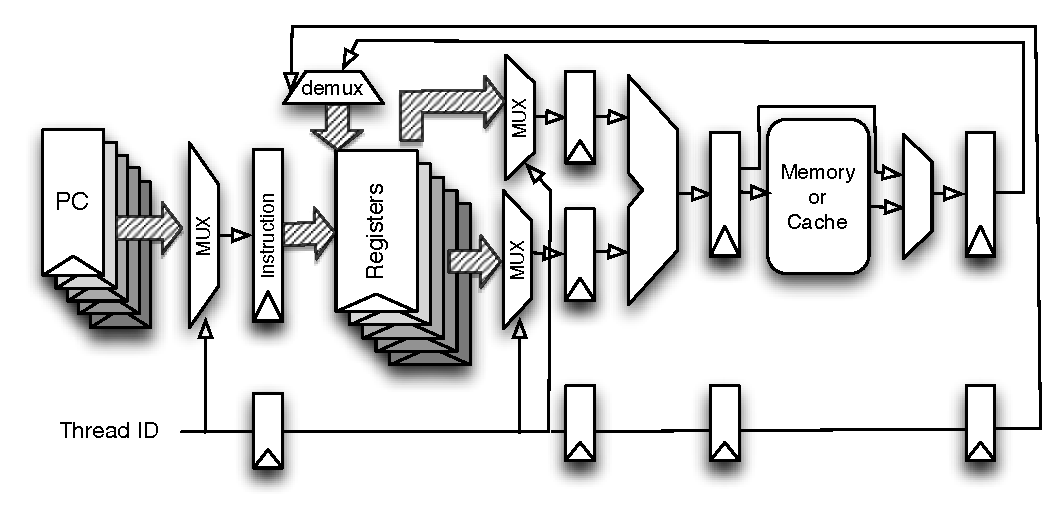
\includegraphics[scale=.8]{figs/multithreaded_pipeline_block}
\end{center}
\vspace{-10pt}
\caption{Simple Multithreaded Pipeline}
\label{fig:multi-thread pipeline simplified}
\end{figure}
Figure~\ref{fig:multi-thread pipeline simplified} shows the implementation of a simple multithreaded pipeline.
It contains 5 hardware threads, so it has 5 copies of the Program Counter (PC) and Register files.
The rest of the pipeline remains similar to a classic five stage RISC pipeline, with the addition of a few multiplexers used to select the thread states.
Thus, the extra copies of the processor state and multiplexers are most of the hardware additions needed to implement hardware multithreading.
When a hardware thread executes in the pipeline, its corresponding thread state is passed into the pipeline to be used.
In most of this thesis, the term \emph{threads} to refer to the explicit hardware threads that have hardware copies of the thread state.
This is not to be confused with the common notion of \emph{threads}, which describes software contexts managed by an operating system, with its states stored in memory.
It will be explicitly noted when we refer to the software notion of threads. 
%The selection of threads for execution is one of the most important factors to fully utilize thread-level parallelism.
%If a thread is stalled waiting for memory access but gets selected to execute in the pipeline, then that instruction slot is wasted and the processor isn't fully utilized.
Ungerer et al.~\cite{Ungerer:2003:survey_multithreading} surveyed different multithreaded architectures and categorized them based upon the \emph{thread scheduling} policy and the \emph{execution width} of the pipeline.

The \emph{thread scheduling} policy determines which threads are executing, and how often a context switch occurs.  
\emph{Coarse-grain} policies manage threads similar to the way operation systems manage software threads.
A thread gains access to the pipeline and continues to execute until a context switch is triggered.
Context switches occur less frequently via this policy, so less threads are required to fully utilize the processor.
Different coarse-grain policies trigger context switches with different events. 
Some policies trigger context switches on dynamic events, such as a cache miss or an interrupt; some policies trigger context switches on more static events, such as specialized instructions.
\emph{Fine-grain} policies switch context much more frequently -- some as frequent as every processor cycle.
The \emph{execution width} of the pipeline is to the number of instructions fetched each cycle.  
Multithreaded architectures with wider pipeline widths can fetch all instructions a single thread, or mix instructions from different threads.
The Sumultanous Multithreaded (SMT) architecture~\todo{cite} is an example where instructions are fetched from different threads each cycle.

Multithreaded architectures present several challenges for static execution time analysis.
As figure~\ref{fig:multi-thread pipeline simplified} illustrated, threads share the hardware components within the pipeline.
If a hardware component, such as a branch predictor, maintains internal state, that internal state can be modified by all threads in the pipeline.
As the internal states of the hardware components affect the execution time of the individual instructions, each thread can affect the execution time of all threads in the pipeline. 
If the threads' execution time are interdependent, their timing cannot be separately analyzed.
As a result, in order to precisely model the hardware states, the execution order of instructions from all threads need to be known.
The interleaving of threads depend heavily on the thread scheduling policy, execution width, and hazard handling logic employed in the pipeline.
The compounding effect of these can create an overwhelming combination of possible thread interleavings, making static timing analysis nearly impossible, even if only a conservative estimation is desired.   

Nonetheless, we contend that thread-level parallelism (TLP) \emph{can} be exploited to handle pipeline hazards predictably. 
Even the most sophisticated architectures that fully exploit instruction-level parallelism (ILP) cannot guarantee enough parallelism in a single instruction stream to remove all stalls caused by pipeline hazards. 
This is known as the \emph{ILP Wall}~\todo{cite}. 
Conventional multithreaded architectures use coarse-grain thread scheduling policies to dynamically exploit TLP when there is not enough ILP to be exploited.    
However, the compounding effects of the combined architectural features lead to unpredictable architectural timing behaviors.
Instead, a \emph{thread-interleaved pipeline} fully exploits TLP with a fine-grained thread scheduling policy.
We show that with several predictable architectural adjustments to the thread-interleaved pipeline, we can achieve a fully time-predictable pipeline 
with deterministic execution time behaviors.     

\subsection{A Predictable Thread-Interleaved Pipeline}
\label{section:pret_thread_pipeline}
Thread-interleaved pipelines use a fine-grain thread scheduling policy; every cycle a different hardware thread is fetched for execution.
A round robin scheduling policy is often employed to reduce the context switch overhead every cycle.     
The thread-interleaved pipeline is known for implementing the peripheral processors of the Cray Multi-Threaded Architecture (MTA) multiprocessors~\todo{cite}.
Each the ``peripheral processor'' is implemented as a hardware thread.     
Interacting with input/output peripherals often lead to idle processor cycles that waits for the peripherals' responses.
By interleaving several threads, thread-level parallelism is fully exploited, and the idle cycles can be used for simultaneous interaction with multiple input/output devices.       
Figure~\ref{fig:execution_thread_interleaved_pipeline} shows an example execution sequence from a 5 stage single width thread-interleaved pipeline with 5 threads.
\begin{figure}[h]
    \begin{center}
    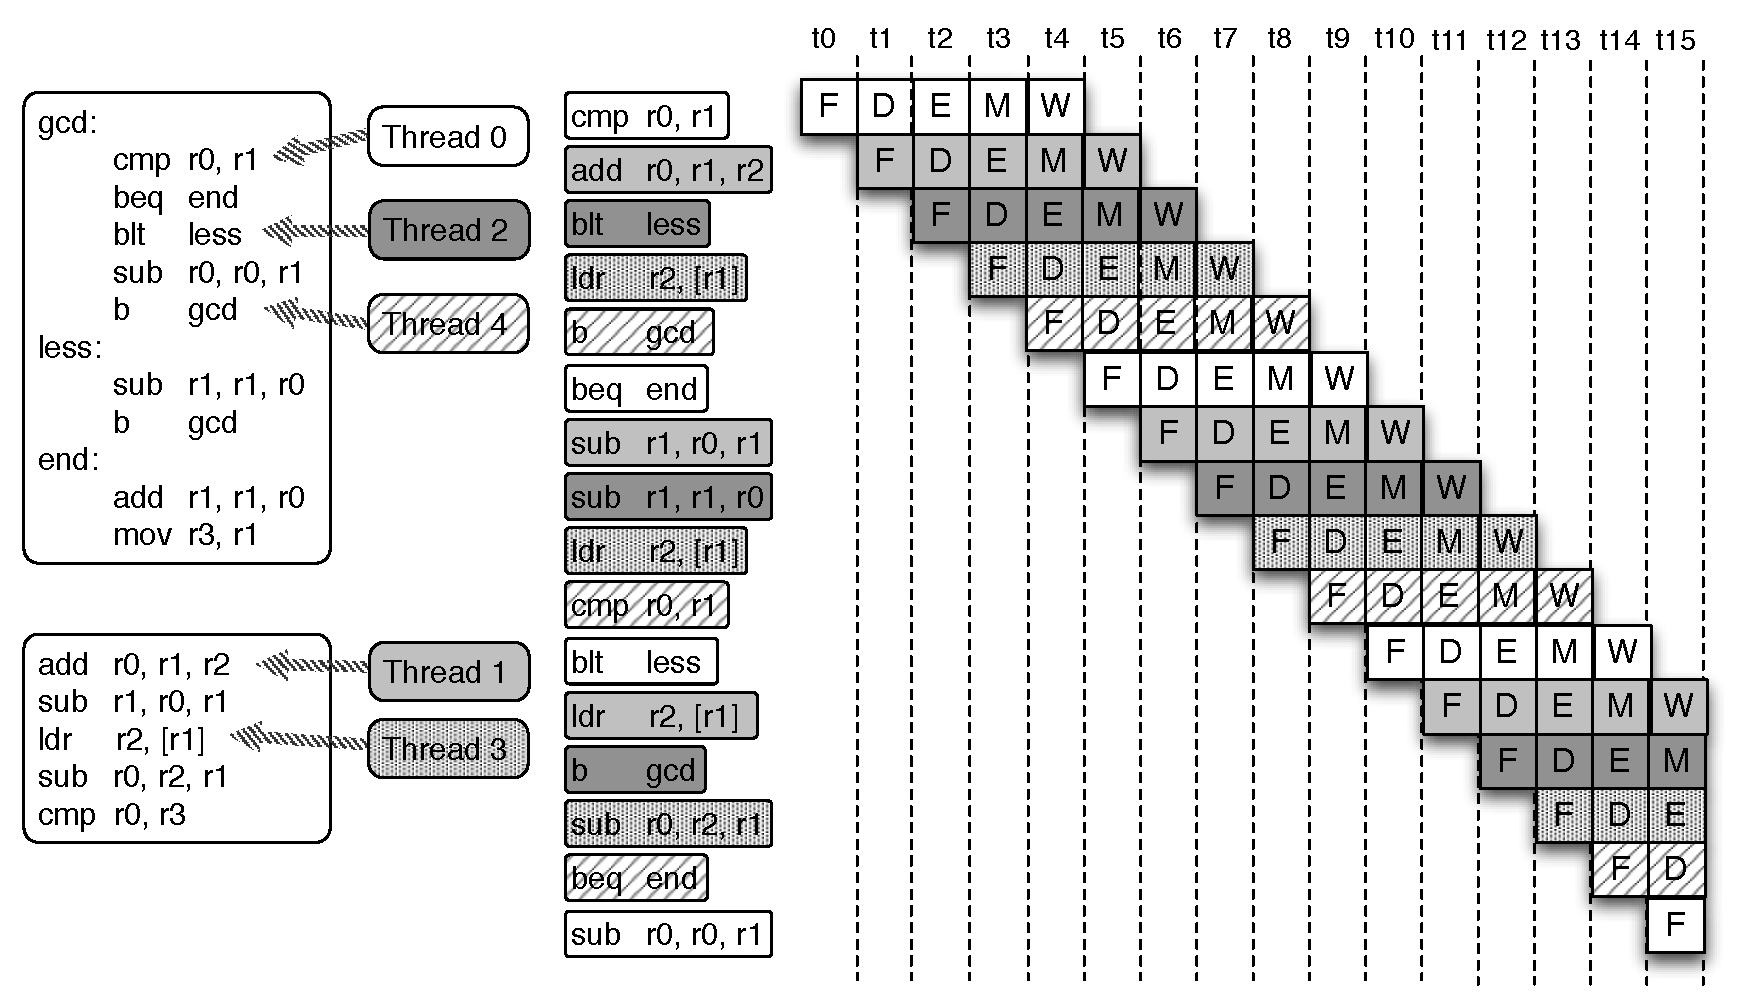
\includegraphics[scale=.55]{figs/thread-interleaved-execution}
  \end{center}
  \vspace{-10pt}
  \caption{Sample execution sequence of a thread-interleaved pipeline with 5 threads and 5 pipeline stages}
  \label{fig:execution_thread_interleaved_pipeline}
\end{figure}

The same code segments from figure~\ref{fig:sample_gcd_code} and figure~\ref{fig:sample_data_dependent_code} are used in this example. 
Threads 0, 2 and 4 execute GCD (figure~\ref{fig:sample_gcd_code}) and threads 1 and 3 execute the data dependent code segment (figure~\ref{fig:sample_data_dependent_code}).
The thick arrows on the left show the initial execution progresses of each thread at time 0.
We observe from the figure that each time step, an instruction from a different hardware thread is fetched in round robin order.
By time step 4, each pipeline stage is occupied by a different hardware thread.
The fine-grained thread interleaving and round robin scheduling combine to form this important property for thread-interleaved pipelines, which provides the basis for a timing predictable pipeline design.

The interleaving of threads by itself does not guarantee timing predictability for the pipeline.  
Shared hardware components or a selective thread execution policy can easily allow the execution time of threads to be affected by each other.    
As previously discussed, a combined timing analysis of all threads in the pipeline is extremely difficult, if not impossible.
In order for multithreaded architectures to achieve predictable performance, threads must be temporally isolated from one another. 
Temporal isolation removes cross-thread timing dependencies to allows timing analysis of threads independently.
This enables a simple and more precise execution time analysis.  
We refine several features on the thread-interleaved pipeline to temporally isolate the threads and predictably handle pipeline hazards.
This establishes a time-predictable thread-interleaved pipeline.

\subsubsection{Control Hazards}
By interleaving enough threads, control hazards can be completely removed from the pipeline.
This effect can be observed and explained from the execution sequence shown in figure~\ref{fig:execution_thread_interleaved_pipeline}.
At time 2, a \emph{blt} instruction from thread 2 is fetched into the pipeline.
On a single-threaded pipeline, stalls or branch prediction would be required to fetch the instruction at the next time step.
In this example, the next instruction fetched belongs to thread 3, and does not depend on the branch results of the \emph{blt} instruction.
No control hazard occurs from the branch, so no stall or branch prediction is needed to fetch the instruction.
The instruction fetch that depends on the branch result occurs at time 7.
Again, there is no control hazard since the branch is resolved by this point, so the instruction from the correct program path is fetched.    
Because control hazards from branches are eliminated, branch predictors are not needed in our pipeline design. 
Removing the branch predictor contributes to the temporal isolation of threads, as the shared internal state of the  branch predictor can create execution time dependencies between threads.  

The interleaving of threads also eliminate control hazards in the presence of exceptions.
If the pipeline detects an exception for the \emph{blt} instruction in the writeback stage (time 6), the control flow for thread 2 is changed to handle the exception.  
Because no other instruction in the pipeline belongs to thread 2 at time 6, no instruction needs to be flushed.  
This reveals an important property our timing predictable pipeline, that \emph{no instruction is speculatively executed}.
The next instruction fetch from thread 2 does not occur until time 7.
At that point, any control flow change, including one caused by an exception, is already known.
Therefore, the correct program path is always executed.

The minimum number of threads required to eliminate control hazards depend on the number of the pipeline stages.
Conservatively, employing the same number of threads as pipeline stages will always remove control hazards.
Intuitively, this is because at any point in time, each stage of the pipeline with be executing an instruction from a different hardware thread. 
Thus, no explicit dependency exists between instructions in the pipeline. 
However, Lee and Messerschmitt~\cite{lee1987pip} show that it is possible to use one less thread than the number of pipeline stages.
From here on, when we refer to the thread-interleaved pipeline, we assume enough threads to remove explicit dependencies between instructions in the pipeline.

\subsubsection{Data Hazards}
Because no explicit dependencies exist between instructions in the pipeline, data hazards that stem from the pipeline of instructions are removed. 
However, long latency operations can still cause data hazards in a thread-interleaved pipeline. 
This happens when a long latency operation is not completed before the next instruction fetch from the thread.
Although thread-interleaved pipelines can continue to fill the pipeline with other threads, data hazards are not completely eliminated.   
If all threads simultaneously execute a long latency operation, then no thread will be available to fill the pipeline. 

To maximizes pipeline utilization and instruction throughput, thread-interleaved pipelines can mark threads inactive when a long latency operation occurs.   
However, this dynamic behavior leads to non-trivial timing effects for the pipeline 
First, as stated earlier, a minimum number of threads is required to remove control hazards and the explicit dependencies between instructions in the pipeline. 
By allowing threads to be inactive, it is possible for the number of active threads to fall below this minimum. 
This can be circumvented by inserting pipeline stalls when the number active threads falls below the minimum.
This is illustrated in figure~\ref{fig:three_thread_pipeline}.
\begin{figure}[h]
  \vspace{-10pt}
  \begin{center}
    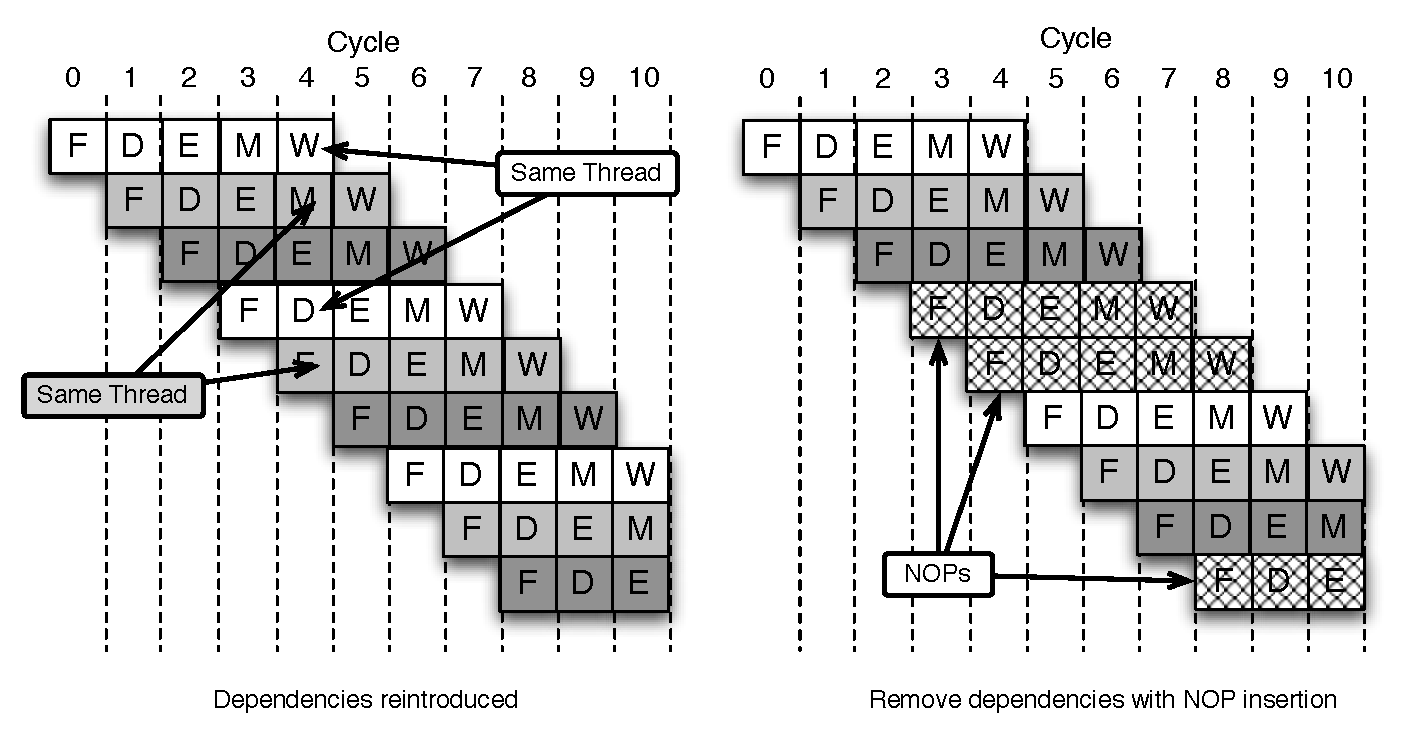
\includegraphics[scale=.6]{figs/three_thread_pipeline}
  \end{center}
  \vspace{-10pt}
  \caption{Execution of 5 threads thread-interleaved pipeline when 2 threads are inactive}
  \label{fig:three_thread_pipeline}
\end{figure}
This example shows the interleaving of 3 out of 5 threads in a 5 stage pipeline. 
We assume that 2 threads are inactive waiting for memory accesses.    
On the left we see that explicit dependency for instructions in the pipeline are reintroduced.
Only by inserting pipeline stalls to meet the minimum required thread count (shown on the right), can we assure that these dependencies are removed.   
The amount of stalling can be reduced if more threads are interleaved in the pipeline, since there is a larger pool of threads to select from. 
However, it is not possible to guarantee that stalls are never needed. 

More importantly, the dynamic activation and deactivation of threads breaks temporal isolation between the threads.   
When a thread is deactivated, other threads are fetched more frequently into the pipeline.
Thus, the execution frequency of threads would depend on number of active threads.
In order to maintain temporal isolation between the threads, our timing predictable thread-interleaved pipeline does not deactivate threads dynamically when long latency operations occur.

Instead, the thread scheduling policy of 

Although this slightly reduces the utilization of the thread-interleaved pipeline, but threads are decoupled and timing analysis can be done individually for each thread without interference from other threads.
At the same time, we still preserve most of the benefits of latency hiding, as other threads are still executing during the long latency operation.

%The next instruction from thread 3 that is fetched into the pipeline is again the same \emph{ld} instruction.  
%As memory completes its execution during the execution of instructions from other threads, we replay the same instruction to pick up the results from memory and write it into registers to complete the execution of the \emph{ld} instruction. 
%It is possible to directly write the results back into the register file when the memory operation completes, without cycling the same instruction to pick up the results.
%This would require hardware additions to support and manage multiple write-back paths in the pipeline, and a multi write ported register file, so contention can be avoided with the existing executing threads.
%In our design we simply replay the instruction for write-backs to simplify design and piggy back on the existing write-back datapath.

Because no explicit dependencies exist between instructions in the pipeline, data hazards that stem from the pipeline of instructions are removed. 
Thus, the forwarding logic normally used to handle data hazards are not needed in thread interleaved pipelines. 
Data forwarding logic contain no internal state, so threads can remain temporally isolated even if they are present.   
However, the pipeline design is greatly simplified in the absence of forwarding logic and branch predictors.   
This enables thread-interleaved pipelines to be clocked at faster clock speeds, because less logic exists between the pipeline stages.
  
\subsubsection{Structural Hazards}
Shared hardware units within multithreaded architectures could also easily break temporal isolation amongst the threads. 
Two main issues arise when a hardware unit is shared between the threads. 
The first issue arises when shared hardware units share the same state between all threads. 
If the state of hardware unit is shared and can be modified by any thread, then it is nearly impossible to get a consistent view of the hardware state from a single thread during timing analysis.
Shared branch predictors and caches are prime examples of how a shared hardware state can cause timing inference between threads.
If a multithreaded architecture shares a branch predictor for all threads, then the branch table entries can be overwritten by branches from any thread.
This means that each thread's branches can cause a branch mispredict for any other thread. 
Caches are especially troublesome when shared between threads in a multithreaded architecture. 
Not only does it make the execution time analysis substantially more difficult, it also decreases overall performance for each thread due to cache thrashing, an event where threads continuously evict each other threads cache lines in the cache\todo{citation}.
To achieve temporal isolation between the threads, the hardware units in the architecture must not share state between the threads. 
Each thread must have its own consistent view of the hardware unit states, without the interference from other threads.
For example, each thread in our thread-interleaved pipeline contains its own private copy of the registers and thread states.    
We already showed why thread-interleaved pipelines do not need branch predictors because they remove control-hazards, and we will discuss a timing predictable memory hierarchy that uses scratchpads instead of caches in section~\ref{section:memory_system}.
The sharing of hardware state between threads also increases security risks in multithreaded architectures. 
Side-channel attacks on encryption algorithms\todo{cite} take advantage of the shared hardware states to disrupt and probe the execution time of threads running the encryption algorithm to crack the encryption key.
We will discuss this in detail in section~\ref{sec:app_side_channel_attack} and show how a predictable architecture can prevent timing side-channel attacks for encryption algorithms.   

The second issue that arises is that shared hardware units create structural hazards -- hazards that occur when a hardware unit needs to be used by two or more instructions at the same time.
Structural hazards typically occur in thread-interleaved pipelines when the shared units take longer than one cycle to access. 
The ALU, for example, is shared between the threads.
But because it takes only one cycle to access, there is no contention even when instructions continuously access the ALU in subsequent cycles.
On the other hand, a floating point hardware unit typically takes several cycles to complete its computation.
If two or more threads issue a floating point instruction in subsequent cycles, then contention arises, and the the second request must be queued up until the first request completes its floating point computation.   
This creates timing interference between the threads, because the execution time of a floating point instruction from a particular thread now depends on if other threads are also issuing floating point instructions simultaneously. 
If the hardware unit can be pipelined to accept inputs every processor cycle, then we can remove the the contention caused by the hardware unit, since accesses no longer need to be queued up.
The shared memory system in a thread-interleaved pipeline also creates structural-hazards in the pipeline.
In section~\ref{section:memory_system} we will discuss and present our memory hierarchy along with a redesigned DRAM memory controller that supports pipelined memory accesses.
%The assumption here is still that we have a single issue pipeline architecture.   
If pipelining cannot be achieved, then any timing analysis of that instruction must include a conservative estimation that accounts for thread access interference and contention management.
Several trade-offs need to be considered when deciding how to manage the thread contention to the hardware unit.

A time division multiplex access (TDMA) schedule to the hardware unit can be enforced to decouple the access time of threads remove timing interference.
A TDMA access scheme certainly creates an non-substantial overhead compared to conventional queuing schemes, especially if access to the hardware unit is rare and sparse.
However, in a TDMA scheme, each threads wait time to access the shared resource depends on the time offset in regards to the TDMA schedule, and is decoupled from the accesses of other threads.
Because of that, it is possible obtain a tighter worst case execution time analysis per thread.
For a TDMA scheme, the worst case access time occurs when an access just missed its time slot and must wait a full cycle before accessing the hardware unit.
For a conventional queuing scheme where each requester can only have one outstanding request, the worst case happens when every other requester has a request in queue, and the first request is just beginning to be serviced.   
At first, it may seem that the worst case execution time of a TDMA scheme may seem similar to the basic queuing scheme.
For timing analysis at an unknown state of the program, no assumption can be made on the TDMA schedule, thus the worst case time must be used for conservative estimations. 
However, because the TDMA access schedule is static, and access time is decoupled from other threads, there is potential to obtain tighter timing analysis for accesses by inferring access slot hits and misses for future accesses. 
For example, based upon the execution time offsets of a sequence of accesses to the shared resource, we may be able to conclude that at least one access will hit its TDMA access slot and get access right away.
We can also possibly derive more accurate wait times for the accesses that do not hit its access slots based upon the elapsed time between accesses.
An in depth study of WCET analysis of TDMA access schedules is beyond the scope of the thesis.
But these are possibilities now because there is no timing interference between the threads. 
A queue based mechanism would not be able to achieve better execution time analysis without taking into account the execution context of all other threads in the pipeline.

\bigskip

\todo{Compare execution sequences of previous figures of threads. Highlight the simpler timing analysis}

\todo{highlight that the observable latency of long latency instructions are predictably reduced}
For operations that have long latencies, such as memory operations or floating point operations, thread-interleaved pipelines hides the latency with its execution of other threads. 
Thread 3 in figure~\ref{fig:execution_thread_interleaved_pipeline} shows the execution of a \emph{ld} instruction that takes the same 5 cycles as shown in figure~\ref{fig:data_depend_execution_non_interleaved}.
We again assume that this \emph{ld} instruction accesses data from the main memory. 
While the \emph{ld} instruction is waiting for memory access to complete, the thread-interleaved pipeline executes instructions from other threads.

It is important to understand that we are not proclaiming that all dynamic behavior in systems are harmful. 
But only by achieving predictability in the hardware architecture can we begin to reason about more dynamic behavior in software.
For example, we discussed that dynamically scheduling threads in hardware causes timing interference. 
However, it is not the switching of threads that is unpredictable, but how the thread switching is triggered that makes it predictable.   
For example, the Giotto\todo{cite} programming model specifies a periodic software execution model that can contain multiple program states. 
If such a programming model was implemented on a thread-interleaved pipeline, different program states might map different tasks to threads or have different number of threads executing within the pipeline.
But by explicitly controller the thread switches in software, the execution time variances introduced is transparent at the software level, allowing potential for timing analysis.

%TODO: Talk about the trade-offs of threaded interleaved pipelines to summarize 
In this section we introduced a predictable thread-interleaved pipeline design that provides temporal isolation for all threads in the architecture.
The thread-interleaved pipeline favors throughput over single thread latency, as multiple threads are executed on the pipeline in a round robin fashion.  
We will present in detail our implementation of this thread-interleaved pipeline in chapter~\ref{chapter:ptarm}, and show how the design decisions discussed in this chapter are applied.

\section{Memory System}
\label{section:memory_system}
While pipelines designs continue to improve, memory technology has been struggling to keep up with the increase in clock speed and performance.
Even though memory bandwidth can be improved with more bank parallelization, the memory latency remains the bottleneck to improved memory performance.
Common memory technologies used in embedded systems contain a significant tradeoff between access latency and capacity. 
Static Random-Access Memories (SRAM) provide a shorter latency that allows single cycle memory access from the pipeline.
However, the hardware cost to implement each memory cell prevents SRAM blocks from being implemented with high capacity.
On the other hand, Dynamic Random-Access Memories (DRAM) use a more compact memory cell design that can easily be combined into larger capacity memory blocks.
But the memory cell of DRAMs must be constantly refreshed due to charge leakage, and the large capacity memory blocks often prohibit faster access latencies.
%TODO: talk about about embedded systems seldom need disk?
To bridge the latency gap between the pipeline and memory, smaller memories are placed in between the pipeline and larger memories to act as a buffer, forming a memory hierarchy.
The smaller memories give faster access latencies at the cost of lower capacity, while larger memories make up for that with larger capacity but slower access latencies. 
The goal is to speed up program performance by placing commonly accessed values closer to the pipeline and placing less accessed values farther away.

\subsection{Memory Hierarchy}
\subsubsection{Caches}
\begin{wrapfigure}{r}{0.5\textwidth}
  \vspace{-20pt}
  \begin{center}
    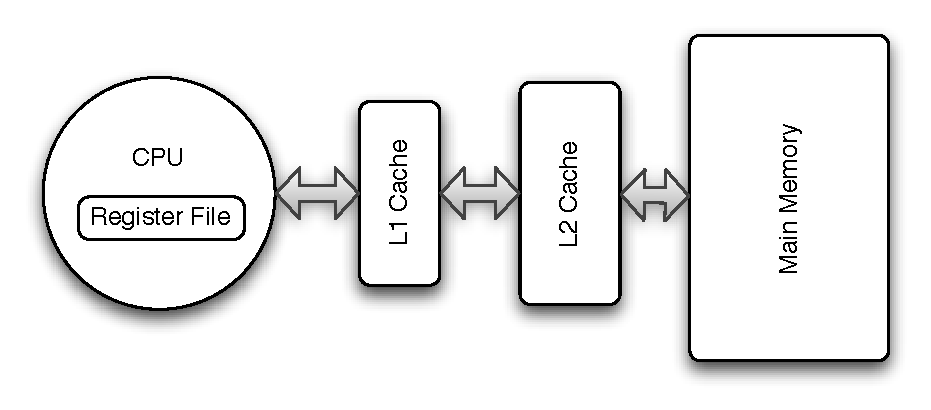
\includegraphics[scale=.5]{figs/conventional_mem_hierarchy}
  \end{center}
  \vspace{-20pt}
  \caption{Memory Hierarchy w/ Caches}
  \label{fig:conventional_mem_hierarchy}
  \vspace{-10pt}
\end{wrapfigure}   
A \emph{CPU Cache} (or cache) is commonly used in the memory hierarchy to manage the smaller fast access memory made of SRAMs.
The cache manages the contents of the fast access memory in hardware by leveraging the spatial and temporal locality of data accesses. 
The main benefits of the cache is that it abstracts away the memory hierarchy from the programmer.
When a cache is used, all memory accesses are routed through the cache. 
If the data from the memory access is in the cache, then a cache hit occurs, and the data is returned right away.
However, if data is not in the cache, then a cache miss occurs, and the cache controller fetches the data from the larger memory and adjusts the memory contents in the cache. 
The replacement policy of the cache is used to determine which cache line, the unit of memory replacement on caches, to replace. 
A variety of cache replacement policies have been researched and used to optimize for different memory access patterns of applications. 
In fact, modern memory hierarchies often contain multiple layers of hierarchy to balance the tradeoff between speed and capacity.
A commonly used memory hierarchy is shown in figure~\ref{fig:conventional_mem_hierarchy}.
If the data value is not found in the L1 cache, then it is searched for in the L2 cache. 
If the L2 cache also misses, then the data is retrieved from main memory, and sent back to the CPU while the L1 and L2 cache update its contents.
Different replacement policies can be used at different levels of the memory hierarchy to optimize the hit rate or miss latency of the memory access.

When caches are used, the program is oblivious to the different levels of memory hierarchy because they are abstracted away from the program; the cache gives its best-effort to optimize memory access latencies.
Whether or not an access hits the cache or goes all the way out to main memory is hidden from the program.
Thus, the programmer does not need to put in any effort, and can get a reasonable amount of performance. 
Furthermore, when programs are ported to another architecture with a different cache configuration, no change in the program is required to still obtain a reasonable amount of performance from the hardware.   
For general purpose applications, this gives the ability to improve design time and decrease design effort, which explains the cache's popularity. 

However, the cache makes no guarantees on actual memory access latencies and program performance. 
The execution time of programs could highly vary depending on a number different factors -- cold starts, previous execution contexts, interrupt routines, and even branch mispredictions that cause unnecessary cache line replacements.  
Thus, when execution time is important, the variability and uncontrollability of caches may outweigh the benefits they provide. 

The cache's internal states include the controller state and memory contents. 
As the programmer cannot explicitly control the state of the cache, it is extremely difficult to analyze execution time on systems with caches.
At an arbitrary point of execution, if the state of the cache is unknown, a conservative worst-case execution time analysis needs to assume the worst case, as if the memory access went directly to main memory.
In order to acquire tighter execution time analysis, the cache must be modeled with program execution to predict the cache state.
The ease of such modeling depends on the replacement policy used in the cache.

For example, the \emph{Least Recent Used} (LRU) replacement policy replaces the least recently used cache line whenever an eviction occurs. 
Within a basic block, a code segment without a control flow change, the contents of a cache with $N$ cache lines can be fully known after $N$ different memory accesses~\cite{Heckmann2003processor}.  
The $N$ different memory accesses will evict all cache lines in the cache prior to the basic block, and fill them with the memory contents of the $N$ accesses. 
In this case, the analysis assumes $N$ initial cache misses before the cache state is known.
However, the cache state is destroyed when analysis hits a control flow merge with another path.
Thus, the usefulness of this analysis depends on $N$ and how long basic blocks are in programs.  
In practice, the complexity of modern programs and memory architectures often introduce a high variability in program execution time, rendering analysis imprecise. 

Even outside of the context of real-time applications, caches can present unintended side effects.
For applications that require extreme high speed, the best-effort memory management that caches offer simply is not good enough.
Programs often need to be tuned and tailored to specific cache architectures and parameters to achieve the desired performance. 
In order to tune algorithm performance, algorithm designers are required to understand the abstracted away memory architecture and enforce data access patterns that conform to the cache size and replacement policy.   
For example, instead of operating on entire rows or columns of an array, algorithms are rewritten to operate on a subset of the data at a time, or blocks, so the faster memory in the hierarchy can be reused.
This technique is called \emph{Blocking}~\cite{Lam91thecache}, and is very well-known and commonly used.   
%\todo{talk about LAPACK? Libraries that tune programs to caching}.
%In this case, we see that the hidden memory hierarchy actually could degrade program performance.    

Multithreaded threaded architectures with shared caches among the hardware threads can suffer from \emph{cache thrashing}, an effect where different threads' memory accesses evict the cached lines of others.
With multiple hardware threads, it is extremely difficult for threads have any knowledge on the state of the cache, because it is simultaneously being modified by other threads in the system. 
As a result, the hardware threads have no control over which level in the memory hierarchy they are accessing, and the performance highly varies depending on what is running on other hardware threads. 

For multicore architectures, caches create a data coherency problem when data needs to be consistent between the multiple cores.
When the multiple cores are sharing memory, each core's private cache may cache the same memory address. 
If one core writes to a memory location that is cached in its private cache, then the other core's cache would contain stale data. 
Various methods such as bus snooping or implementing a directory protocol~\cite{Stenstrom:1990:SCC:79809.79810} have been proposed to keep the data consistent in all caches. 
Implementing a scalable and efficient cache coherence scheme is still a hot topic of research today.

\subsubsection{Scratchpads}
We cannot argue against the need for a memory hierarchy, as there is an undeniable gap between processor and DRAM latency.
However, instead of abstracting away the memory hierarchy, we propose to \emph{expose} the memory layout to the software.  

\emph{Scratchpads} were initially proposed for their power saving benefits over caches~\cite{Banakar2002}.
Scratchpads can be found in the Cell processor~\cite{cellproc}, which is used in Sony PlayStation 3 consoles, and NVIDIA's 8800 GPU, which provides 16KB of SPM per thread-bundle~\cite{8800gpu}.
Scratchpads use the same memory technology (SRAMs) as caches, but do not implement the hardware controller to manage their memory contents.
%Without the hardware controller, scratchpads do not manage its memory contents in hardware.
Instead, scratchpads occupy a distinct address space in memory when they are used as fast access memory.
Memory accesses that access the specific scratchpad address space will go to the scratchpad, and other accesses will go to main memory. 
Because in hardware scratchpads do not need to check whether the data is on the scratchpad or not, they have a reduced access latency, area and power consumption compared to caches~\cite{Banakar2002}. 

\begin{wrapfigure}{r}{0.45\textwidth}
  \vspace{-20pt}
  \begin{center}
    \includegraphics[scale=.5]{figs/pret_mem_hierarchy}
  \end{center}
  \vspace{-10pt}
  \caption{Memory Hierarchy w/ Scratchpads}
  \label{fig:pret_mem_hierarchy}
\end{wrapfigure}   

Unlike caches, which overlay their address space with main memory to hide the hierarchy, scratchpads explicitly \emph{expose} the memory hierarchy, as figure~\ref{fig:pret_mem_hierarchy} illustrates.  
The exposed memory hierarchy gives software full control over the management of memory contents in the hierarchy.
Data allocated on the scratchpad will have single cycle access latencies, while other data will take the full DRAM access latency. 
The memory access latency for each request now depends only on the access address, and not that state of another hardware controller. 
This drastically improves the predictability of memory access times, and removes the variability of execution time introduced with caches.
However, this places the burden of memory management on the programmer or compiler toolchains.  
The Cell processor~\cite{cellproc} is often criticized for being difficult to program, and one of the main reason is its use of scratchpads. 
Programmers have become accustomed to a uniform memory space, making it difficult to adjust to the non uniform memory space that must be explicitly managed.

Embedded system designs inherently need to deal with limited resources and other design constraints, such as limited memory or hard timing deadlines.    
Thus, the design of such systems often requires analysis of memory usage and latency to ensure that the constraints are met.
These analysis results can be used to generate automatic allocation schemes for scratchpads, lessening the burden on programmers.
Two allocation schemes are commonly employed to manage the contents of scratchpads in software.
\emph{Static allocation schemes} allocate data on the scratchpad during compile time, and the contents allocated on the scratchpad do not change throughout program execution. 
Static scratchpad allocation schemes~\cite{Suhendra2005WCETSPM, Patel2008PRETSPM} often use heuristics or a compiler-based static analysis of the program to find the most commonly executed instructions or data structures.
These are allocated statically on the scratchpad to improve program performance. 
\emph{Dynamic allocation schemes} modify the data on the scratchpad during run time in software through DMA mechanisms.
The allocation could either be automatically generated and inserted by the compiler, or explicitly specified by the user programmatically.
Higher level models of computation, such as Synchronous Dataflow (SDF)~\cite{lee_sdf} or Giotto~\cite{henzinger_giotto}, expose more structure and semantics of the model for better analysis, which can be used to optimize scratchpad allocation dynamically.
Bandyopadhyay~\cite{Bandyopadhyay06_AutomatedMemoryAllocationOfActorCodeDataBufferInHeterochronous} presents an automated memory allocation of scratchpads for the execution of Heterochronous Dataflow models.
The Heterochronous Dataflow (HDF) model is an extension to the Synchronous Dataflow (SDF) model with finite state machines (FCM). 
The HDF models contain different program states.
Each state executes a SDF model that contains actors communicating with each other. 
Bandyopadhyay analyzes the actor code and the data that is communicated in each HDF state, and derives an optimized scratchpad allocation for each state. 
The scratchpad allocation code is automatically inserted into the code to dynamically change the scratchpad contents during state transitions, so the memory allocation is optimized for the execution of each HDF state. 
This allocation not only shows roughly a 17\% performance improvement compared to executions using LRU caches, but also a more predictable program performance.

The underlying memory technology that is used to make both scratchpads and caches is not inherently unpredictable, as SRAMs provide constant low-latency access time. 
%However, caches manage the contents of the SRAM in hardware. 
However, by using caches in the memory hierarchy, the hierarchy is hidden from the programmer, and the hardware managed memory contents create highly variable execution times with unpredictable access latencies. 
Scratchpads on the other hand expose the memory hierarchy to the programmer, allowing for more predictable and repeatable memory access performances.
Although the allocation of scratchpads requires more programming effort, it also provides opportunity for high efficiency, as it can be tailored to specific applications.   
Thus, in our time-predictable architecture, scratchpads are employed as our fast-access memory. 

\subsection{DRAM Memory Controller}
Because of its high capacity, DRAMs are often employed in modern embedded systems to cope with the increasing code and data sizes.  
However, bank conflicts and refreshes within the DRAM can cause memory accesses to stall, further increasing the memory latency. 
Modern memory controllers are designed to optimize average-case performance by queueing and reordering memory requests to improve the throughput of memory requests. 
This results in unpredictable and varying access times along with an increased worst-case access time for each memory request.
In this section we will present a DRAM memory controller that privatizes DRAM banks with scheduled memory refreshes to provide improved worst-case latency and predictable access times.    
The contributions from this section are research done jointly with the several co-authors from Reineke et. al~\cite{ReinekeLiuPatelKimLee11_PRETDRAMControllerBankPrivatizationForPredictability}. 
We do not claim sole credit for this work, and the summary is included in this thesis only for completeness. 
We will first give some basic background on DRAM memories, then present the predictable DRAM controller designed.

\subsubsection{DRAM Basics}

\begin{figure}[h]
\begin{center}
\vspace{-8mm}
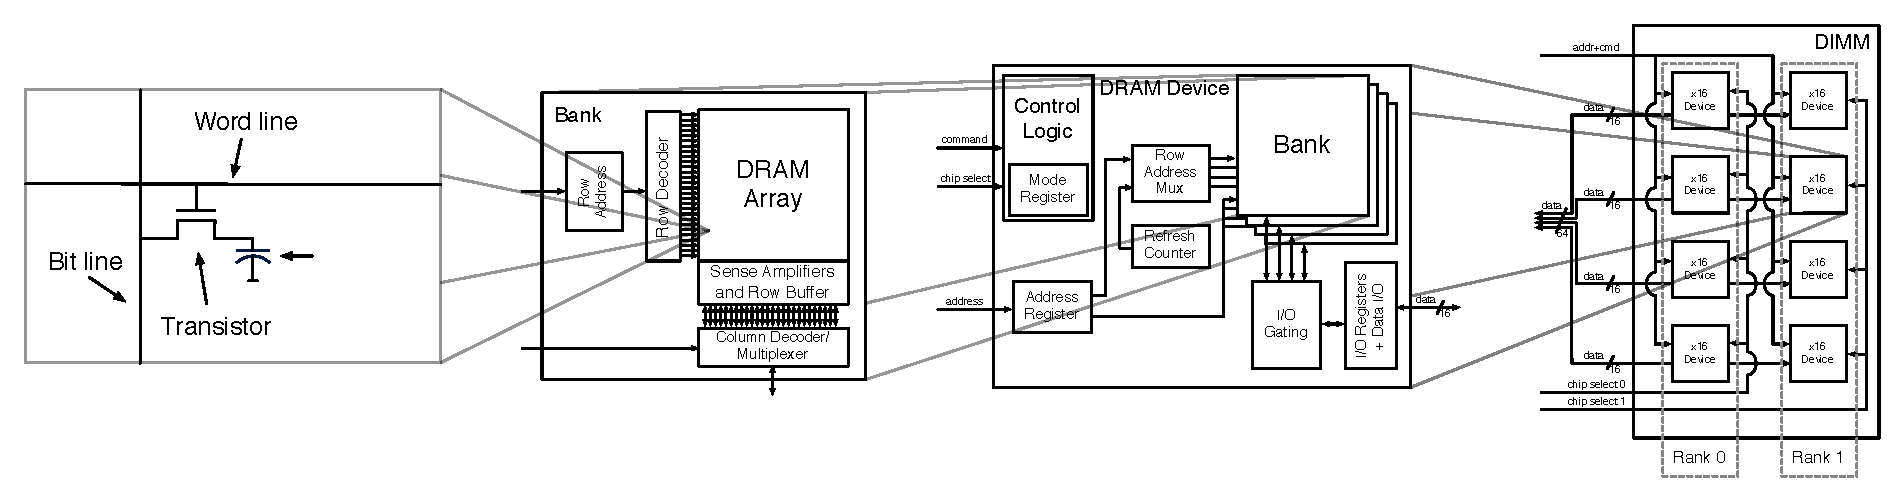
\includegraphics[width=\textwidth]{figs/dram-overview.pdf}
\vspace{-8mm}
\caption{A dual-ranked dual in-line memory module.}\label{fig:dram_basics}
\vspace{-5mm}
\end{center}
\end{figure} 

Figure~\ref{fig:dram_basics} shows the structure of a dual ranked in-line DDRII DRAM module.
Starting from the left, a basic \textbf{\emph{DRAM cell}} consists of a capacitor and a transistor. 
The capacitor charge determines the value of the bit, which can be accessed by triggering the transistor. 
Because the capacitor leaks charge, it must be refreshed periodically, typically every 64 ms or less~\cite{jedec}.

A \textbf{\emph{DRAM array}} is made of a two-dimensional array of DRAM cells.
Each access made to the DRAM array goes through two phases: a row access followed by one or more column accesses.   
During the row access, one of the rows in the DRAM array is moved into the row buffer.
To read the value in the row buffer, the capacitance of the DRAM cells is compared to the wires connecting them with the row buffer.
The wires need to be precharged close to the voltage threshold so the sense amplifiers can detect the bit value.
Columns can be read and written to quickly after the row is in the row buffer. 

The \textbf{\emph{DRAM device}} consists of banks formed of DRAM arrays. 
Modern DRAM devices have multiple banks, control logic, and I/O mechanisms to read from and write to the data bus, as shown in the center of figure \ref{fig:dram_basics}.
Banks can be accessed concurrently, but the data, command and address busses, which is what the memory controller uses to send commands to the DRAM device, are shared within the device. 
The following table\footnotemark\ lists the four most important commands and their function:
\footnotetext{This table is as shown in ~\cite{ReinekeLiuPatelKimLee11_PRETDRAMControllerBankPrivatizationForPredictability}}
%\begin{table}
\begin{center}
\begin{smalltabular}{p{13mm}p{6mm}p{10cm}}
Command 				& Abbr. & Description\\\hline
Precharge    			& PRE   & Stores back the contents of the row buffer into the DRAM array, and prepares the sense amplifiers for the next row access.\\
Row\hspace{13mm} access & RAS	& Moves a row from the DRAM array through the sense amplifiers into the row buffer.\\
Column access 			& CAS   & Overwrites a column in the row buffer or reads a column from the row buffer.\\
Refresh					& REF	& Refreshes several\footnotemark\ rows of the DRAM array. This uses the internal refresh counter to determine which rows to refresh.\\
\end{smalltabular}
%\caption{Overview of DDR2 Commands~\cite{ReinekeLiuPatelKimLee11_PRETDRAMControllerBankPrivatizationForPredictability}}
\label{tab:ddr2-commands}
\end{center}
%\end{table}
\footnotetext{The number of rows depends on the capacity of the device.}

To perform reads or writes, the controller first sends the PRE command to precharge the bank containing the data. 
Then, a RAS is issued to select the row, and one or more CAS commands can be used to access the columns within the row. 
Accessing columns from the same row does not require additional PRE and RAS commands, thus higher throughput can be achieved by performing column accesses in burst lengths of four to eight words.  
Column accesses can immediately be followed by a PRE command to decrease latency when accessing different rows. 
This is known as auto-precharge (or closed-page policy).
Refreshing of the cells can be done in two ways.
One common way is to issue a refresh command that refreshes all banks of the device simultaneously. 
The refresh latency depends on the capacity of the device, but the DRAM device manages a counter to step through all the rows.
The rows on the device could also be manually refreshed by performing row accesses to them.
Thus, the memory controller could perform row accesses on every row within the 64 ms refresh period.
This requires the memory controller to keep track of the refresh status of the device and issue more refresh commands, but each refresh takes less time because it is only a row access. 

\textbf{\emph{DRAM modules}} are made of several DRAM devices integrated together for higher bandwidth and capacity. 
A high-level view of the dual-ranked dual in-line memory module (DIMM) is shown in the right side of figure~\ref{fig:dram_basics}.
The DIMM has eight DRAM devices that are organized in two ranks.
The two ranks share the address, command inputs, and the 64-bit data bus.
The chip select is used to determine which ranks are addressed.
All devices within a rank are accessed simultaneously when the rank is addressed, and the results are combined to form the request response.  
% Due to the sharing of I/O mechanisms within a device, consecutive accesses to the same rank are more constrained than consecutive accesses to different ranks, which only share the command and address as well as the data bus.
% We later exploit this subtle difference by restricting consecutive accesses to different ranks to achieve more predictable access latencies.  
% We explain this in more detail in \ref{sec:pret_dram_controller}. 

Our controller makes use of a feature from the DDR2 standard known as posted-CAS.  
Unlike DDR or other previous versions of DRAMs, DDR2 can delay the execution of CAS commands (posted-CAS) for a user-defined latency, known as the additive latency ($AL$). 
Posted-CAS can be used to resolve command bus contention by sending the posted-CAS earlier than the corresponding CAS needs to be executed.

Table~\ref{table:ddr2-constraints} gives an overview of timing parameters for a DDR2-400 memory module.
These timing constraints come from the internal structure of DRAM modules and DRAM cells.
For example, $t_{RCD}, t_{RP}$, and $t_{RFC}$ are from the structure of DRAM banks that are accessed through sense amplifiers that need to be precharged.
$t_{CL}, t_{WR}, t_{WTR}$, and $t_{WL}$ result from the structure of DRAM banks and DRAM devices.
The four-bank activation window constraint $t_{FAW}$ constrains rapid activation of multiple banks that would result in too high of a current draw.
The memory controller must conform to these timing constraints when sending commands to the DDR2 module.  
%The additive latency, $t_{AL}$, can be set by the user and determines how many cycles after a posted-CAS a CAS is executed.
Here we only give a quick overview of DRAMs, we refer more interested readers to Jacob et al.~\cite{JaNgWa07} for more details.

\begin{table}[h]
\begin{center}
\begin{smalltabular}{l p{2.0cm} p{10cm}}
Parameter	& Value \footnotemark & Description \\\hline
$t_{RCD}$			& 3						& \textbf{Row-to-Column delay}: time from row activation to first read or write to a column within that row.\\
$t_{CL}$			& 3						& \textbf{Column latency}: time between a column access command and the start of data being returned.\\
$t_{WL}$			& $t_{CL}-1=2$			& \textbf{Write latency}: time after write command until first data is available on the bus.\\
$t_{WR}$			& 3						& \textbf{Write recovery time}: time between the end of a write data burst and the start of a precharge command.\\
%$t_{CCD}$			& $\burstlength/2$ 				& CAS to CAS command delay. Minimum time between two read commands or two write commands.\\
$t_{WTR}$ 			& 2 					& \textbf{Write to read time}: time between the end of a write data burst and the start of a column-read command.\\% Allows the sense amplifiers to restore the data in the DRAM array.\\
$t_{RP}$			& 3						& \textbf{Row precharge time:} time to precharge the DRAM array before next row activation.  \\
%$t_{RTRS}$			& 1\todo{check this}	& Rank-to-rank switching time.\\ 
$t_{RFC}$			& 21					& \textbf{Refresh cycle time}: time interval between a refresh command and a row activation.\\
%$t_{REFI}$			& 1560    				& Refresh to refresh interval \\
%$t_{RAS}$ 			& $t_{RCD}+t_{WL}+t_{WR} = 8$ & Minimum time after an activate command to a bank until that bank is allowed to be precharged.\\
%$t_{RC}$			& $t_{RAS}+t_{RP}=11$	& Row cycle time: minimum time between successive activate commands to the same bank.\\
%$t_{RTP}$			&   			& Minimum time between a precharge command on a bank and a successive activate command.\\
$t_{FAW}$			& 10					& \textbf{Four-bank activation window}: interval in which maximally four banks may be activated.\\
$t_{AL}$			& set by user			& \textbf{Additive latency}: determines how long posted column accesses are delayed.
\end{smalltabular}
%\todo{group constraints by their origin: constraints due to DRAM array structure, constraints due to sharing within DRAM device, constraints due to sharing of bus among ranks}
\end{center}
\caption{Overview of DDR2-400 timing parameters of the Qimonda HYS64T64020EM-2.5-B2.~\cite{ReinekeLiuPatelKimLee11_PRETDRAMControllerBankPrivatizationForPredictability}}\label{table:ddr2-constraints}
\end{table}
\footnotetext{In cycles at 200 MHz}

\subsubsection{Predictable DRAM Controller}
\label{sec:pret_dram_controller}
We will split the discussion of the predictable DRAM controller into its backend and frontend. 
The backend translates memory requests into DRAM commands that are sent to the DRAM module.
The frontend manages the interface to the pipeline along with the responsibility of scheduling refreshes.
Here we specifically refer to a DDR2 667MHz/PC2-5300 memory module operating at 200Mhz, which has a total size of 512MB over two ranks with four banks on each rank.
While our discussion of the design of this DRAM controller is specific to our DDR2 memory module, the key design features are applicable to other modern memory modules.

\paragraph{Backend}
Conventional DRAM memory controllers view the entire memory device as one resource, and any memory request can access the whole DRAM device. 
Subsequent memory accesses can target the same bank within the DRAM, which results in the need for memory requests to be queued and serviced sequentially, without exploiting bank parallelism.
Our controller views the memory devices as independent resources partitioned by banks. 
Specifically, we partition our memory module into four \emph{resources}, each consisting of two banks within the same rank. 
The banks within each resource can be arbitrarily chosen, but all banks within a resource must belong to the same rank, and each of the ranks must contain at least two resources.
This is to avert access patterns that would incur high latency from the contention for the shared busses within banks and ranks.
The partitioning of the memory device allows us to fully exploit bank parallelism by accessing the resources in a periodic and pipelined fashion.
The periodic access scheme to the four resources interleaves each memory access between the ranks.
Subsequent accesses to the same rank go to the other resource, grouped from banks.  
Figure~\ref{fig:backend} shows an example of the following access requests: read from resource 0 in rank 0, write to resource 1 in rank 1, and read from resource 2 in rank 0. 

\begin{figure}[h]
\begin{center}
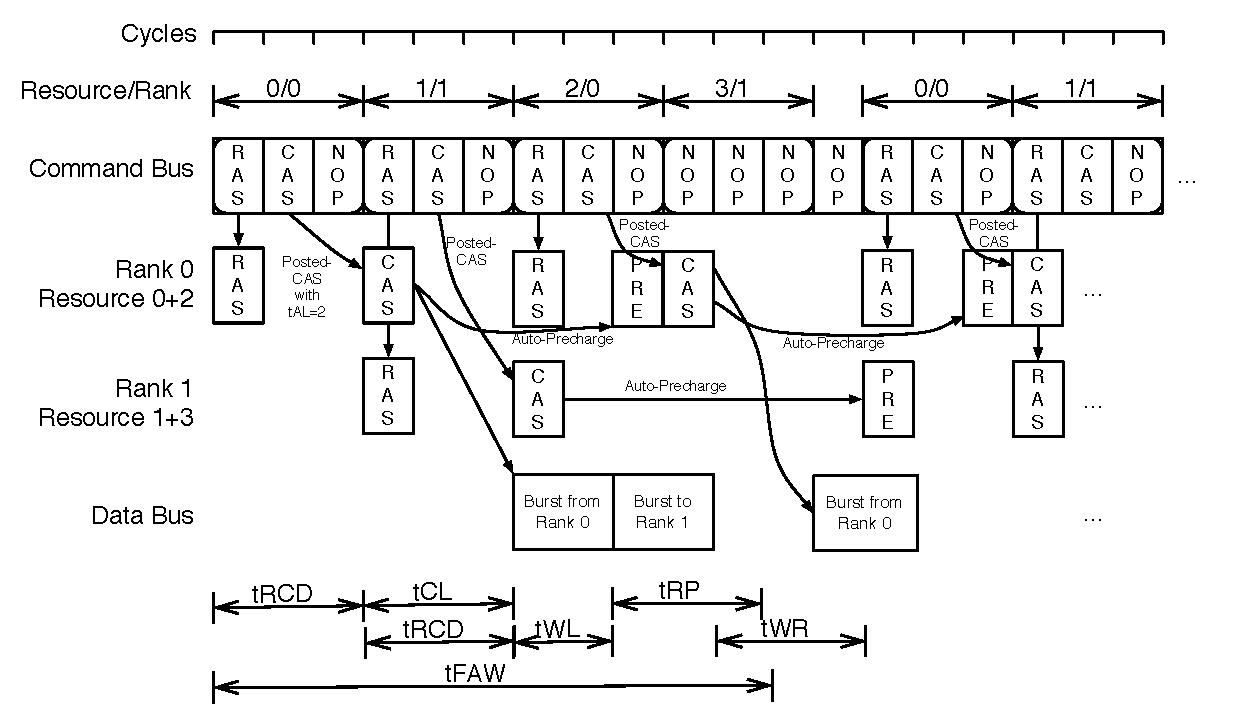
\includegraphics[width=0.92\linewidth]{figs/backend}
\end{center} 
\caption{The periodic and pipelined access scheme employed by the backend~\cite{ReinekeLiuPatelKimLee11_PRETDRAMControllerBankPrivatizationForPredictability}.}
\label{fig:backend}
\end{figure}

Each access request is translated into a RAS (Row Access), posted-CAS (Column Access) and NOP command. 
An access slot is formed of all three commands.  
The NOP command in the access slot is inserted between any two consecutive requests to avoid a collision on the data bus that occurs when a read request follows and a write request.
This collision is cause by the one cycle offset between the read and write latencies. 
The RAS command moves a row into the row buffer, and the CAS command accesses the columns within the row loaded into the row buffer. 
CAS commands can be either reads or writes, causing a burst transfer of $8 \cdot 4 = 32$ bytes that occupies the data bus for two cycles (as two transfers occur in every cycle).
We send a posted-CAS instead of a normal CAS in order to meet the row to column latency shown in table~\ref{table:ddr2-constraints}.
This latency specifies that the RAS command and the first CAS command need to be 3 cycles apart.  
However, manually issuing a CAS command to the first resource 3 cycles after its RAS command would cause a command bus conflict with the RAS command for the second resource.
Thus, we instead set the additive latency $t_{AL}$ to 2 and use the posted-CAS that offsets the CAS command to conform to the row to column latency.
This allows our memory controller to preserve our pipelined access scheme while meeting the latency requirements of the DRAM.   
We use a closed-page policy (also known as auto-precharge policy), which causes the accessed row to be immediately precharged after performing the column access (CAS), preparing it for the next row access.
If there are no requests for a resource, the backend does not send any commands to the memory module, as is the case for resource 3 in figure~\ref{fig:backend}.

Our memory design conforms to all the timing constraints listed in table~\ref{table:ddr2-constraints}.
The write-to-read timing constraint $t_{WTR}$, incurred by the sharing of I/O gating within ranks, is satisfied by alternating accesses between ranks. 
The four-bank activation window constraint is satisfied because within any window of size $t_{FAW}$ we activate at most four banks within the periodic access scheme. 
Write requests with the closed-page policy requires 13 cycles to access the row, perform a burst access, and precharge the bank to prepare for the next row access.
However, our periodic access scheme has a period of 12 cycles, as each access slot is 3 cycles, and there are four resources accessed. 
Thus, a NOP is inserted after the four access slots: to increase the distance between two access slots belonging to the same resource from 12 to 13 cycles.
As a result, the controller periodically provides access to the four resources every 13 cycles.
The backend does not issue any refresh commands to the memory module.
Instead, it relies on the frontend to refresh the DRAM cells using regular row accesses.

% \paragraph{Longer Bursts for Improved Bandwidth}
% Depending on the application, bandwidth might be more important than latency.
% Bandwidth can be improved by increasing the burst length from 4 to 8.
% Extending the proposed access scheme to a burst length of 8 is straightforward with the insertion of two additional NOP commands after each request to account for the extra two cycles of data being transfered on the data bus.  
% In this case, the access slot latency for each request is increased from three to five to include the extra two NOP commands, and data will be transferred in four out of five cycles rather than in two out of three.
% Then, of course, latency of transfers of size less than or equal to 32 bytes increases, but the latency of large transfers decreases and higher bandwidth is achieved. 

\begin{wrapfigure}{r}{0.5\textwidth}
\begin{center}
\vspace{-8mm}
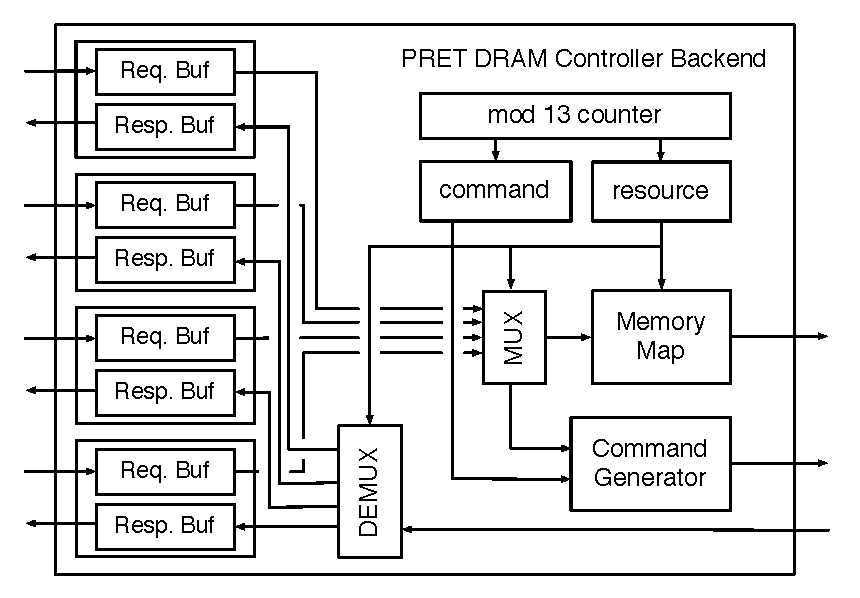
\includegraphics[width=1.1\linewidth]{figs/dram-backend-implementation}
\end{center}
\caption{Sketch of implementation of the backend~\cite{ReinekeLiuPatelKimLee11_PRETDRAMControllerBankPrivatizationForPredictability}.}
\label{fig:dram-backend-implementation}
\end{wrapfigure}

A high level block view of our backend implementation is shown in figure~\ref{fig:dram-backend-implementation}.
Each resource has a single request buffer and a respond buffer.
These buffers are used to interface with the frontend.   
A request is made of an access type (read or write), a logical address, and the data to be written for write requests. 
Requests are serviced at the granularity of bursts, i.e. 32 bytes in case of burst length 4 and 64 bytes in case of burst length 8.
A modulo-13 counter is used to implement the 13 cycle periodic access scheme in our controller.   
The ``resource'' and ``command" blocks are combinational circuits that are used to select the correct request buffer and generate the DRAM commands to be sent out. 
The ``memory map" block is where logical addresses are mapped to physical addresses that determine the rank, bank, row and column to access.
The data for read requests are latched into the response buffers to be read by the frontend.  

\paragraph{Frontend}
The frontend of our memory controller manages the interfacing to our backend, and the refreshing of the DRAM device.
The privatization of DRAM banks creates four independent resources that are accessed separately from the front end.
Thus, our memory controller is designed to be used by multicore or multithreaded architectures that contain multiple requesters which need access to the main memory.
Several recent projects, such as MERASA~\cite{Ungerer10}, PREDATOR~\cite{Akesson2007CODES}, JOP~\cite{Schoeberl2008265}, or CoMPSoC~\cite{Hansson09}, strive to develop predictable multi-core architectures that require predictable and composable memory performance.
These could potentially profit from using the proposed DRAM controller.

Specifically, we designed this memory controller to interface with the thread-interleaved pipeline discussed previously in section~\ref{section:pret_thread_pipeline}.
The thread-interleaved pipeline contains multiple hardware threads that each require access to main memory. 
We assign each hardware thread to a private memory resource, and send out memory requests to the memory controller frontend, which receives the request and places it within the request buffer.
Each thread in the thread-interleaved pipeline sends out only one outstanding memory request at a time, so the single request buffer for each resource is sufficient to interface with our thread-interleaved pipeline.
Once the request is serviced from the backend, the pipeline can read the data from the response buffer, and prepare to send another memory request.    
In section~\ref{sec:ptarm_memory} we will detail how our implemented thread-interleaved pipeline interfaces with this predictable DRAM controller, and discuss the memory access latency of this interaction.

\subparagraph{Shared Data}
The privatization of resources for predictable access means that there is no shared data in the DRAM.
This serves as an interesting design challenge, as it is impossible to assume no communication between contexts in a multicore or multithreaded environment.
In our implementation, which we will detail in section~\ref{sec:ptarm_memory}, the scratchpads can be configured to be shared between the hardware threads for communication.  
This can be done because the scratchpad and DRAM memory have distinct address regions, so no shared memory space will overlap onto the DRAM address space. 
%If conventional caches were used, which can cache
Most multi-core processors use DRAM to share data while local scratchpads or caches are private.
In this case, the sharing of data on the DRAM can be achieved by arbitrating accesses in the frontend.
The four independent resources in the backend can be combined into one, and any access to this single resource would result in four smaller accesses to all the backend resources. 
This single resource could then be shared among the different cores of a multi-core architecture using predictable arbitration mechanisms such as Round-Robin or CCSP~\cite{Akesson08} or predictable and composable ones like time-division multiple access (TDMA). 
This sharing of DRAM resources comes at a cost of increased memory access latency, which is detailed in~\cite{ReinekeLiuPatelKimLee11_PRETDRAMControllerBankPrivatizationForPredictability}. 

\subparagraph{Refreshing the DRAM}
The frontend of our memory controller also manages the refreshing of DRAM cells. 
DRAM cells need to be refreshed at least every 64 ms.
Conventionally this is done by issuing a hardware refresh command that refreshes several rows of a device at once\footnote{Internally, this still results in several consecutive row accesses.}.
Hardware refresh commands have longer refresh latencies each time a refresh is issued, but require fewer refresh commands to meet the refresh constraints posed by the DRAM.
However, when the hardware refresh command is issued, all banks in the target DRAM device are refreshed, prohibiting any other memory access to the device.
In our backend, this would extend across multiple resources, causing multiple resources to be blocked for memory accesses. 
Memory access latencies now need to account for potential refresh command latencies, which vary depending on the refresh progress.  
Instead, we use the distributed, RAS-only refresh~\cite{spec:micronddr2} to each bank separately.
Memory refreshes in this case are equivalent to row accesses to a bank; each resource can be refreshed without effecting others.
Manually accessing rows on the other give much shorter latencies each time, but incur a slight bandwidth hit because more accesses need to be performed to meet the refresh constraints.
The shorter latencies however improve the worst-case access latency, because the refresh latency is shorter.

%When a refresh is required can be statically analyzed. 
In our device, each bank consists of 8192 rows, so each row has to be refreshed every $64\textit{ms}/8192=7.8125 {\mu}s$.
At a clock rate of 200 MHz of the memory controller, this corresponds to $7.8125 {\mu}s \cdot (200 \textit{cycles}/{\mu}s) = 1562.5$ cycles.
Since each resource contains two banks, we need to perform two refreshes every $1562.5$ cycles, or one every $781.25$ cycles.
One round of access is $13$ cycles at burst length 4, and includes the access slots to each resource plus a nop command. 
So in the frontend we schedule a refresh every $\lfloor 781.25/13 \rfloor^{th} = 60^{th}$ round of the backend.
If no memory access is in the request buffer for the resource being scheduled for refresh, then the row refresh can be directly be issued. 
Conventionally, when a contention between a memory request and a refresh occurs, the refresh gets priority so the data can be retained in the DRAM cell. 
However, our refresh schedule schedules refreshes slightly more often than necessary.   
Scheduling a refresh every $60 \cdot 13$ cycles means that every row, and thus every DRAM cell, is refreshed every $60\cdot 13 \textit{ cycles}\cdot 8192\cdot 2/(200000~\textit{cycles}/\textit{ms}) \leq 63.90\textit{ms}$.
We can thus push back any of these refreshes individually by up to $0.1\textit{ms} = 20000$ cycles without violating the refreshing requirement.
So in our frontend, the memory request is serviced first (which takes 13 cycles), then the refresh is issued in the next access slot. 

In section~\ref{sec:ptarm_memory} when we detail the interaction between our thread-interleaved pipeline and the memory controller, we will show that the synchronization of the thread-interleaved pipeline to our controller backend allows us to completely hide memory refreshes in some unusable access slots lost in the synchronization.
This provides predictable access latencies for all load/store instructions to the DRAM through our DRAM controller.

%\todo{discuss DMA?}
%We will also discuss interactions with DMA units    
%For loads sent from the pipeline, the pushed back refreshes become invisible:
%as the pipeline is waiting for the data to be returned and takes some time to reach the memory stage of the next instruction, it is not able to use successive access slots of the backend, and thus it is unable to observe the refresh at all.
%With this refresh scheme, refreshes do not affect the latencies of load/store instructions, and the refreshes scheduled within DMA transfers are predictable so the latency effects of the refresh can be easily analyzed.




\section{Instruction Set Architecture Extensions}
\label{sec:programming_models}
Intro text here

\subsection{PRET Programming model Section Header}
\label{sec:pret_prog_model_sec_1}

\subsection{Pret Programming model Section Header 2}
\label{sec:pret_prog_model_sec_2}

Here is another header




\chapter{Precision Timed ARM}
\label{chapter:ptarm}
The Precision Timed ARM (PTARM) architecture is a realization of the PRET principles on an ARM ISA architecture\todo{Citation}. 
In this chapter we will describe in detail the implementation details of the timing-predictable ARM processor and discuss the worst-case execution time analysis of code running on it.
We show that with the architectural design principles of PRET, the PTARM architecture is easy analyzable with repeatable timing.
  
The architecture of PTARM closely follows the principles discussed in chapter~\ref{chapter:pret}.
This includes a thread-interleaved pipeline with scratchpads along with the timing predictable memory controller.
The ARM ISA was chosen not only for its popularity in the embedded community, but also because it is a Reduced Instruction Set Computer (RISC), which has simpler instructions that allow more precise timing analysis. 
Complex Instruction Set Computers (CSIC) on the other hand adds un-needed complexity to the hardware and timing analysis.
RISC architectures typically features a large uniform register file, a load/store architecture, and fixed-length instructions.
In addition to these, ARM also contains several unique features.
ARM's ISA requires a built in hardware shifter along with the arithmetic logic unit (ALU), as all of its data-processing instructions can shift its operands before passed onto the ALU. 
ARM's load/store instructions also contain auto-increment capabilities that can increment or decrement the value stored in the base address register. 
This is useful to compact code that is reading through an array in a loop, as one instruction can load the contents and prepare for the next load in one instruction.
In addition, almost all of the ARM instructions are conditionally executed.
The conditional execution improves architecture throughput with potential added benefits of code compaction\todo{Citation}.     
ARM programmer's model specifies 16 general purpose registers (R0 to R15) to be accessed with its instructions, with register 15 being the program counter (PC). 
Writing to R15 triggers a branch, and reading from R15 reads the current PC plus 8.

ARM has a rich history of versions for their ISA, and PTARM implements the ARMv4 ISA, currently without support for the thumb mode.
PTARM uses scratchpads instead of caches, and a DDR2 DRAM for main memory managed by the timing predictable memory controller.
PTARM also implements the timing instructions introduced in chapter~\ref{sec:programming_models}.   
%We will first discuss the architectural details of PTARM, then present the C++ software simulator.   

\section{Thread-Interleaved Pipeline}
PTARM implements a thread-interleaved pipeline for the ARM instruction set.
PTARM was initially written to target Xilinx Virtex-5 Family FPGAs, thus several design decisions were made to optimized the PTARM architecture for Xilinx V5 FPGAs.
PTARM has a 32 bit datapath in a five stage pipeline with four threads interleaving through the pipeline. 
Chapter~\ref{chapter:pret} discussed the timing and hardware benefits of a typical thread-interleaved pipeline which removes pipeline hazards with multiple threads.
Section~\ref{section:pret_thread_pipeline} mentioned that conventional thread-interleaved pipelines typically have at least as many threads as pipeline stages to keep the pipeline design simple and maximize the clock speed.
However, having more threads in the pipeline increases single thread latency, since all threads are essentially time-sharing the pipeline resource. 
Lee and Messerschmitt~\cite{lee1987pip} showed that the minimum number of threads required to remove hazards is actually less than the number of pipeline stages in the pipeline. 
In our design, we implement a five stage thread-interleaved pipeline with four threads by carefully designing the PC writeback mechanism one pipeline stage earlier.

Figure~\ref{fig:ptarm_pipeline_five_stage} shows a block diagram view of the pipeline. 
Some multiplexers within the pipeline have been omitted in the figure for a simplified view of the hardware components that make up the pipeline.
There contains four copies of the Program Counter(PC), Thread States, and Register File.
Most of the pipeline design follows a typical Hennessy and Patterson\todo{citation} five stage pipeline, with the five stages in the pipeline being -- Fetch, Decode, Execute, Memory, Writeback.
We will briefly describe the functionality of each stage, and leave more details when we discuss how instructions are implemented in section~\ref{sec:ptarm_instructions}.

\begin{figure}[b]
  \vspace{-20pt}
  \begin{center}
    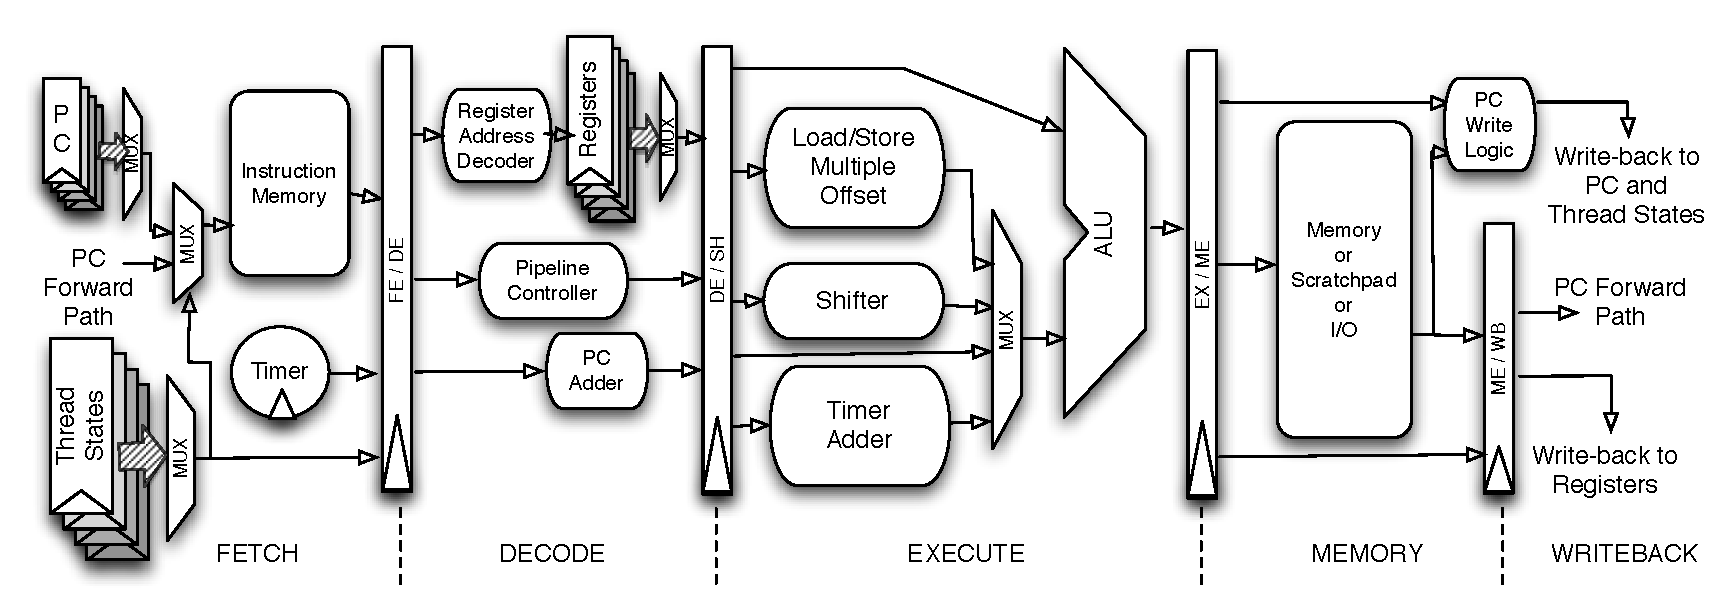
\includegraphics[scale=.54]{figs/ptarm_pipeline_five_stage}
  \end{center}
  \vspace{-20pt}
  \caption{Block Level View of the PTARM 5 stage pipeline}
  \label{fig:ptarm_pipeline_five_stage}
\end{figure}

%The \emph{fetch} and \emph{decode} stages setup the data operands and control signals for the later stages to execute the instruction.
The \emph{fetch stage} of the pipeline selects the correct PC according to which thread is executing, and passes the address to instruction memory. 
The PC forward path forwards a loaded address from main memory for instructions that load to R15, which causes a branch.
We will discuss the need for the forwarding path below when we describe the \emph{writeback stage}.
A simple $log(n)$ bit upcounter is used to keep track of which thread current to fetch.

The \emph{decode stage} contains the \emph{pipeline controller} which does the full decoding of instructions and sets the correct pipeline signals to be propagated down the pipeline.
Most of ARM instructions are conditionally executed, so the pipeline controller first checks the condition bis to determine whether the instruction is to be executed or not.  
Typically the \emph{pipeline controller} needs to know the current instructions in the pipeline to detect the possibility of pipeline hazards and stall the current instruction.
However,in a thread-interleaved pipeline, other instructions down the pipeline are from threads, thus the controller logic is greatly simplified. 
It simply decodes the instruction to determine the correct signals to send to the data-path and multiplexers down the pipeline.
It does not need to know any information about instructions already in flight. 
A small decoding logic, the \emph{register address decoder}, is inserted in parallel with the controller to decode the register addresses from the instruction bits.  
Typical RISC instruction sets, such as MIPS, set the encoding of instruction bits so the register operands have a fixed location for all instruction types.
However, in the ARM instruction set, certain instructions encode the register read address at different bit locations of the instruction.
For example, ARM data-processing register shift instructions reads a third operand from the register to determine the shift amount.
Store instructions also read a third register to obtain the register value that is stored to memory. 
However, both instructions have different bit locations in the instruction encoding to determine what register to read from.
Thus, a small register address decoding logic is inserted for a quick decoding of the register addresses from the instruction bits.
The \emph{PC Adder} is used to increment the PC.
%FIXME: Talk about the design of the ISA to optimize pipeline implementation, which in our case did not make things easier
The ARM ISA programmer's model states that reading from R15 reads the current PC+8, the PC adder not only increments the PC by 4 to get the potential next PC, but it also increments the current PC by 8 to be used as an operand. 
Single threaded pipelines need to increment the PC immediately in the fetch stage to prepare for the next instruction fetch.  
For thread-interleaved pipelines, since the next PC from the current thread is not needed until several cycles later, it doesn't need to be in the fetch stage. 
But because we need the results of PC+8 as a data operand, it is placed in the decode stage. 
The \emph{timer} is a hardware counter clocked to the processor clock which is used to implement the timing instructions mentioned in section~\ref{sec:programming_models}.
The timer contains a 64 bit value that represents nanoseconds, and starts at 0 when the pipeline starts up.  
The time value is latched in the decode stage as the subsequent stages use it for timer manipulation.

The \emph{execute}, \emph{memory} and \emph{writeback} stages execute the instruction and commits the result. 
The \emph{execute} stage contains mostly execution units and muxes that select the correct operand and feeds it to the ALU.  
The ARM ISA assumes a built in shifter to shift the operands before operations, so a 32 bit \emph{shifter} is included to shift the operands before the ALU.   
The \emph{load/store multiple offset} logic block is used to calculate the offset of load/store multiple instructions.
The load/store multiple instruction uses a 16 bit vector to represent each of the 16 general purpose registers.
The bits that are set in that bit vector represents a load/store on that register.
The an offset is added to the base memory address for the instruction, and that offset depends on how many bits are set. 
Thus, the load/store multiple offset logic block does a bit count on the bit vector and adjusts the offset to be passed into the ALU for load/store multiple instructions.
The \emph{timer adder} logic block is a 32 bit add/subtract unit.
Time in the pipeline is a 64 bit value representing nanoseconds. 
Thus, any timing instruction that interacts with the timer in the pipeline needs to operate on 64 bit values.
We could have reuse the existing ALU at the expense of having all timing instructions take an additional pass through the pipeline.
But we chose to include an addition add/subtract unit specifically for the implementation of the delay\_until instruction so it can check for deadline expiration every cycle, which we will discuss in detail in section~\ref{sec:ptarm_instructions} when we show how delay\_until is implemented.    
A 32 bit \emph{ALU} does most of the logical and arithmetic operations, including data-processing operations and branch address calculations.
The results is passed to the \emph{memory stage}, which either uses it as an address to interact with the data memory, or forwards it along to the \emph{writeback stage} to commit back to the registers.

\begin{wrapfigure}{r}{0.5\textwidth}
  \vspace{-20pt}
  \begin{center}
    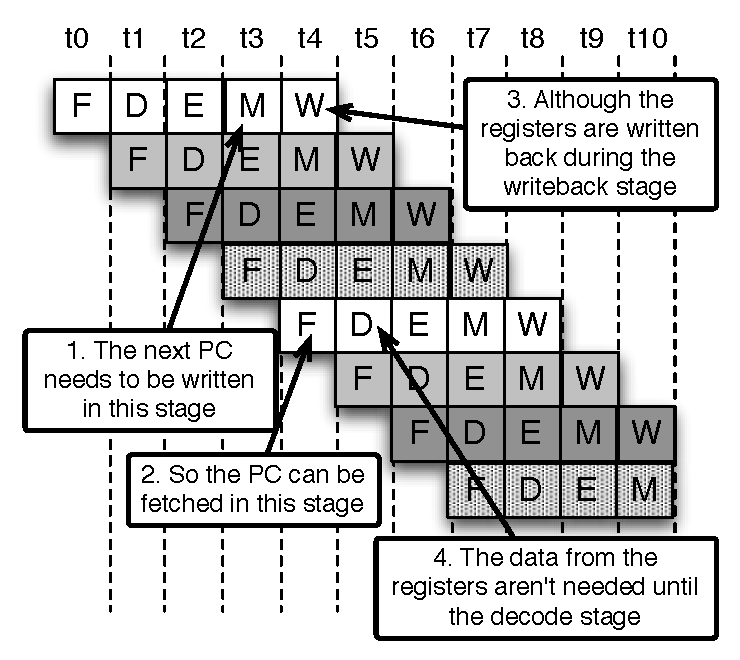
\includegraphics[scale=.65]{figs/four_thread_pipeline}
  \end{center}
  \vspace{-20pt}
  \caption{Four thread execution in PTARM}
  \label{fig:four_thread_pipeline}
  \vspace{-10pt}
\end{wrapfigure}      
%Although the register values are committed in the write back stage, the next PC address needs to be written back earlier. 
Figure~\ref{fig:four_thread_pipeline} shows an execution sequence of the four thread five stage pipeline.
The instruction in the fetch stage belongs to the same thread as the instruction in the writeback stage.
This does not cause any data hazards because the data from the registers will not be read until the decode stage. 
But committing the PC at the writeback stage would result in a control hazard because the PC would not be ready for the subsequent fetch.
For most instructions, the next PC calculation is completed before the memory stage, so we move the PC commit one stage earlier so the next instruction can be fetched.
However, the ARM ISA allows instructions to write to register 15 (PC), which acts as a branch to the value written to R15.   
This means a load instruction can write to R15 and cause a branch whose target is not known until after the memory read.   
Thus, a PC forwarding path is added to forward the PC back from memory if a load instruction writes to R15.  
The forwarding path does not cause any timing analysis difficulties because the statically the forwarding path is only used when a load instruction writes to R15, which can be statically determined. 
Also, this causes no stall in the pipeline, and does not effect the timing of any following instructions. 
This allows us to interleave four threads in our five stage pipeline instead of five.    

\section{Memory Hierarchy}
\label{sec:ptarm_memory}

%Remention why we expose the memory hierarchy to the programmer
%talk about the scratchpad access regions and what memory address they are mapped to
%talk about the front end implementation to access the ptarm memory controller, and the access latencies that is generated   
%talk about the I/O memory region, and how the protocol is implemented to determine if memory access is completed yet

\begin{wrapfigure}{r}{0.5\textwidth}
  \vspace{-20pt}
  \begin{center}
    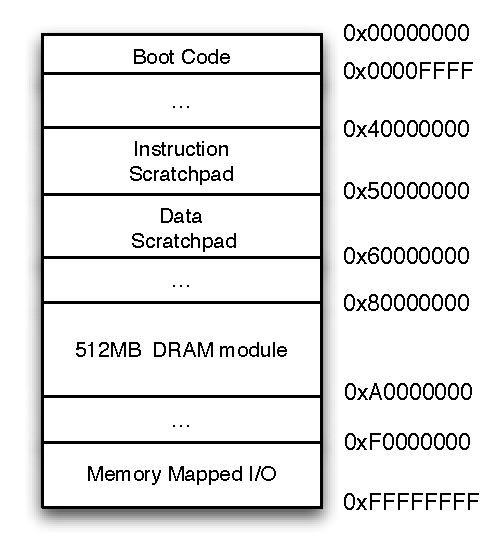
\includegraphics[scale=.65]{figs/ptarm_memory_layout}
  \end{center}
  \vspace{-20pt}
  \caption{Memory Layout of PTARM}
  \label{fig:ptarm_memory_layout}
  \vspace{-10pt}
\end{wrapfigure} 
The memory hierarchy of PTARM is exposed to the programmer, as discussed in section~\ref{section:memory_system}.
It is composed of a boot ROM (read only memory), instruction and data scratchpads, the predictable DRAM controller, and a memory mapped I/O region, all occupying separate address spaces.
Figure~\ref{fig:ptarm_memory_layout} shows the address regions occupied by each memory type.  

\subsection{Boot ROM}
The boot ROM \todo{mention boot code size} contains the reset instructions and exception vector table that stores entries for handling different exceptions that occur in the pipeline.
It also contains shared exception handlers and initialization code. 
The instructions store on the boot ROM cannot be modified at run-time, hence the read-only memory name. 
However, a dedicated region in the boot ROM stores a table for user-registered exception handlers, these entries can be modified prorammatically. 
We use this region to allow users to register timer expire exception handlers.
  
\subsection{Scratchpads}  
The instruction and data scratchpad \todo{size?} can be partitioned into private regions for each thread, or shared by all threads.
If PTARM is used in embedded security application, such as running encryption algorithms on it, then the partitioning the scratchpads into private regions might be desired. 
In chapter~\ref{chapter:app} we will discuss the security implications and how a Precision Timed Machine can defend against side-channel attacks.
On the other hand, sharing the scratchpad could provide flexibility on the allocation of scratchpads between hardware threads.
More space could be allocated to hardware threads running more memory intensive tasks while less could be allocated to the other hardware threads~\todo{cite scratchpad allocation paper}.
%The shared memory space in our system between hardware threads is also allocated on the data scratchpad, because the DRAM controller contains privatized bank resources, and does not allow
%FIXME: separate region for shared scratchpad space?
Both the boot ROM and scratchpads are synthesized to dual-ported block RAMs on the FPGA, and provide deterministic single cycle access latencies.

\subsection{DRAM}
\begin{wrapfigure}{r}{0.5\textwidth}
  \vspace{-20pt}
  \begin{center}
  	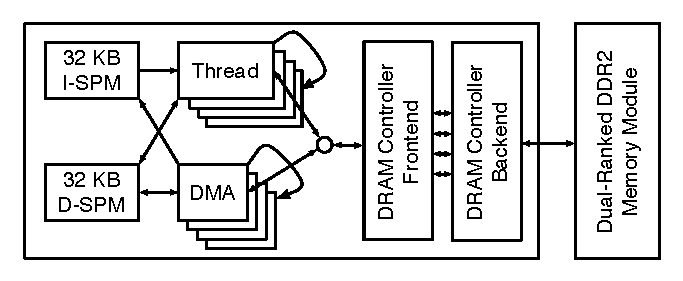
\includegraphics[scale=.6]{figs/pret-integration}
  \end{center}
    \vspace{-20pt}
  \caption{\small{Integration of PTARM core with DMA units, PRET memory controller and dual-ranked DIMM~\cite{ReinekeLiuPatelKimLee11_PRETDRAMControllerBankPrivatizationForPredictability}.}}
\label{fig:pretintegration}
  \vspace{-10pt}
\end{wrapfigure}
All access to the DRAM goes through the predictable DRAM controller described in section~\ref{sec:pret_dram_controller}.
The DRAM controller privatizes the DRAM banks into four resources, which we assign to each thread in our pipeline. 
This removes bank access conflicts and gives us predictable memory access latencies to the DRAM.
The pipeline interacts with the frontend of the DRAM controller, which routes requests to the right request buffer in the backend and manages the insertion of row-access refreshes to ensure the refresh constraint is met.   
In conventional memory architectures where the hierarchy is hidden, the processor interacts with DRAM indirectly by the filling and writing back of cache lines.
In our memory system, the processor can directly access the DRAM through load and store instructions to the distinct memory regions of the DRAM.
In addition, each hardware thread is also equipped with a direct memory access (DMA) unit, which can perform bulk transfers between the scratchpads and the DRAM.
Figure~\ref{fig:pretintegration} shows the integration of PTARM with the DMA units, memory controller and DRAM.  

\begin{wrapfigure}{r}{0.5\textwidth}
  \vspace{-25pt}
  \begin{center}
  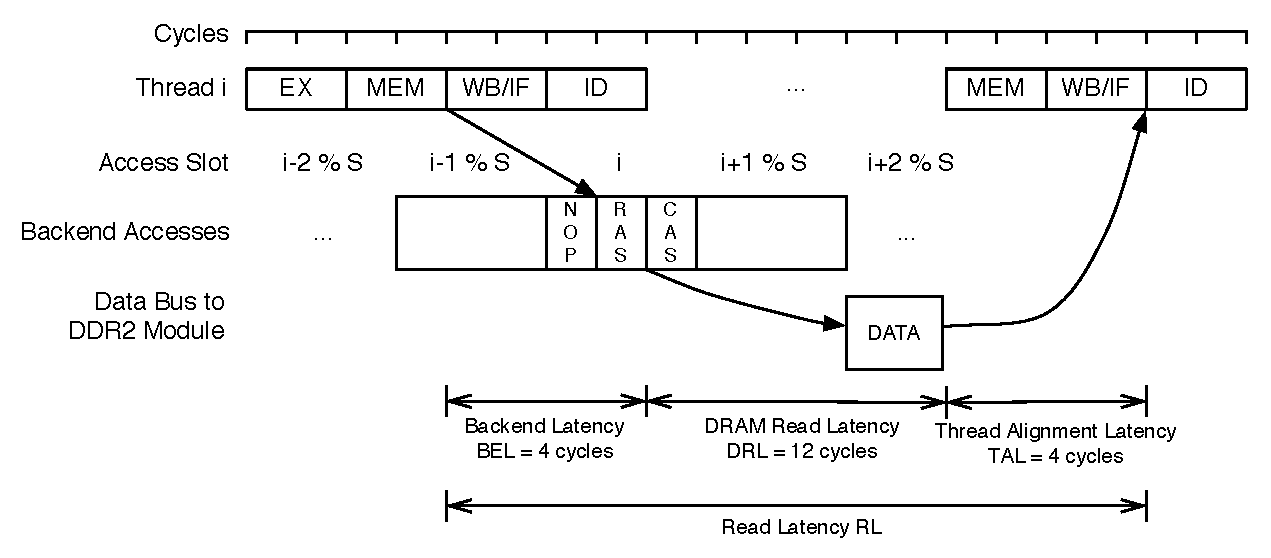
\includegraphics[scale=.38]{figs/readlatency}
  \end{center}
  \vspace{-20pt}
  \caption{\small{Example of a load operation by hardware thread $i$ in the thread-interleaved pipeline.}}
  \label{fig:readlatencyderivation}
\end{wrapfigure}
When DRAM is accessed through load (read) and store (write) instructions, the memory requests are issued directly from the memory stage of pipeline.
The request is received from the frontend of the memory controller, and placed in the correct request buffer. 
Depending on the alignment of the pipeline and the backend, it takes a varying number of cycles until the backend generates corresponding commands to be sent to the DRAM module.
After the read has been performed by the DRAM and has been put into the response buffer, again, depending on the alignment of the pipeline and the backend, it takes a varying number of cycles for the pipeline to reach the write-back stage of the corresponding hardware thread, which picks up the response. 
Figure~\ref{fig:readlatencyderivation}, illustrates the stages of the execution of an example read instruction in the pipeline.
In~\cite{ReinekeLiuPatelKimLee11_PRETDRAMControllerBankPrivatizationForPredictability} we derive the access latencies from the alignment and show that it is either 3 or 4 thread cycles.    
We leverage this misalignment of the pipeline and backend to hide the refresh latency from the front end. 
When a refresh is scheduled for the DRAM resource, if no memory request is in the request buffer, the refresh is serviced.
As mentioned in section~\ref{sec:pret_dram_controller}, if a refresh conflicts with a pipeline load or store, we push back the refresh till after the load or store. 
In this case, the pushed back refreshes become invisible:   
as the pipeline is waiting for the data to be returned and takes some time to reach the memory stage of the next instruction, it is not able to use successive access slots of the backend, and thus it is unable to observe the refresh at all.

Whenever a DMA transfer is initiated, the DMA unit uses the thread's request buffer slot to service DMA requests to/from the scratchpad. 
Thus, while a DMA transfer is initiated, the thread gives up access to the DRAM to the DMA unit.
During this time, the thread can continue to execute and access the scratchpad regions that is not being serviced by the DMA request. 
This is possible because scratchpads are dual-ported, allowing a DMA unit to access the scratchpads simultaneously as its corresponding hardware thread.
If at any point the thread tries to access the DRAM, it will be blocked until the DMA transfer completes.
Similarly, accesses to the region of the scratchpad which are being transferred from or to will stall the hardware thread\footnote{This does not affect the execution of any of the other hardware threads.}.
Since DMA units are not pipelined, there are no ``alignment losses'', so the DMA units can fully utilize the bandwidth provided by the backend.
The DMA latencies are also derived in ~\cite{ReinekeLiuPatelKimLee11_PRETDRAMControllerBankPrivatizationForPredictability}, and can be predictably be determined by the transfer size. 
Similarly, we skip the first refresh during a DMA transfer and schedule an additional one at the end of the transfer.
This pushes back the refresh of a particular row by at most $60 \cdot 13$ cycles.
%Alternatively, this can be seen as shifting all refreshes, during the DMA transfer, back by $63$ slots or to the end of the transfer.
More sophisticated schemes would be possible, however, we believe their benefit would be slim.
With this refresh scheme, refreshes do not affect the latencies of load/store instructions, and the refreshes scheduled within DMA transfers are predictable so the latency effects of the refresh can be easily analyzed.  

\paragraph{Store Buffer}
Stores are fundamentally different from loads in that a hardware thread does not have to wait until the store has been performed in memory.
By adding a single-place store buffer to the frontend, we can usually hide the store latency from the pipeline.
Using the store buffer, stores which are not preceded by other stores can be performed in a single thread cycle.
By \emph{thread cycle}, we denote the time it takes for an instruction to pass through the thread-interleaved pipeline.
Other stores may take two thread cycles to execute.
A bigger store buffer would be able to hide latencies of successive stores at the expense of increased complexity in timing analysis.

\subsection{Memory Mapped I/O}
Currently PTARM implements a separate I/O bus for communicating with I/O.
The bus is currently shared between all threads.
%Also talk about I/O bus connections and the protocol to determine if data is ready

\section{Exception Handling}
\label{subsec:exception_handling_in_ptarm}
When exceptions occur in a single threaded pipeline, the whole pipeline must be flushed because of the control flow shift in the program. 
The existing instructions in the pipeline become invalid, and the pipeline overwrites the PC to jump to a specified exception handler. 
The ARM ISA specifies seven types of exceptions, and an exception vector table that points the PC to specified handler addresses when those exceptions occur. 
The exception vector table is stored in the BootROM in our implementation.
Exceptions can be triggered by external or internal events that occur in the pipeline, such as an toggling an external interrupt signal or using a software interrupt instruction to trigger the exception programmatically.
But no matter how the exceptions are generated, they must be handled predictably in the pipeline.
 
In the context of a thread interleaved pipeline, all threads are temporally isolated. 
Thus, an exception that occurs on one thread must not effect the execution of other threads in the pipeline.
In our pipeline, any exceptions or interrupts that occur during execution are latched at each stage and propagated down the pipeline with the instruction. 
An instruction flush signal is toggled to ensure that this instruction does not commit any state to memory or registers. 
The exception type is checked at the memory stage in the PC write logic before the next PC is committed.  
According to the exception type, the program state register bits are set, and the PC is redirected to the correct entry in the exception vector table. 
The current PC is passed on to the writeback stage to store in the link register (R14).
This provides a mechanism for the program return to the initial instruction where the exception occurs and re-execute it if desired, since the instruction did not complete its execution.
If the exception is generated from after a memory access and detected in the writeback stage, the PC forwarding path is used to fetch the exception vector entry for data memory exceptions. 
Note that it is up the each exception handler to save the register states and stack of the program.  

\begin{wrapfigure}{r}{0.5\textwidth}
  \vspace{-20pt}
  \begin{center}
    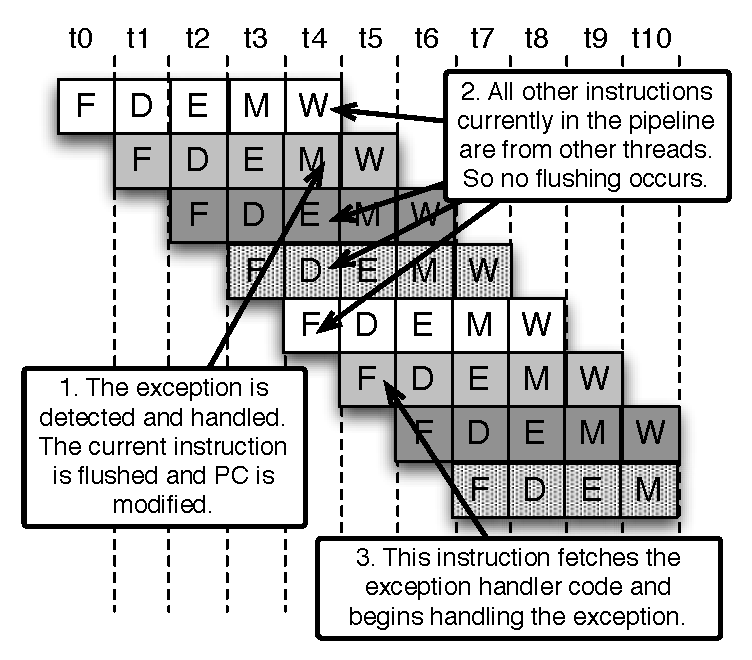
\includegraphics[scale=.65]{figs/exception_handling_pipeline}
  \end{center}
  \vspace{-20pt}
  \caption{Handling Exceptions in PTARM}
  \label{fig:exception_handling_pipeline}
  \vspace{-10pt}
\end{wrapfigure} 
None of the instructions that are executing in the pipeline are flushed when an exception occurs in our pipeline. 
As shown in figure~\ref{fig:exception_handling_pipeline}, the instructions that are executing in other pipeline stages all belong to other threads, so no flushing of the pipeline is required because no instruction was executed speculatively.
This simplifies the timing analysis of exceptions in our pipeline, as the timing behavior of other threads in the pipeline are unaffected.
For the thread which the exception occurs, the only overhead to handling the exception is that the current instruction does not complete its execution this thread cycle.  
The next thread cycle the pipeline will be handling the exception already, resulting in no additional stalls for the thread.

It is possible that an exception occurs during a memory access instruction that is waiting for the results from DRAM to complete. 
In this case, because the memory request is also sent to the DRAM controller, and possible already being serviced by the DRAM, we cannot cancel the memory request abruptly.
In the case that the interrupted instruction was a load, we can simply disregard the results of the load, but if the instruction was a store, we cannot cancel the store request that is writing data to the memory.
So it is up to the programmer to disable interrupts before writing to critical memory locations that require a consistent program state.
By interrupting an instruction that is waiting on memory access to complete, we also potentially complicate the interaction with our DRAM controller.
The DRAM controller can only service one request from each thread at a time for predictable performance\todo{elaborate on this?}.
This normally is not an issue because our pipeline does not reorder instructions or speculatively execute while there are outstanding memory requests, but the pipeline waits until the request is finished before continuing execution.
However, if a memory instruction is interrupted, the pipeline flushes the current instruction and continues execution of the exception handler in the Boot ROM.
If at this point, the exception handler contains a memory request instruction to the DRAM, a memory request would be issued to the DRAM controller that is still servicing the previous request prior to the exception from this thread.
The current memory request in this case would need to wait until the previous ``canceled'' memory request to complete its service by the DRAM before it can begin being serviced.
This creates timing variability to the load instructions because the execution time of load instructions would be different depending on whether an exception just occurred or not.
Because this situation can only occur in the exception handler, because it contains the instructions executed right after an exception, so we leave it to the compiler to ensure that the first few instructions in the exception handler code does not access the DRAM memory region.
In PTARM, the compiler simply needs to ensure that the first three instructions executed from an exception handler are not instructions that access the DRAM.

Currently PTARM does not implement an external interrupt controller to handle external interrupts. 
But when implementing such an interrupt controller, each thread should be able to register specific external interrupts that it handles.
For example, we might have a hard real-time task that is executing on one thread, while another thread without timing constraints is executing on another thread waiting for an interrupt to signal the completion of a UART transfer.
In this case the thread running the hard real-time task should not be effected even if it is in execution when the interrupt occurs.
Only the specific thread handling the UART transfers should be interrupt by this interrupt.  
So we envision an interrupt controller that allows each thread to register specific interrupts that it handles, without affecting other threads in the pipeline.  
%FIXME: Compare to XMOS style handling of interrupts?

\section{Instruction Implementations}
\label{sec:ptarm_instructions}
In this section we go into more details on how each instruction type is implemented and how each hardware block in the pipeline shown in figure~\ref{fig:ptarm_pipeline_five_stage}. 
We will go through different instruction types and discuss the timing implications each instruction in our implementation.
%FIXME: Talk about the difference between thread cycle and regular processor cycle
We will summarize with a table with all instructions and the cycle count it takes to execute them.
   
\subsection{Data-Processing}
We begin by explaining how data-processing instructions are implemented.
These instructions are used to manipulate register values by executing register to register operations. 
Most data-processing instructions take two operands.
One operand is always a register value, the second operand is labeled the shifter operand. 
The shifter operand could be an immediate value or a register value, both which can be shifted to form the final operand that is fed into the ALU.
Figure~\ref{fig:data_processing_pipeline_implementation} explains how data-processing instructions are executed through the pipeline.

\begin{figure}
  \vspace{-20pt}
  \begin{center}
    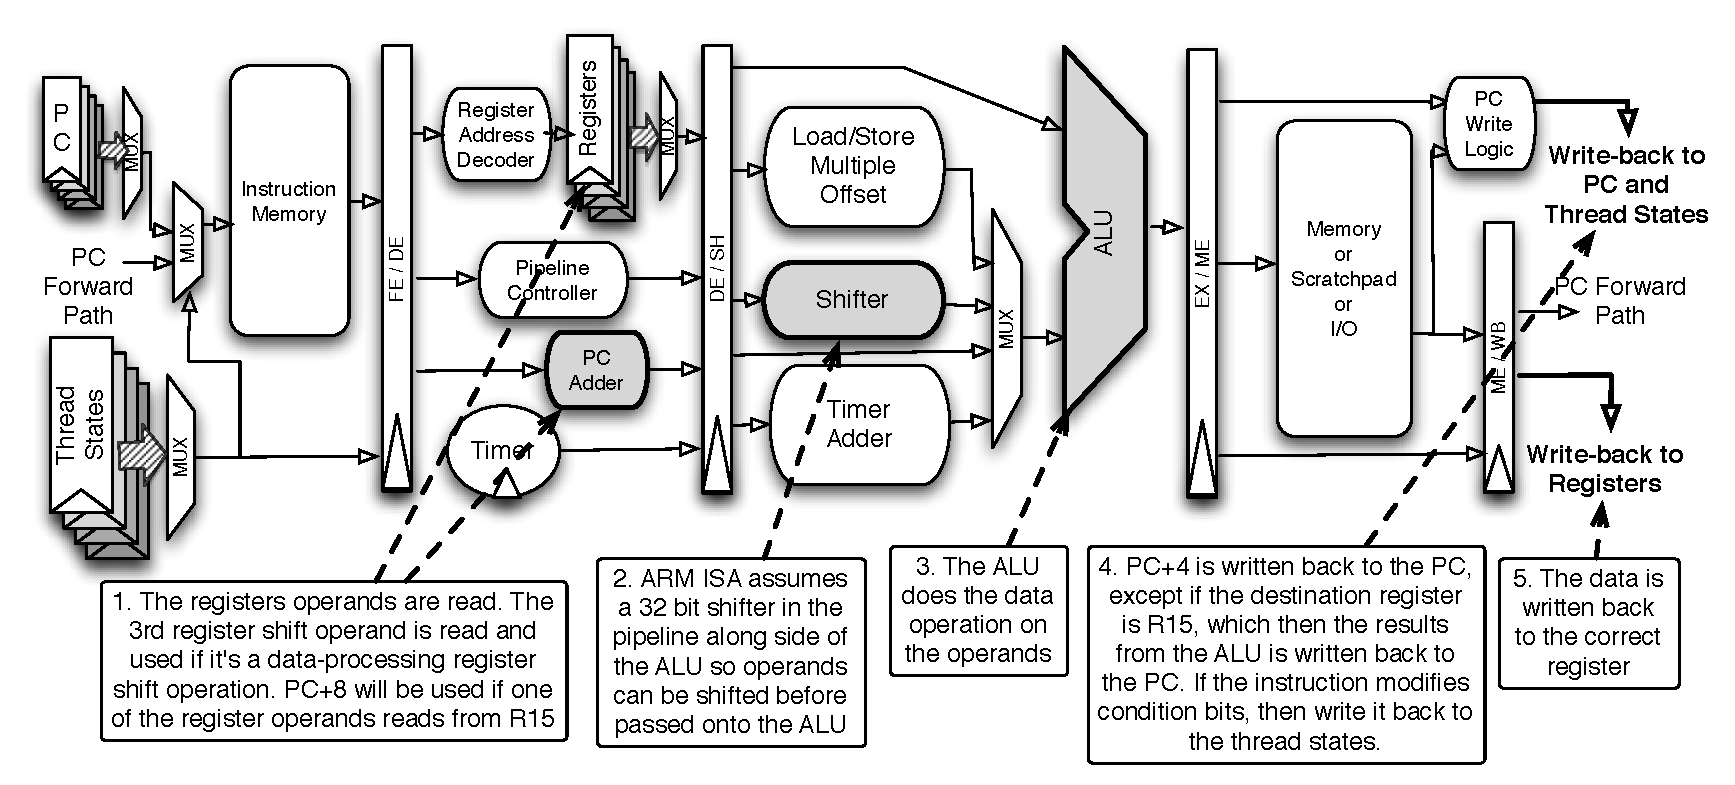
\includegraphics[scale=.54]{figs/data_processing_pipeline_implementation}
  \end{center}
  \vspace{-20pt}
  \caption{Data Processing Instruction Execution in the PTARM Pipeline}
  \label{fig:data_processing_pipeline_implementation}
\end{figure}

Because R15 is PC, so data-processing instructions that use R15 as an operand will read the value of PC+8 as the operand. 
Any instruction that uses R15 as the destination register will trigger a branch to the result of the computation.
As discussed earlier, our pipeline commits the next PC in the memory stage, so to trigger a branch from data-processing instructions simply means storing back the results from the ALU as the next PC.
In our thread-interleaved pipeline, when the next PC from the current thread is fetched, it will contain already contain the target address to branch to when we issue a data-processing instruction that writes to R15. 

Data processing instructions can also update the program condition code flags that are stored in the thread state. 
The condition code flags are used to predicate execution for ARM instructions, and consists of four bits: Zero (Z), Carry (C), Negative (N) and Overflow (V). 
The high four bits of each instruction forms a conditional field that is checked against the thread state condition code flags to determine whether or not the instruction is executed. 
The conditional execution for each instruction is checked in the pipeline controller. 
Data-processing instructions provide a mechanism to update the condition code flags according to the results of data operations.
The instructions that update the flags do not write any data back to the registers, they simply update the condition code flags.

All data-processing instructions only take one pass through the pipeline, even instructions that read from or write to R15, so all data-processing instructions take one thread cycle to execute. 
\subsection{Branch}
Branch instructions in the ARM can conditionally branch forward or backwards by up to 32MB.
There is no explicit conditional branch instruction in ARM.
Conditional branches are implemented using the ARM predicated instruction mechanism.
So the condition used to determine if a conditional branch is taken is simply the condition code flags in the thread state. 
Figure~\ref{fig:branch_pipeline_implementation} show how branch instructions are executed in the thread-interleaved pipeline.

\begin{figure}
  \vspace{-20pt}
  \begin{center}
    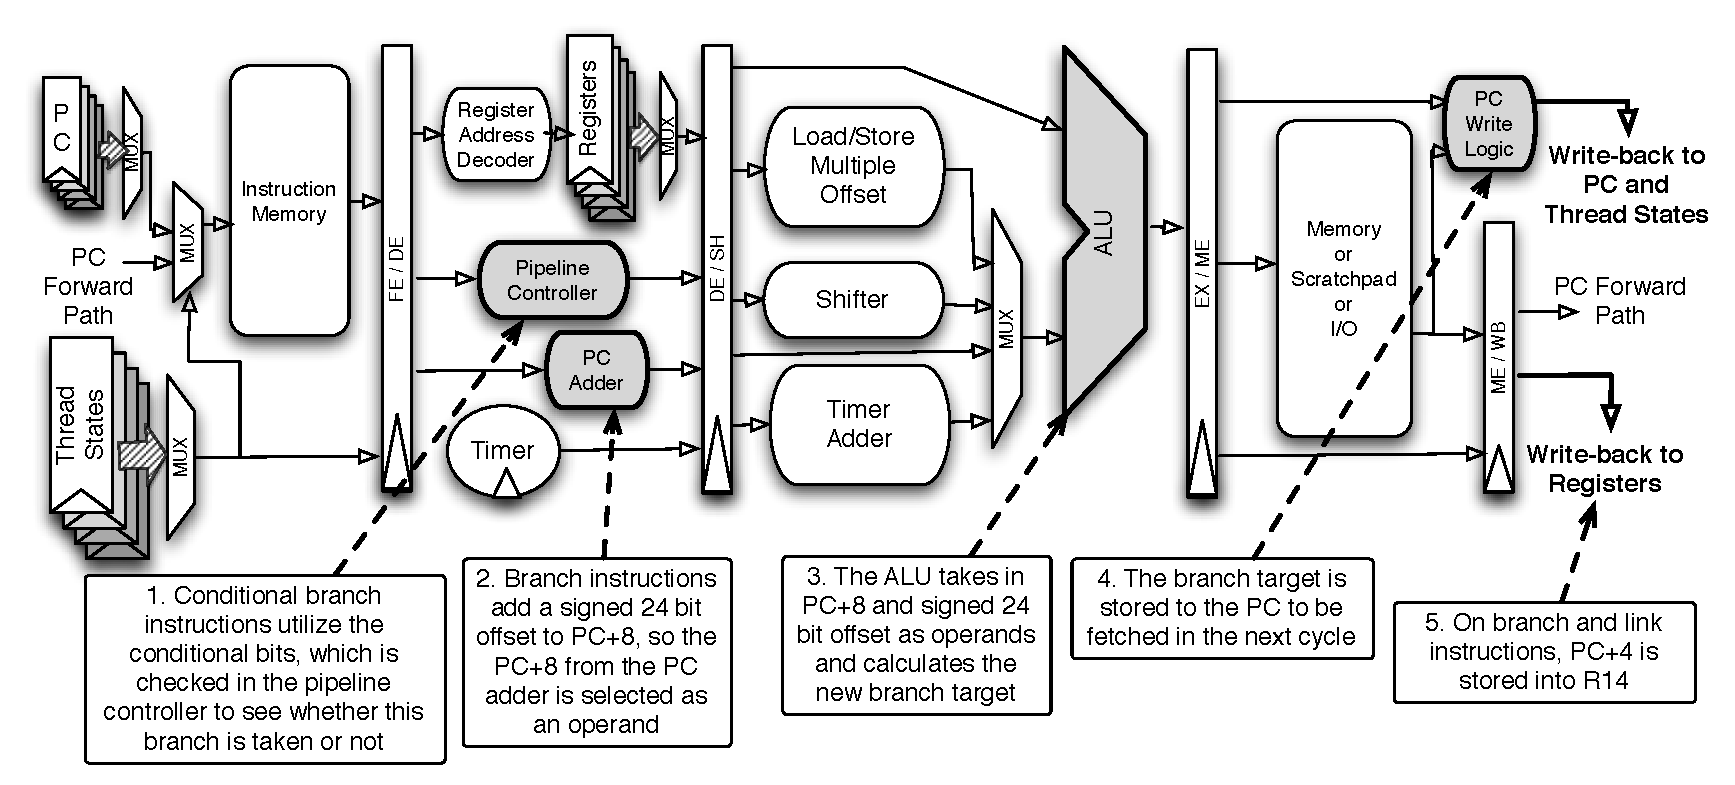
\includegraphics[scale=.54]{figs/branch_pipeline_implementation}
  \end{center}
  \vspace{-20pt}
  \caption{Branch Instruction Execution in the PTARM Pipeline}
  \label{fig:branch_pipeline_implementation}
\end{figure}

The branch instructions for the ARM ISA calculate the branch target address by adding a 24 bit signed offset, specified in the instruction, to the current PC incremented by 8. 
Thus, the PC adder, in addition to incrementing the PC by the conventional offset of 4, also increments the PC by 8, to be used as an operand for the ALU to calculate the target branch address.
Once the address is calculated, it is written back to its thread's next PC ready to be fetched. 
If the instruction is a branch and link ($bl$) instruction, PC+4 is propagated down the pipeline and written back to the link register (R14).   

All branch instructions, whether conditionally taken or not, all take only one thread cycle to execute.
But more importantly, the next instruction after the branch, whether it is a conditional branch or not, is not stalled or speculatively executed. 
The execution time of instructions from the same thread after the branch is not stalled nor affected by the branch instruction.  
The thread-interleaved pipeline simplified the implementation of the branch instruction and control hazard handling logic, as the pipeline will not need the results of the branch target address calculation the very next processor cycle.  
Instead, instructions from other threads will be fetched before the results of the branch is needed.

\subsection{Memory Instructions}
There are two type of memory instructions implemented in PTARM from the ARM ISA: Load/Store Register and Load/Store Multiple.
We discuss both type of memory instructions, and in particular, the interaction of the pipeline with the memory hierarchy presented earlier. 
We also present a special case when the load instruction loads to R15, which loads a branch target address from memory and triggers a branch.  
This slightly complicates our pipeline design, but we show that it does not affect the timing and execution of the instruction and subsequent instructions.
Currently load/store halfword doubleword is not implemented in PTARM, as they fall under the miscellaneous instructions category. 
These instructions can easily be implemented using the same principles described below without significant hardware additions.       
  
\subsubsection{Load/Store Register}
Load instructions load data from the memory and writes them into the registers.
Store instructions store data from the registers into memory, thus store instructions utilize the extra register read port to read in the register value to be stored into memory.
The address used to access memory is formed by combining a base register and an offset value.
The offset value can be a 12 bit immediate supplied from the instruction, or a register operand that can be shifted.
The current load/store instructions can support word operations or byte operations.
Figure~\ref{fig:ldstr_pipeline_implementation} shows how the load/store instruction is executed in the pipeline.

\begin{figure}
  \vspace{-20pt}
  \begin{center}
    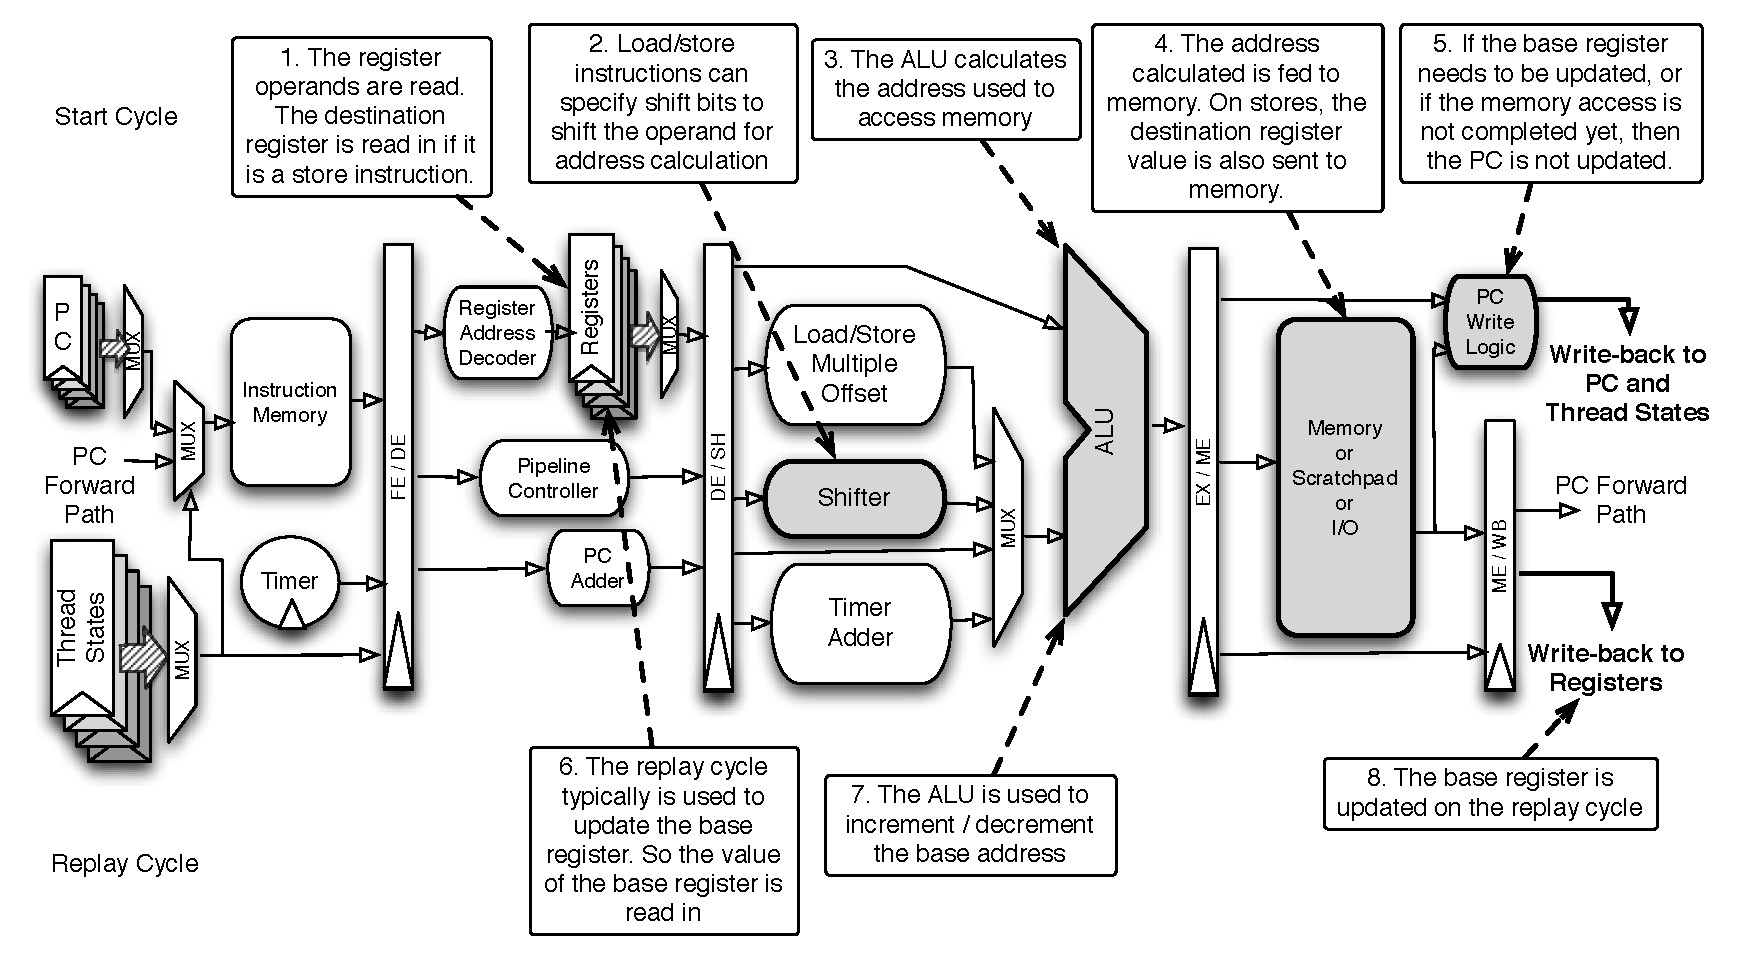
\includegraphics[scale=.54]{figs/ldstr_pipeline_implementation}
  \end{center}
  \vspace{-20pt}
  \caption{Load/Store Instruction Execution in the Ptarm Pipeline}
  \label{fig:ldstr_pipeline_implementation}
\end{figure}

All load and store instructions in ARM have the ability to update the base register after any memory operation. 
This compacts code that reads arrays, as a load or store instruction can access memory and updates the base register so the next memory access is done on the updated base register.
Different address modes differentiate how the base address register is updated. 
Pre-indexed addressing mode calculates the memory address by first using the value of the base register and offset, then updating the base register. 
Post-indexed addressing mode first updates the base register, then uses the updated base register value along with the offset to form the memory address.
Offset addressing mode simply calculates the address from the base register and offset, and does not update the base register. 
The base register could be either incremented or decremented. 
When pre and post-indexed addressing modes are used, memory operations require at least an additional thread cycle to complete.
Because the register file only contains one write port, we cannot simultaneously write back a load result from memory and the updated base register to the register file. 
Thus, we need to spend an extra pass through the pipeline to update the base register.

When the memory address is accessing the scratchpad memory region, memory operations can be completed in a single cycle, and the data is ready by the next (\emph{writeback}) stage to be written back to the registers.
However, if the memory read/write operation is accessing the memory region of the DRAM, the request must go through the DRAM memory controller to access the DRAM. 
%FIXME: update DRAM access latency
DRAM operations typically take three or four thread cycles to complete. 
As discussed in chapter~\ref{chapter:pret}, our thread-interleaved pipeline implementation does not dynamically switch threads in and out of execution when they are stalled waiting for memory access to complete. 
Thus, the when a memory instruction accesses the DRAM memory region, the same instruction is replayed by withholding the update for the next PC, until the data from DRAM arrives and is ready to be written back in the next stage.
For memory instructions accessing I/O regions, the access latency depends on the I/O accessed and the connection of the bus.  
As mentioned in section~\ref{sec:ptarm_memory}, the actual access time to I/O devices is device dependent, and a discussion of time-predictable buses is outside the scope of this thesis.
In the hardware implementation, for memory instructions that access the DRAM or I/O region, it is possible to update the base register earlier during the cycles where the instruction is waiting for access to complete.
However, the current PTARM implementation uses the same logic and datapath for all memory accesses (scratchpad, DRAM, I/O etc) to minimize hardware resources, so an additional cycle is used to update the base register for all memory accesses regardless of the address region they are accessing.

\subsubsection{Load/Store Multiple}
The load/store multiple instruction is used to load (store) a subset, or possibly all, of the general purpose registers from (to) memory.
This instruction is often used to compact code that pushes or pops registers from the program stack.
The list of registers that are used in this instruction is specified in the register list as a 16 bit field in the instruction.
The 0th bit of the bit field representing R0 and the 15th bit representing R15.
A base register supplies the base memory address that is loaded from or stored to, which then is sequentially incremented or decremented by 4 bytes for each register that is operated on. 
Figure~\ref{fig:ldstrm_pipeline_implementation} shows how the load/store multiple instruction is executed in the pipeline. 

\begin{figure}
  \vspace{-20pt}
  \begin{center}
    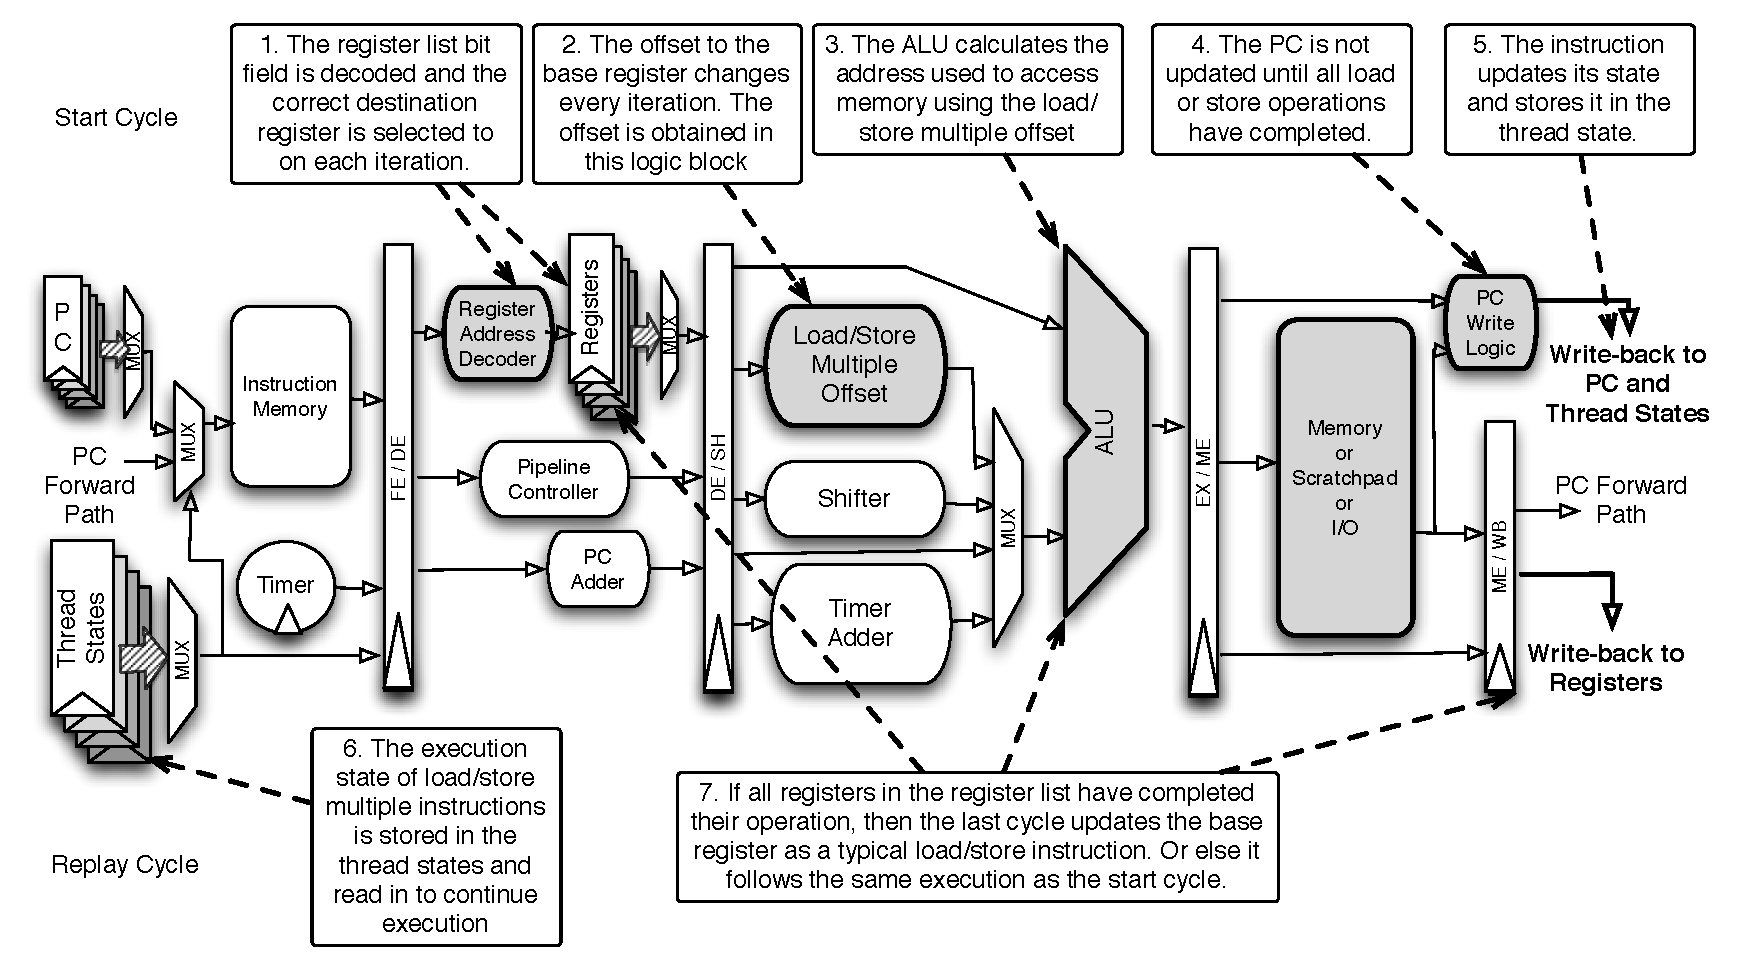
\includegraphics[scale=.54]{figs/ldstrm_pipeline_implementation}
  \end{center}
  \vspace{-20pt}
  \caption{Load/Store Multiple Instruction Execution in the PTARM Pipeline}
  \label{fig:ldstrm_pipeline_implementation}
\end{figure}

The load/store multiple instruction is inherently a multi-cycle instruction, because each thread cycle we can only write back one value to the register or store one value to memory. 
Thus, the execution state and remaining register list of the load/store multiple instruction is stored in thread state.
After the decoding the instruction, the remaining thread cycles load the register field from the thread state and clears it as registers are being operated on. 
The instruction completes when all registers have been operated on.
Each iteration the \emph{register address decoder} in the pipeline decodes the register list and determines the register being operated on.
For load multiple, this indicates the destination register that is written back to.
For store multiple, this indicates the register whose value will be stored to memory.
The \emph{load/store multiple offset} block is used to obtain the current memory address offset depending on how far we are in the execution of this instruction.
The offset is added to the base register to form the memory address fed into memory.

The execution time of this instruction depends on the number of registers specified in the register list and the memory region that is being accessed. 
For accesses to the scratchpad, each register load or store takes only a single cycle. 
However, if memory accesses are to the DRAM region, then register load/store will take multiple cycles.
It is also possible for the load/store multiple instruction to update the base register after all the register operations completes. 
Similar to the load/store register instruction, an additional thread cycle will be used to update the base register.
Although the execution time of this instruction seems to be dynamic depending on the number of registers specified in the register list, but the instruction binary will allow us to statically determine that number by parsing the bit field of the instruction.
Thus, the execution time of this instruction can still be statically analyzed.   

\subsubsection{Load to PC}    
When load/store operations load to the destination register R15, it triggers a branch in the pipeline.
This also holds true for the load multiple instruction if the 15th bit is set in the register list.
In our five stage pipeline, we commit the next PC in the memory stage so the next instruction fetch from the same thread can fetch the updated PC.
However, when the branch target address is loaded from memory, the address is not yet present in the memory stage to be committed, but only at the beginning of the writeback stage will it be present. 
Thus, we introduce a forwarding path that forwards the PC straight from the writeback stage to the fetch stage. 
Figure~\ref{fig:ld_to_pc_pipeline_implementation} shows how this is implemented in our pipeline.   
\begin{figure}
  \vspace{-20pt}
  \begin{center}
    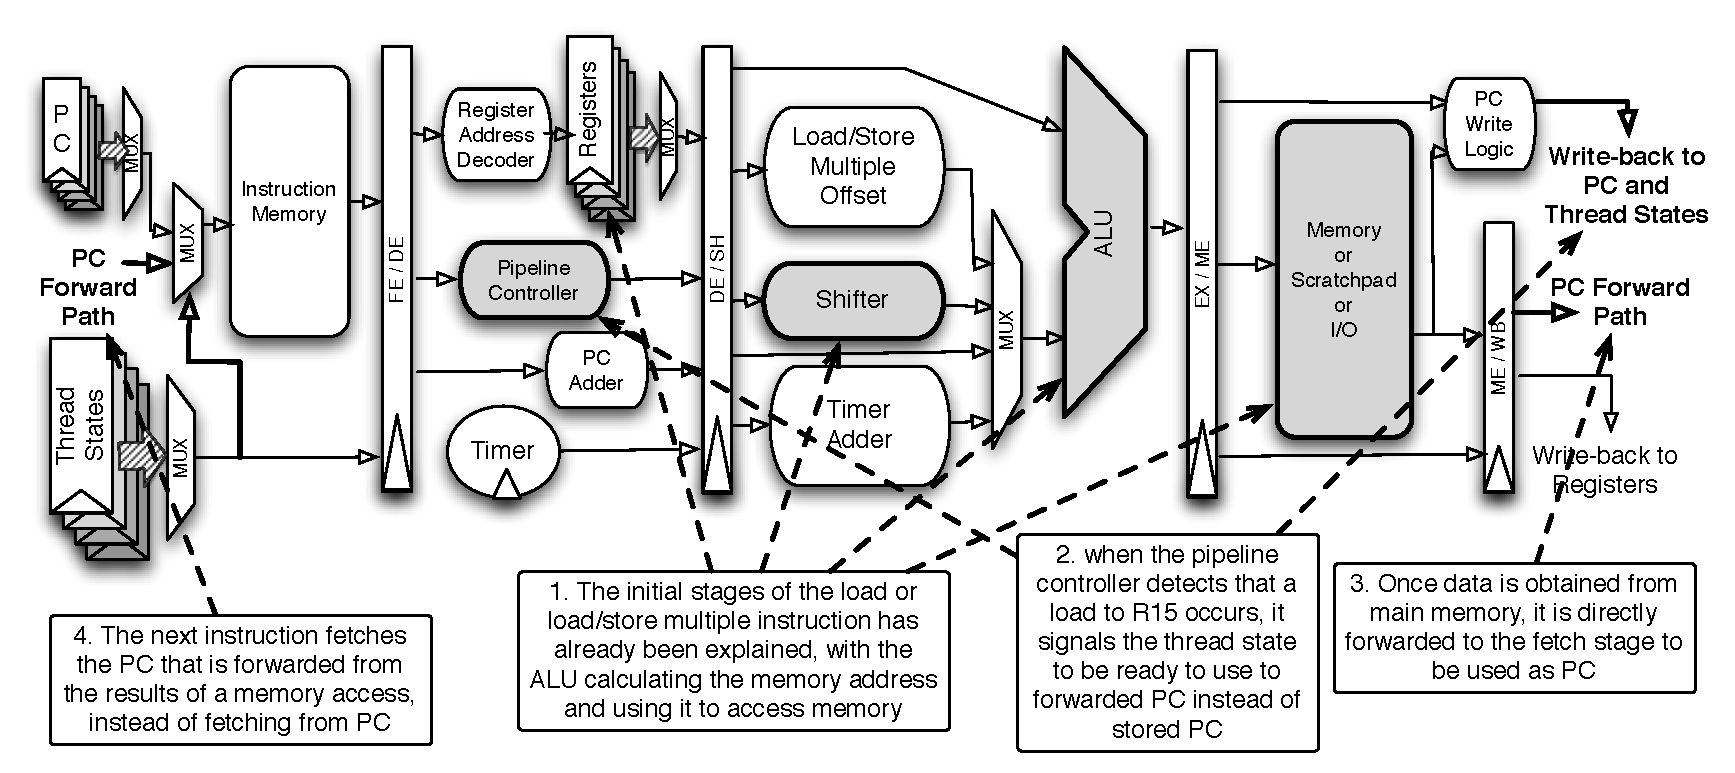
\includegraphics[scale=.54]{figs/ld_to_pc_pipeline_implementation}
  \end{center}
  \vspace{-20pt}
  \caption{Load to R15 Instruction Execution in the PTARM Pipeline}
  \label{fig:ld_to_pc_pipeline_implementation}
\end{figure}

An extra multiplexer is placed in the fetch stage before the instruction fetch to select the forward path.
When a load to R15 is detected, it will signal the thread state to use the forwarded PC on the next instruction fetch, instead of the one stored in next PC.
Because the data from memory will be ready at the beginning of the writeback stage, the correct branch target address will be selected and used.
We discussed in section~\ref{sec:pipeline_hazards} the timing implications of data-forwarding logic in the pipeline.
Those same principles are applied in this situation.
Although it seems the selection of PC is dynamic, but when forwarding occurs is actually static; this PC forwarding only and always occurs when instructions load from memory to R15.
This mechanism has no additional timing effects on any following instructions, as no stalls are needed to wait for the address to be ready. 
Even if the load to R15 instruction is accessing the DRAM region, the timing of this instruction does not deviate from a load instruction destined for other registers.
Although the target address will not be known until after the DRAM access completes, a load instruction that does not load to R15 also needs to wait until the DRAM access completes before the thread fetches the next instruction. 
So this extra forwarding mechanism does not cause load to R15 instructions to deviate from other load timing behaviors.

If the load to R15 instruction updates the base register, then the forwarding path is not used and not needed. 
The extra cycle used to update the base register will allow us to propagate the results from memory to be committed in the memory stage.
The timing behavior still conforms to a regular load to registers instruction. 

\subsection{Timing Instructions}
In section~\ref{sec:programming_models} we presented various instruction extensions to the ISA to bring timing semantics at the ISA level.
We will now present a primitive implementation of those instructions in PTARM.  
ARM provides extra instruction encoding slots to be used to implement instructions for co-processors attached to the core. 
In our case, we implement our timing instructions as part of co-processor 13.
We have already described the functionality and use case of the different timing instructions, table~\ref{table_deadline_insts} shows a summary of the instructions and their op codes.
All instructions have the assembly syntax ``\textbf{\textit{cdp, p13, $<$opcode$>$ rd, rn, rm, 0}}'', with $<$opcode$>$ differentiating the instruction type.
   
\begin{table}
\noindent\makebox[\textwidth]{%
\begin{tabular}{ | l | l | p{6cm} | }
  \hline                        
  Type & Opcode &  Functionality \\ \hline
  \textbf{\textit{get\_time}} & 8  & 
offset = (crm $<<$ 32) + crn; \newline
deadline = \textit{current\_time + offset}; \newline
crd = low32(deadline); \newline
crd+1 = high64(deadline); 
  \\ \hline 
  \textbf{\textit{delay\_until}} & 4 & 
deadline = (crm $<<$ 32) + crn; \newline
if ( \textit{current\_time} $<$ \textit{deadline} )  \newline
\hspace*{5 pt} stall\_thread(); 
 \\ \hline 
  \textbf{\textit{exception\_on\_expired}} & 2 &
offset = (crm $<<$ 32) + crn; \newline
register\_exception(offset);  
\\ \hline
  \textbf{\textit{deactivate\_exception}} & 3 &
deactivate\_exception();  
\\ \hline
\end{tabular}}
\caption{List of assembly deadline instructions}
\label{table_deadline_insts}
\end{table}

The timing instructions uses a master clock to obtain and compare deadlines.
PTARM implements the clock in the \emph{timer} block that is shown in figure~\ref{fig:ptarm_pipeline_five_stage}.   
Time is currently represented as an unsigned 64 bit value with nanoseconds as its units, and starts at zero when PTARM is reset. 
Unsigned 64 bits of nanoseconds can represent time up to approximately 584 years.
\todo{discuss timer implementation relative to different clock speeds. }
Each of the timing instructions operate on 64 bit values, which is stored in two 32 bit registers.
Because the deadlines are stored in general purpose registers, standard arithmetic instructions can be used to manipulate the values. 
However, PTARM does not current provide 64 bit arithmetic operations, so programmers must handle the overflow in software.

For each thread, the timer value is latched into the pipeline at the decode stage, which is where each thread's reference to time is.
Each thread operates on their own private deadlines, and are not affected by the timing instructions from other threads.
PTARM contains 4 hardware threads that are interleaved through the pipeline, so each hardware thread can only access the timer once every 4 processor clock cycles, the granularity of time observed by each thread.
We will discuss the timing implications of this in section~\ref{subsec:precision_timing_inst_ptarm}, in this section we merely present how they  are implemented in the pipeline.
	
\subsubsection{Get\_Time}    
The \emph{get\_time} instruction is used to obtain the current timer value and store it in two general purpose registers.
The \emph{get\_time} instruction also takes two optional source operands to calculate an offset to the current timer value. 
This allows the programmer to obtain the desired deadline time without additional arithmetic instructions.
Figure~\ref{fig:get_time_pipeline_implementation} shows how \emph{get\_time} is implemented in the PTARM pipeline. 
\begin{figure}
  \vspace{-20pt}
  \begin{center}
    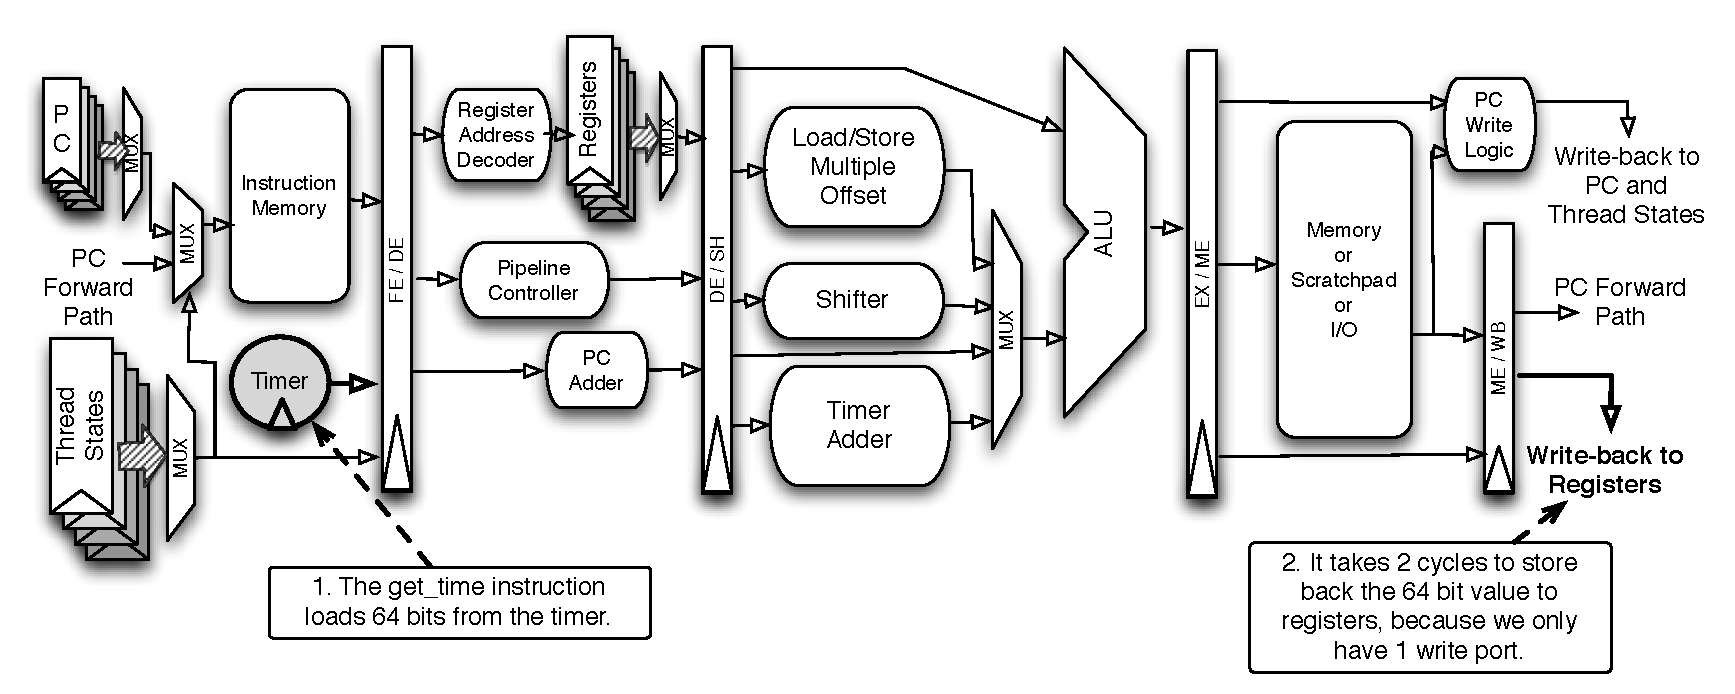
\includegraphics[scale=.54]{figs/get_time_pipeline_implementation}
  \end{center}
  \vspace{-20pt}
  \caption{Get\_Time Instruction Execution in the PTARM Pipeline}
  \label{fig:get_time_pipeline_implementation}
\end{figure}

The timer value and source registers are read in at the decode stage. 
The \emph{timer adder} adds the lower 32 bits of the timer value and source operand while the ALU computes the upper 32 bits taking into account the carry of the \emph{timer adder}.
Once the new deadline has been calculated, it is loaded back into the register file. 
Because our register file only contains one write port, so this instruction also takes two thread cycles to complete; each cycle writes back 32 bits of the new value. 
The calculated 64 bit deadline value is written to the destination register rd and rd+1, with rd storing the lower 32 bits and rd+1 storing the higher 32 bits. 
This instruction will not write to R15 (PC), and it will not cause a branch. 
If R14 or R15 is specified as rd, causing a potential write to R15, then this instruction will simply act as a NOP.

\todo{Talk about whether or not the time passed back adjusts for the latency of the instruction.}

\subsubsection{Delay\_Until}    
\emph{Delay\_until} is used to delay the thread until the a specified deadline has been reached.
It takes in 2 source operands which forms a 64 bit deadline value that is checked against the timer every thread cycle.
The 2 source operands are usually the results of a \emph{get\_time} instruction.  
As described in section~\ref{sec:programming_models}, the \emph{delay\_until} instruction can be used to specify a lower bound execution time for a code block.
This could be useful for synchronization between tasks or communicating with external devices.
Figure~\ref{fig:delay_until_pipeline_implementation} shows the implementation of the \emph{delay\_until} instruction in the PTARM pipeline.       
\begin{figure}
  \vspace{-20pt}
  \begin{center}
    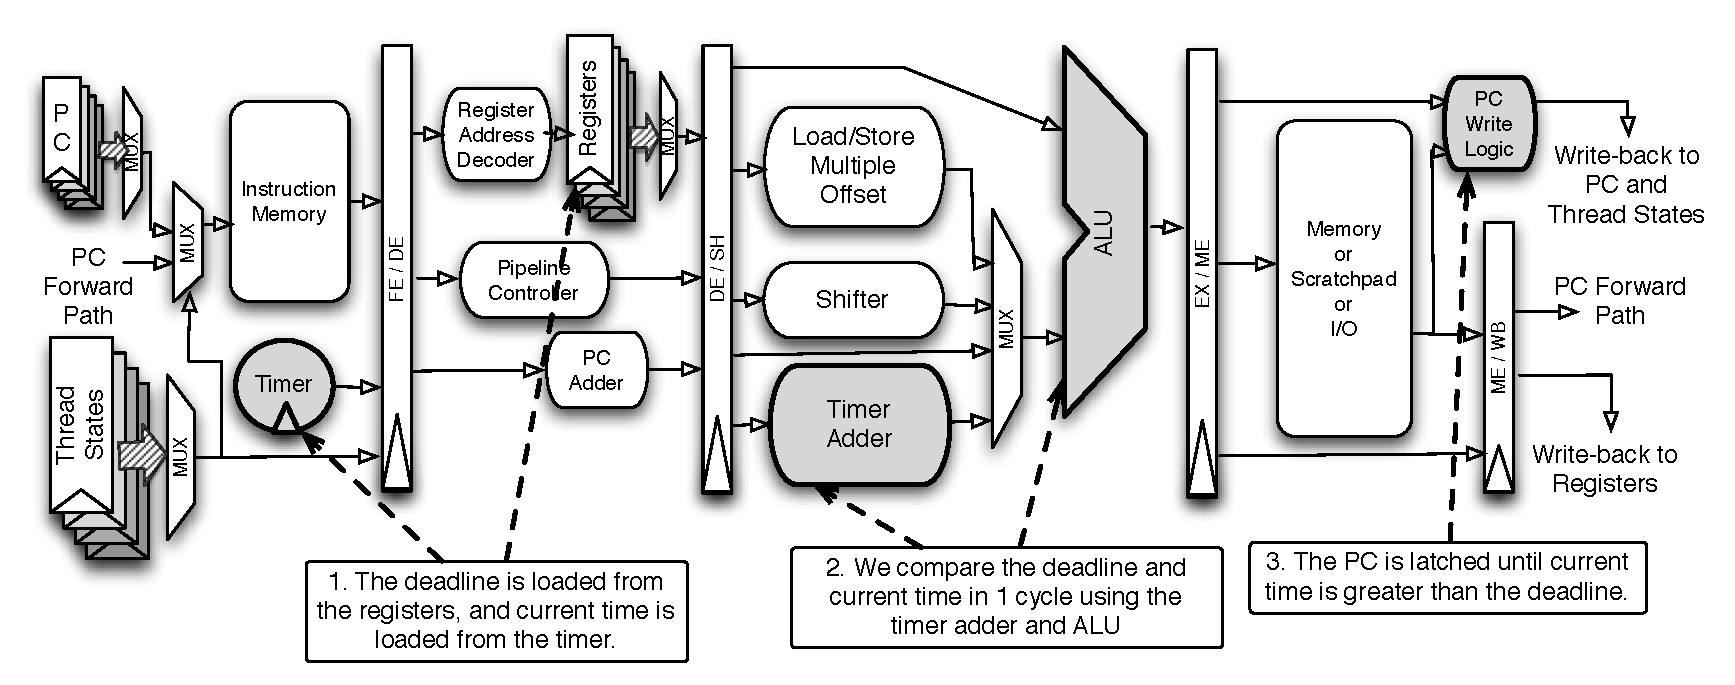
\includegraphics[scale=.54]{figs/delay_until_pipeline_implementation}
  \end{center}
  \vspace{-20pt}
  \caption{Delay\_Until Instruction Execution in the PTARM Pipeline}
  \label{fig:delay_until_pipeline_implementation}
\end{figure}

The implementation of the \emph{delay\_until} instruction is very straightforward, but highlights the reason the \emph{timer adder} is added into the pipeline.
The source operands and the timer value is latched at the decode stage, then compared using the \emph{timer adder} and ALU. 
The next PC is only updated if the timer value is greater than the deadline values passed in.  
Without the additional \emph{timer adder} in the pipeline, comparing 64 bits using our 32 bit ALU would take two thread cycles. 
This would decrease the precision of this instruction by a factor of two, because now we can only check the deadline against the timer every two thread cycles.
The added \emph{timer adder} allows \emph{delay\_until} to check the deadline every thread cycle, to ensure that no additional threads cycles have elapsed right after the deadline is reached. 

\subsubsection{Exception\_on\_Expire and Deactivate\_Exception}    
\emph{Exception\_on\_expire} and \emph{deactivate\_exception} provide a mechanism to actively check for missed code that runs longer than a specified deadline.  
\emph{Exception\_on\_expire} is used to register a deadline for immediate miss detection. 
\emph{Deactivate\_exception} is used to deactivate the active checking before the deadline expires.   
Unlike the \emph{delay\_until} instruction, which checks the deadline when the instruction is decoded, the deadlines registered with \emph{exception\_on\_expire} are checked in hardware in the background. 
A timer expired exception is triggered in the pipeline when a missed deadline is detected.
In section~\ref{sec:programming_models} we have outlines examples of how the instructions are used.

The actual execution of the \emph{exception\_on\_expire} and \emph{deactivate\_exception} instructions is straightforward.    
Within the \emph{timer} unit, there is one 64 bit deadline slot for each thread to register an actively checked deadline.
With four threads in PTARM, there are four slots in the \emph{timer} hardware. 
Whenever an \emph{exception\_on\_expire} instruction is executed, two source operands are read in and stored to the thread's corresponding deadline slot in the \emph{timer}. 
Every clock cycle of the timer, active deadlines are checked against the current timer value.
Once the current timer value surpasses one of the active deadlines, a timer expired exception for the particular thread is raised in the pipeline.
We add an entry to the existing ARM exception vector table to create this timer expired exception. 
The exception is handled the same as any other exception, as discussed in section~\ref{subsec:exception_handling_in_ptarm}, and is only handled by the thread that registered the deadline. 
The other threads in the pipeline remain temporally isolated from this exception.
The execution of a \emph{deactivate\_exception} instruction simply clears the deadline slot for the specific thread.

If threads need to simultaneously check for multiple deadlines, then the single deadline slot for the thread needs to be managed in software.
The software overhead involves managing a list of deadlines and ensuring that the earliest deadline is always being checked in the timer. 
It is possible to implement more than one deadline slot for each thread in the timer if more precise deadline checking is needed. 
However, this comes at the cost of additional hardware complexity in the timer, so currently in PTARM we simply have one deadline slot per thread, and use software mechanisms to manage multiple deadlines in a thread. 

\section{Timing Analysis of PTARM}
\label{sec:wcet}

%mention that a full scaled worst case execution time analysis is beyond the scope of this thesis.
%but do a brief summary on how it's done, cite wilhelm's group's research summary

%give a table of instruction execution

%give more specific examples of exception timing analysis

%give example timiong analysis  
 
\subsection{Precision of timing instructions}
\label{subsec:precision_timing_inst_ptarm}

%discuss the granularity that each thread can obtain with the deadline instructions
%mention that there is no way we can get absolute timing to the finest precision, everything implementation descretizes time 

\section{PTARM VHDL Soft Core}

\begin{wrapfigure}{r}{0.5\textwidth}
  \vspace{-20pt}
  \begin{center}
    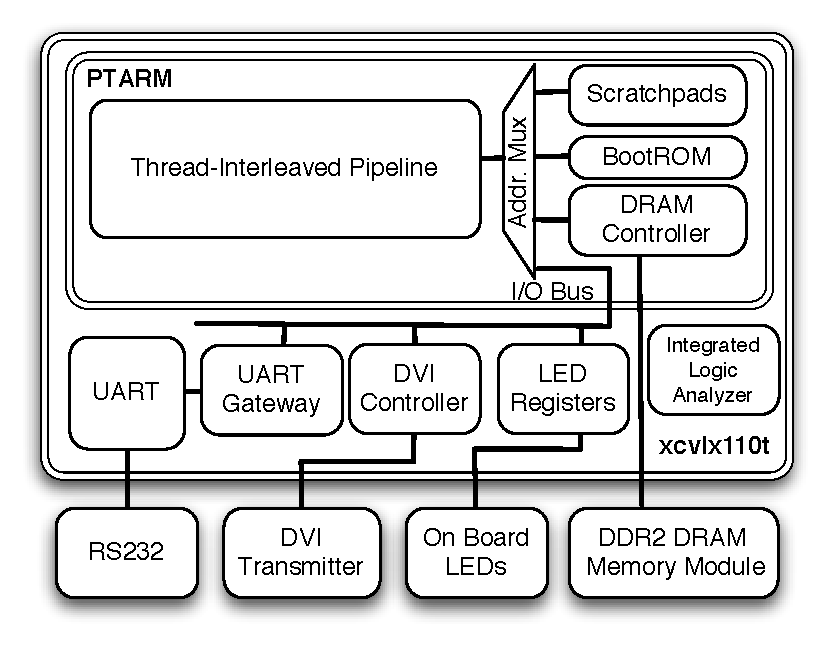
\includegraphics[scale=.6]{figs/ptarm_vhdl_high_level}
  \end{center}
  \vspace{-20pt}
  \caption{PTARM Block Level View}
  \label{fig:ptarm_vhdl_high_level}
  \vspace{-10pt}
\end{wrapfigure}   

Our pipeline can be clocked up to $100MHz$ when synthesized to a Virtex-5 lx110t FPGA.

Figure~\ref{fig:ptarm_vhdl_high_level} shows the high level block diagram of the Softcore.
 
Talk about I/O devices, including UART, DVI controller and Interface with DDR2 DRAM controller

\section{PTARM Simulator}
\label{sec:ptarm_sim}

%Talk about the exploration of DMA memory, and different memory access latencies

Talk about experimentation with DMA and memory hierarchy





\chapter{Applications}
\label{chapter:app}
In this chapter we will present two applications that have been implemented with our Precision Timed Architecture.
The first application is a real-time one dimensional computational fluid dynamics (1D-CFD) simulator.
This simulator runs in real-time to simulate the fuel rail pressure and flow rate for improved engine efficiently when injecting fuel.
The application makes use of the light weight hardware threads in our thread-interleaved pipeline to implement a massively parallel simulator with hundreds of computational nodes communication to its neighbors.
The timing predictable architecture allows us to statically analyze the execution time for each node to ensure that the execution time for each computational node can meet the timing constraints imposed by the application.
A timed base communication scheme is implemented to reduce communication overhead.
The communication synchronization is enforced in software with timing instructions to minimize overhead and enforce that communication occurs on-time and all nodes are in sync.  
We present the synthesis results on a Xilinx Virtex-6 FPGA to show that we can successfully simulate a common fuel rail configuration of up to 234 nodes.       

The second application shows how we use our predictable architecture to eliminate timing side-channel attacks for encryption algorithms.
Time-exploiting attacks take advantage of variations in execution time of cryptosystems to deduce the encryption keys.
The root cause of these time-exploiting attacks is the uncontrollable run-time variance that is caused by the underlying architecture, allowing attackers to bypass the strong mathematical properties of the encryption and deduce the keys.   
We show that by using a timing-predictable architecture that provides more control of execution time to the programmer, we remove the vulnerability that is used to initiate the attack, and remove architecture deficiencies that can lead to more timing-attacks.    
We demonstrate this by running RSA and DSA encryption algorithms on PRET, which successfully illustrates the use of PRET�s timing-centric methods to counter time-exploiting attacks.
 
\section{Real-Time 1D Computational Fluid Dynamics Simulator}
\label{sec:1dCFD}

Modern diesel engines inject diesel fuel with high pressure into the combustion chamber for combustion.
A digital control value is used to control the amount of fuel injected, which depends on the pressure and fuel rate of the fuel rails delivering the fuel.   
Several pilot injections are injected ahead of the main injection to mitigate the inject delay in the chamber and reduce audible noise.
However, these pilot injections send pulsations through the fuel supply rail that need to be modeled or damped before subsequent injection events to ensure the correct amount of fuel is injected~\cite{BoschDiesel}. 
Currently, fuel rails are modeled and developed with 1D-CFD solvers like GT-Fuel, and use an ad-hoc model of fuel pressure for injection events~\cite{Winward01082010}.
1D-CFD models are commonly used in simulating transient operation of internal combustion engines \cite{SAE2009010695}.  
Here, we present an implementation for real-time execution of a 1D-CFD solver using multiple PRET cores that model the fuel rail.
Although the calculations are slightly rougher than the GT-Fuel calculations, it is sufficient to allow improved fuel pressure estimation and close the loop of fuel delivery, allowing for a cleaner, more efficient engine.     


\subsection{Background}
The 1D CFD model of the fuel rail system is descried as a network of pipes.
The system is built up from different types of pipe segments, which each model the fluid dynamics of a segment in the fuel rail.   
A fixed time step solver is implemented.
At each time step, the pipe segments calculate its current pressure and flow-rate, and communicate these to its neighboring pipe segments to be used in the next time step. 
The time step is determined by the speed of information flow that is expressed in equation \ref{Courant}.
\begin{equation} \label{Courant}
\frac{\Delta t}{\Delta x}a = C
\end{equation}
In this equation, \(a\) is the wave speed, \(C\) is the Courant number and \(\Delta x\) is the descretization length.  
For stability, the Courant number needs to be less than 1 and a number below 0.8 is recommended~\cite{GTFuel}.
For example, if a fluid has a wave speed \(a\) of 1 $cm$ per microsecond and a discretization length \(\Delta x\) of 1 $cm$, then we require a time step \(\Delta t\) of less than one microsecond.  
This discretization length of a pipe network is dominated by its smallest sub-volume and a 1 $cm$ discretization length is common for diesel fuel systems.  
For diesel engines, a speed of sound (wave speed) of 1500 $m/s$~\cite{DieselSpeedOfSound} is commonly used.
The real-time requirements of this application thus require adequate performance so that the slowest node can complete in \(\Delta t\).
Although highly parallel, the heterogeneity of pipe elements differentiates this application from typical homogeneous parallel problems often solved using GPUs or SIMD with large common memories~\cite{10.1109/FCCM.2006.20}, such as in image processing applications.

\begin{table}[b]
\begin{center}
\begin{smalltabular}{|l|c|c|}
\hline
\textbf{Type} 							& \textbf{(\emph{Pressure}) $P_{I_n}=$}										& \textbf{(\emph{Flow Rate}) $Q_{I_n}=$} \\ 
\hline
Pipe Segment  						&$\frac{\left(C_P+C_M\right)}{2}$ 				&$ \frac{\left(P_{I_n}+C_m\right)}{B}$ \\ 
\hline
Imposed pressure 							&$\scriptstyle P_{Bnd}$ 							&$\frac{(P_{Bnd}-C_M)}{B}$ \\
\hline
Imposed mass flow  							&$\scriptstyle C_M+BQ_{Bnd}$ 					&$ \scriptstyle Q_{Bnd}$ \\
\hline
\multirow{3}{*}{Valve} 		&\multirow{3}{*}{$\scriptstyle C_P-BQ_{I_n}$}	&$\scriptstyle -BC_V+\sqrt{(BC_V)^2+2C_VC_P}$ \\ 
 								&													&$\scriptstyle C_V=\frac{(Q_0 \tau)^2}{2P_0}$\\ 
\hline
Cap 							&$\scriptstyle C_P-BQ_{I_n}$ 					&$\scriptstyle 0$ \\ 
\hline
\multirow{3}{*}{``T" intersection} 	&\multirow{3}{*}{$\frac{\frac{C_{P_1}}{B_1}+\frac{C_{M_2}}{B_2}+\frac{C_{M_3}}{B_3}}{\sum \frac{1}{B}}$} &$-\frac{P_I}{B_1}+\frac{C_{P_1}}{B_1}$ \\ 
 								&  													&$-\frac{P_I}{B_2}+\frac{C_{M_2}}{B_2}$\\ 
 								& 													&$-\frac{P_I}{B_3}+\frac{C_{M_3}}{B_3}$\\ 
\hline
\end{smalltabular}
\caption{Table of supported pipe elements and their derived equations} 
\label{tab:1dcfd_pipe_types}
\vspace{-8mm}
\end{center}
\end{table}

In order to evaluate our system of pipes we define a few types of computing nodes that corresponding to different pipe elements.
These are shown in table~\ref{tab:1dcfd_pipe_types} with derived pressure and flow rate equations.
From these pipe elements we can generate a network of pipes that represent our fuel system.  
The \emph{imposed pressure} is used to represent the pressure sensor on the fuel system. 
The \emph{imposed mass flow} is used to represent pump, and the \emph{valve} is typically used to represent an injector.
\emph{Pipe segments} and \emph{pipe ``T''} are the interconnected pipe elements, and the \emph{cap} is used to represent the end of a pipe.
The derived equations shown in the table use the following simplified characteristic equations derived in~\cite{viele20121dcfd}.  
\begin{equation}
C_P=P_{i-1}+Q_{i-1}\left(B-R|Q_{i-1}|\right) \text{ and}
\end{equation}
\begin{equation}
C_M=P_{i+1}-Q_{i+1}\left(B-R|Q_{i+1}|\right).
\end{equation}
In the equations, \(B = a\rho / A\) and \( R=\rho f \Delta x/2DA^2\), where \(A\) is the cross sectional area of the pipe, and \(Q\) is the flow rate along the pipe.
\(P\) is pressure, \(\rho\) is fluid density, \(V\) fluid velocity, \(f\) is the Darcy-Weisbach friction factor, \(D\) is pipe diameter, and \(a\) is the wave speed.
The $_{Bnd}$ subscript denotes a boundary condition.  
$C_v$ is the flow coefficient which is a function of: $Q_0$ the nominal open flow, $P_0$ the downstream pressure, and $\tau$ the fraction the valve is open. 
The $_{i+1}$ subscript and $_{i-1}$ subscript represent values that are received from the neighboring pipe elements.
Any implementation of the system must ensure that these calculations for all pipe elements can be completed within the specified time step.
  
\begin{figure}
\noindent\makebox[\textwidth]{
\begin{minipage}[b]{0.55\linewidth}
\centering
\includegraphics[page=22,scale=0.6]{./figs/1dcfd/FCCM2012Figures.pdf}
\caption{Design Flow}
\label{fig:1dcfd_design_flow}
\end{minipage}
\hspace{0.5cm}
\begin{minipage}[b]{0.45\linewidth}
\centering
\includegraphics[page=7, scale=0.5]{./figs/1dcfd/FCCM2012Figures.pdf}
\caption{High Level System Diagram}
\label{fig:1dcfd_HighLevelDiagram}
\end{minipage}
}
\end{figure}

Figure \ref{fig:1dcfd_HighLevelDiagram} shows an overview of a representative system for modeling fuel rails.  
The 1D-CFD model is bounded inside the dashed rectangle.  
External to that is the real-word sensor and actuator interfaces that provide boundary conditions or consume model output variables.  
The small blue squares inside the dashed rectangle represent the network of pipes.  
In a practical simulation of a diesel fuel system the total number of pipe elements can range from around 50 to a few hundred.  
The overall design flow of generating the 1D-CFD model is shown in figure~\ref{fig:1dcfd_design_flow}.
The flow system description describes the fuel rail configuration, which is used to create a graph that describes the system, and determine the system parameters and time step requirements. 
With the graph and library of elements, we instantiate the hardware implementation, then compile and deploy the system. 

For illustrative purposes, we show a sample pipe network graph in figure~\ref{fig:1dcfd-DetailedDiagram}.
Each pipe element is also referred to as a computational node.
Its graphical representation is shown in Table~\ref{tab:1dcfd-CELibrary}. 
%This graph represents the 1D-CFD model that would be implemented within the dashed rectangle in figure~\ref{fig:1dcfd_HighLevelDiagram}.
This pipe network starts with an imposed flow input (P1) element on the left, which represents a pump. 
Fluid travels through a few pipe segment nodes (P2 and P3) to a ``T" intersection (P4), where it splits off to a second branch of the network.
The ``T" node is also measured by the outside world (D1) through a output port.  
Output elements are used when data needs to be communicated out of the model to other parts of the FPGA. 
Flow going up the new leg ends in a cap (P8), while flow continuing down the original path exits the system through a valve (P6).  
{\em Mechanical calculation} elements compute the inputs to valve, defined flow, and defined pressure blocks.
The system is assumed to be at uniform temperature.
Temperature dependent variables like density and wave speed are computed by the global calculation nodes (G1, G2, and G3).
This values are needed by all computational elements in the graph, thus are distributed by the global distributions (GD1, GD2, and GD3) to each of the computational elements every time step.

\begin{figure}
\noindent\makebox[\textwidth]{
\begin{minipage}[b]{0.6\linewidth}
\centering
\includegraphics[page=3, scale=.28]{./figs/1dcfd/FCCM2012Figures.pdf}
\caption{\small{Detailed System Diagram}}
\label{fig:1dcfd-DetailedDiagram}
\end{minipage}
\hspace{0.2cm}
\begin{minipage}[b]{0.4\linewidth}
\centering
\begin{scriptsizetabular}{|p{1.5cm}|c|p{1.5cm}|c|}
\hline
Pipe segment				&\includegraphics[page=11, scale=0.25]{./figs/1dcfd/FCCM2012Figures.pdf} &
Cap 						&\includegraphics[page=12, scale=0.25]{./figs/1dcfd/FCCM2012Figures.pdf} \\ \hline
Imposed pressure 			&\includegraphics[page=13, scale=0.25]{./figs/1dcfd/FCCM2012Figures.pdf} &
Imposed flow 				&\includegraphics[page=14, scale=0.25]{./figs/1dcfd/FCCM2012Figures.pdf} \\ \hline
Pipe ``T" 					&\includegraphics[page=15, scale=0.25]{./figs/1dcfd/FCCM2012Figures.pdf} &
Valve 						&\includegraphics[page=16, scale=0.25]{./figs/1dcfd/FCCM2012Figures.pdf} \\ \hline
Mechanical calculation	&\includegraphics[page=17, scale=0.25]{./figs/1dcfd/FCCM2012Figures.pdf} &
Global calculation 		&\includegraphics[page=18, scale=0.25]{./figs/1dcfd/FCCM2012Figures.pdf} \\ \hline
Global distribution 		&\includegraphics[page=19, scale=0.25]{./figs/1dcfd/FCCM2012Figures.pdf} &
Output 					&\includegraphics[page=20, scale=0.25]{./figs/1dcfd/FCCM2012Figures.pdf} \\ \hline
\end{scriptsizetabular}
\caption{\small{Library of Computational Node Elements}}
\label{tab:1dcfd-CELibrary}
\end{minipage}
}
\end{figure}

\subsection{Implementation}
This application presents several requirements that must be considered when being implemented. 
First, the whole system operates in time steps, which serves as the timing constraints that the longest executed computation node must meet.
Second, communication is exchanged between nodes only once each time step, so synchronization is required between the heterogeneous nodes that exhibit varying execution times.
Third, a typical fuel rail configuration range from fifty to several hundred pipe elements, thus any implementation must be scalable enough to support the larger configurations.
With these requirements in mind, we will detail the implementation of the 1D-CFD simulator with Precision Timed Architectures.

\subsubsection{Hardware Architecture}
\label{sec:1dcfd-hardware_architecture}  
\paragraph{PTARM Cores}
Our hardware implementation synthesizes multiple PTARM cores connected through point-to-point connections on an FPGA.
Computational nodes are each mapped to hardware threads on the PTARM cores.
The PTARM core used for this application is a slightly modified version of the one presented in chapter~\ref{chapter:ptarm}.
In order to improve the throughput and clock frequency of our pipeline, we implemented a six-stage thread-interleaved pipeline shown in figure~\ref{fig:ptarm_pipeline_six_stage}.
 \begin{figure}
  \vspace{-20pt}
  \begin{center}
    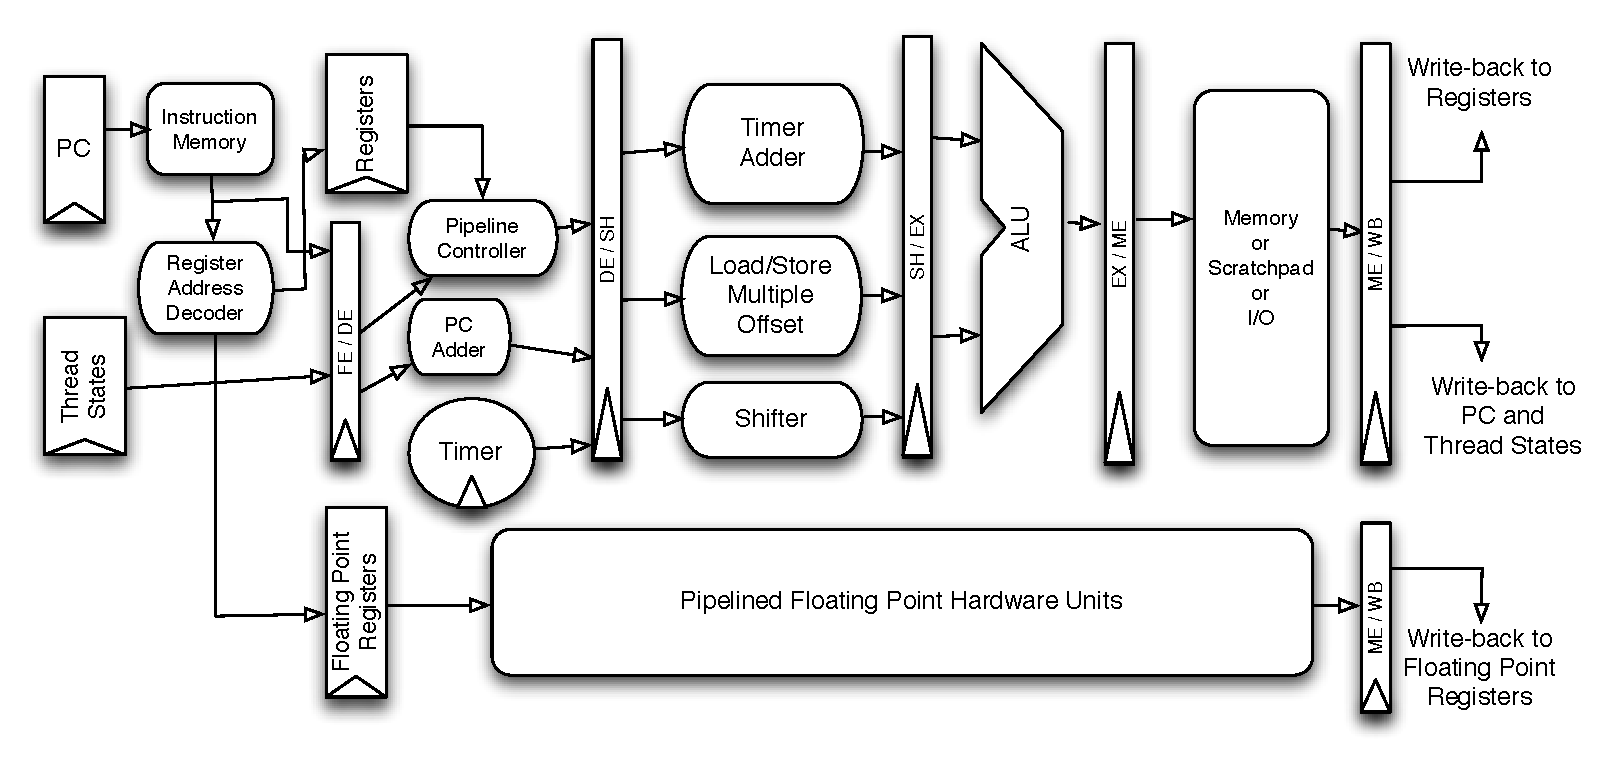
\includegraphics[scale=.54]{figs/ptarm_pipeline_six_stage}
  \end{center}
  \vspace{-20pt}
  \caption{The PTARM 6 Stage Pipeline}
  \label{fig:ptarm_pipeline_six_stage}
\end{figure}
This thread-interleaved pipeline follows the same design principles as discussed in chapter~\ref{chapter:pret}, and supports a minimum of six threads interleaved through the pipeline.
The memory footprint for each of the computational nodes range from roughly 100 to 1000 bytes.  
Thus, scratchpad memories are sufficient to hold all instructions and data for all threads within a PTARM core, no external memory is required. 
The pipeline also contains hardware floating point units to support the applications needs of floating point computations.
The floating point units are single-precision, and generated using the Xilinx Coregen tool~\todo{cite}. 
They are pipelined to accept input every cycle, which avoids structural hazards, as explained in section~\ref{section:pret_thread_pipeline}.   
The floating point operations supported are: add, subtract, multiply, float-to-fix, fix-to-float, divide and square root. 

Our pipeline design supports configurations which exclude certain floating point units, since not all computational nodes require all floating operations.   
For example, square root is only used by the valve node, and divide is only used by the ``T'' node, as shown in table~\ref{tab:1dcfd-inst-count}. 
The floating point divide and square root hardware are the most resource intensive units, but the valve and ``T'' nodes usually represent only a few percent of overall system.
The common fuel rail system we will present later contains 234 nodes, but only 5 nodes are ``T'' nodes and only 4 nodes are valves.
To save on hardware resources, we could use software emulation for the complex operations at the cost of increase the execution time of the ``T'' nodes and valve nodes.
However, the overall performance of our system is bounded by the slowest computational element, because all nodes synchronize communication points at the end of each time step.   
As a result, the performance hit from using software emulation for these small percent of nodes would limit the overall performance. 
Instead, by allowing different configurations of PTARM cores within the system, we can include the hardware additions only on cores that require them, getting the performance boost from hardware without a huge resource overhead.   
This results in substantial resource savings, which we show in section~\ref{sec:1dcfd-results}.

The real-time, highly parallel yet heterogeneous nature of this application makes it a perfect match for our Precision Timed Architecture.
As explained in section~\ref{section:pret_thread_pipeline}, thread-interleaved pipelines contain simpler pipeline architectures, allowing for higher clock frequencies and less resource usage.   
The sharing of the data-path between multiple hardware threads further allows us to optimize the resource usage per computational element.
%We discuss in more details the trade-offs involving adding threads later in section~\ref{sec:1dcfd-results}.
The thread-interleaved pipeline also maximizes throughput over latency, which benefits this highly parallel application.  
The pipeline hide the latencies of multi-cycle operations, such as floating point operations, with execution from other threads.
E.g., in our implementation, the normally 4 processor cycle floating-point additions and subtractions appear as single thread cycle instructions because their latencies are fully hidden by the thread interleaving. 

\paragraph{Interconnect}
\begin{wrapfigure}{r}{0.5\textwidth}
\centering
\includegraphics[page=8, width=0.49\textwidth]{./figs/1dcfd/FCCM2012Figures.pdf}
%\caption{System of Multi-threaded PRET Cores and Interconnects}
\caption{\small{System of PRET Cores and Interconnects}}
\label{fig:1dcfd-hardware}
\vspace{-5mm}
\end{wrapfigure} 
This application requires support for two types of communication.
Between neighboring nodes, the pressure and flow rate values computed are exchanged every time step.
Across the system, several temperature dependent parameters are calculated and broadcast to all nodes every time step as well.
Thus, along with point to point communications between nodes, we also implement a global broadcast circuit.     
Each node can receive up to four inputs and transmit four outputs each time step, depending on the number of neighboring nodes it is connected to.
Out of the inputs, one is dedicated to receiving broadcasts from the global distribution circuit.

Because nodes are mapped to hardware threads on a core, their neighboring node may be mapped to another thread on the same core, or a thread on a neighboring core.  
Nodes mapped to the same core (intra-core communication) communicate through the shared scratchpad memory within the core.
For nodes mapped to different cores (inter-core communication), we use privately shared Block RAMs (BRAMs) between cores to establish the point-to-point communication channel.
BRAMs are dedicated memories on the FPGA that provide single cycle deterministic access latencies, scratchpad memories within each core are also synthesized to BRAMs.
Because the communication bandwidth requirements are small, we only need one shared BRAM between two cores to establish communication channels for all threads on both cores.
This allows all threads to communicate with each other with single cycle latency, whether it is intra-core or inter-core communication.   
As an added benefit, by using BRAMs for communication, we save the logic slices on the FPGA to implement more cores to support bigger models.
On modern FPGAs, the limiting resource factor is typically logic slices, not BRAMs.
Each core only requires a small number of BRAMs to be used for registers and scratchpads, so the BRAM utilization ratio is far less than the logic slice utilization ratio when we synthesize many cores. 
As we present our synthesis results in section~\ref{sec:1dcfd-results}, we will show that the number of cores synthesized is indeed limited by the logic slices, not the BRAMs. 
 
When implementing the global distribution circuit, we observed that only a few nodes are required to the broadcast all the temperature dependent parameters.   
In fact, in diesel fuel systems, the number of nodes needed to broadcast all parameters can be mapped to the six threads of one single PTARM core. 
Thus, we dedicate one PTARM core in the system as the broadcast core.
For each other core, we add a dedicated broadcast receiving memory that is connected to the broadcast core.
The broadcast receiving memory is also synthesized to a small dual-port BRAM, with a read-only port connected to the core, and a write-only port connected to the broadcaster.
The broadcast core contains a broadcast bus that can simultaneously write to all the broadcast memories the same values.
The broadcast memory is also shared amongst all threads in a core so all threads can access the global values. 
This architecture allows us to save on the resources needed to implement a full fledged interconnect routing system or any network protocol to be used for broadcasting. 
Figure~\ref{fig:1dcfd-hardware} shows a block-level view of the hardware architecture.    

%------------------------------------------------------------------------ 
\subsubsection{Software Architecture}
\label{sec:1dcfd-software_architecture}
We implement the equations in table~\ref{tab:1dcfd_pipe_types} in the language C and compile it with the GNU ARM cross compiler~\cite{gnu-arm} to run on our cores. 
In order to minimize the computation required, the equations are statically optimized.  
%Table~\ref{tab:1dcfd-inst-count} show the number of multiply, add/subtract, absolute value, square root, and divide operations required by each computational node after optimization.
The communication channels in and out of each node is memory mapped to the shared BRAMs between cores.

The execution of the system progresses in time steps.  
Computational nodes have varying execution speeds, to avoid data races and ensure all communication is synchronized each time step, we enforce an execution model where each time step consists of several synchronized phases, as shown in figure~\ref{fig:1dcfd-software_model}.
For pipe nodes that read in neighboring data, shown on the top of figure~\ref{fig:1dcfd-software_model}, the first phase of each time step is to read in pressure and flow rate values from neighboring nodes, and the temperature dependent variables from the global broadcasters.
Once input values are read, the computation occurs according to the specific fluid dynamics equations.
The final phase of each time step, the computed results are posted to be used in the next time step.
For global and mechanical nodes, the two phases consists of reading in external values for calculation, and posting results.
We synchronize the data exchange between nodes to ensure avoid data races and ensure that all data operated on is consistent and from the same time step. 
This communication model is very similar to Giotto~\todo{cite}, where tasks communicate explicitly through ports, and only at the end of execution of the tasks to ensure deterministic communication between the tasks. 
While implementations of Giotto use an explicit run-time system to enforce the execution model~\todo{cite}, we use the timing instructions provided by the PRET architecture to implement our system.   

\begin{figure}
\centering
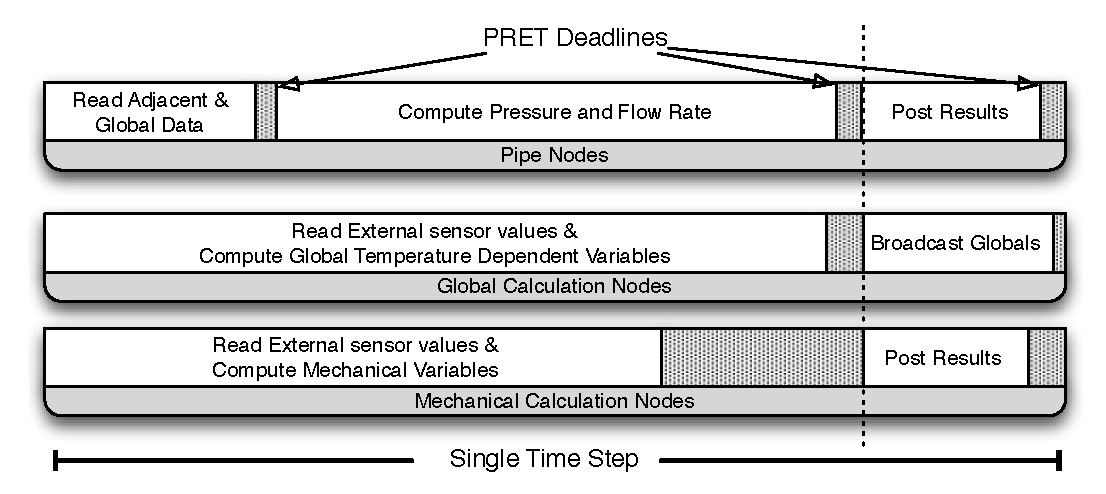
\includegraphics[scale=0.6]{./figs/1dcfd/software_execution_model.pdf}
\caption{Execution of Nodes at Each Time Step}
\label{fig:1dcfd-software_model}
\vspace{-5mm}
\end{figure}

In section~\ref{sec:programming_models} we introduced ISA extensions that provide programmers with explicit timing control in software.  
The implementation of the various timing instructions for PTARM is explained in section~\ref{sec:ptarm_instructions}.
Specifically for this application, we use the specialized timing instruction \emph{delay\_and\_set} as introduced in section~\ref{sec:programming_models}.
The semantics of the \emph{delay\_and\_set} instruction is similar to the deadline instruction introduced by Ip and Edwards\todo{cite}. 
When it is decoded, it first enforces the previously specified timing constraint, then it sets a new timing constraint for the next code block. 
The instruction enforces a minimum execution time within the code, which we use to enforce the synchronized execution of time steps for all nodes.  
Fig.~\ref{fig:1dcfd-software_model} shows the program synchronization points that our timing instruction enforces.
The hatched area in the figure denotes slack time that is generated by the timing instructions.
Each \emph{delay\_and\_set} instruction takes 2 thread cycles because it manipulates a 64-bit value representing time. 
For our computational nodes, 3 timing instructions are used each time step, thus 6 thread cycles of overhead are introduced per time step.
%The overhead is already included in our execution time analysis presented in table~\ref{tab:1dcfd-inst-count}.

The timing instructions provide a very lightweight and simple mechanism to enforce synchronization in software.
No additional run-time system is needed to enforce the execution model, and we avoid the need to use locks or mutex to ensure correct ordering of communicated data. 
%Instead, on a timing predictable architecture, we use time to synchronize the execution all computational nodes.
The same effect can possibly be achieved with no overhead using instruction counting and NOP insertions.
This can certainly be done on any deterministic architecture such as PRET. 
However, NOP insertion is both brittle and tedious. 
Any change in the code would change the timing of the software and insertions need to be adjusted to ensure the correct number of NOPs are added.
Designs now are mostly written in programming languages like the language C and compiled into assembly, making it even more difficult to gauge the number of NOPs needed at design time.
The timing instructions allow for a much more scalable and flexible approach. 
In a system with heterogeneous nodes and different execution times, the timing instructions allow us to set the same timing constraints in all nodes regardless of its execution time.   

The \emph{delay\_and\_set} instruction only enforces minimum execution time, but does not guarantee that the worst-case execution time of all computational nodes meet the timing constraints imposed from the application.
Static timing analysis on all nodes is still required to verify that the worst-case execution time of time steps meets the imposed timing constraints by the application parameters.
However, as soon as the timing constraints are met, there are no additional benefits to improving the execution speed of the computational nodes.
As system time steps are synchronized with sensors that interface with the physical world, and execution is real-time along the engine. 
In this case, precise execution time analysis can help us optimize other system resources, such as power and area, improving the scalability of the approach.
On the other hand, over estimation of execution time could lead to over-provisioning of hardware resources.    
In this application, the computation code on the nodes within each time step contains only a single path of execution, voiding the need for complex software analysis.
Thus, the predictability of the underlying architecture determines how precise the worst-case execution time analysis is.
Communication is handled by the synchronized communication points, which enforces an ordering between the writing and reading of shared data.
This voids the need of any explicit synchronization methods, removing any overhead and unpredictability for communication.
The underlying architecture uses the time-predictable PRET, and implements a latency-deterministic communication network of shared BRAMs on the FPGA. 
These properties allow us to statically obtain an exact execution time for each computation node, which we will show and present in the next section. 

%------------------------------------------------------------------------ 
\subsection {Experimental Results and Discussion}
\label{sec:1dcfd-results}
We use three examples to evaluate our framework.
The first example is a simple waterhammer example taken from Wylie and Streeter~\cite{1978FluidTransients}.
It is similar to the one shown in figure~\ref{fig:1dcfd-DetailedDiagram}, but without the ``T" element and the nodes that branch up.
This example contains an imposed pressure, 5 pipe segments, a valve, and two mechanical input blocks that provide both the reference pressure and the valve angle as a function of time.
We use this simply as a sanity check for the correctness of functionality of our framework.
  
The second and third example cover two common diesel injector configurations: the unit pump and common rail.  
The data for configuring these cases was taken from reference examples provided by Gamma Technologies' GT-SUITE software package~\cite{GTFuel}. 
The unit pump is much like the simple waterhammer case in that there are no branches in the system.  
The input is a defined flow specified by an electronically controlled cam driven pump.  
The output is a single valve.  
There are a total of 73 fluid sub-volumes in this system. 
%
The common rail example is more complex where the topology is roughly that described by the 1D-CFD model in figure~\ref{fig:1dcfd-DetailedDiagram}.  
It has a total of 234 sub-volumes, including 5 ``T" intersections and 4 valves.
Both the GT-SUITE-based models use a 1 $cm$ discretization length, which, using a 1500 $m/s$ wave speed, and a stability factor of 0.8 yields a 5.33\(\mu s\) time step to complete our worst-case instructions for the slowest computational node.

We synthesize all our cores and interconnects on the Xilinx Virtex 6 xc6vlx195t~\cite{v6_manual} with speed grade 3.
Each Virtex-6 FPGA logic slice contains 4 LUTs and 8 flip-flops, and this FPGA contains 31,200 logic slices and 512 18-$KB$ BRAMs.
Each PRET core is clocked at 150 $MHz$ and has 6 threads.
All floating point units are generated from the Xilinx Coregen tool~\cite{xilinx_coregen}, and are configured to maximize DSP slice usage and minimize logic slice usage as much as possible.
We save the logic slices to synthesize as many cores as possible.
Our current PRET implementation, the PTARM, uses an ARM-based ISA, thus our C code is compiled using the GNU ARM cross compiler~\cite{gnu-arm} with the optimization compiler flag set to level 3.  
For these examples, we used a mapping heuristic that grouped nodes requiring same computations onto the same core. 
In the sections below we will show that this heuristic allows us to save hardware resources by synthesizing less floating point units. 

\subsubsection{Timing Requirements Validation}
%\todo{Talk about the shared BRAM makes all communication single cycle.}
In order to ensure that the worst-case computational element can meet the timing requirements, static timing analysis is done on all computational nodes to determine the worst-case execution of each time step.
As discussed in section~\ref{sec:1dcfd-software_architecture}, the computation code within each time step only consists of a single path, simplifying the timing analysis.
The thread-interleaved pipeline provides temporal isolation for all hardware threads, so no timing interference occurs between the threads.
We can safely use the timing analysis done separately for each computational node even as they are executed simultaneously in the architecture.
Because all code, data, and communication channels reside on the BRAMs of the FPGA, the access latency is all deterministically one cycle.
The PTARM architecture provides deterministic execution time for each instruction implemented, and the full list of instruction execution cycles is listed in table~\todo{refer to table in ptarm section}.
Most floating point instructions take only a single thread cycle, as the latency is fully hidden by interleaving the hardware threads in the pipeline.
The more complex floating point square root and divide operations take four thread cycles.
Using the deterministic instruction execution cycles and the compiled code, we are able to obtain the exact thread cycles required for each computational node, which is shown in table~\ref{tab:1dcfd-inst-count}.  

\begin{table}
\begin{center}
\begin{smalltabular}{|l|c|c|c|c|c|c|}
\hline
 & \multicolumn{6}{c|}{Without Interpolation / With Interpolation} \\
\hline
Type	& Mul	& Add/Sub	& Abs	& Sqrt	&Div	&Thread cycles \\ 
\hline \hline
Pipe segment					&10 / 18	&5 / 13		&2 / 2		&0 / 0 		&0 / 0		&51 / 81 \\ 
\hline
Imposed pressure 						&6 / 10		&3 / 7		&1 / 1		&0 / 0 		&0 / 0		&38 / 50 \\ 
\hline
Imposed flow			&5 / 9		&3 / 7		&1 / 1		&0 / 0 		&0 / 0		&40 / 51\\ 
\hline
Valve 						&13 / 17	&5 / 9 		&1 / 1		&1 / 1 		&0 / 0		&55 / 64 \\ 
\hline
Cap 							&4 / 8		&2 / 6 		&1 / 1		&0 / 0 		&0 / 0		&39 / 48 \\ 
\hline
Pipe ``T" 		&16 / 28 	&13 / 25 		&3 / 0		&0 / 0 		&4 / 4		&72 / 111 \\ 
\hline  
\end{smalltabular}
\vspace{-5mm}
\end{center}
\caption{Computational Intensity of Supported Types}
\label{tab:1dcfd-inst-count}
\vspace{-2mm}
\end{table}

%A hardware context switch occurs every processor cycle, and threads are scheduled in a round robin order.
To convert thread cycles to physical time, we use the processor clock speed and number of threads executing in the architecture. 
Given a 150~$MHz$ clock rate and six hardware threads, each thread executes at 25~$Mhz$ in our thread-interleaved pipeline. 
Thus, each thread cycle converted to physical time is 40~$ns$ long.
The unit pump and common rail have a requirement of 5.33~$\mu s$, which gives us 133 thread cycles to complete the computation each time step. 
Table~\ref{tab:1dcfd-inst-count} shows that the ``T'' element, which takes 111 thread cycles with interpolation, is the node with the worst-case execution time, well below the 133 thread cycle constraint. 
For the simple waterhammer example, a bigger discretization $\Delta x$ is used, which leads to a bigger time step than that of the two complex examples.
This validates that we can safely meet the timing requirements, ensuring the correctness of functionality of our implementation.   

\subsubsection{Resource Utilization}

Table~\ref{tab:1cfd-Cores_vs_features} shows the resource usage in logic slices for different configurations of a PTARM core.
Each core uses 7 BRAMs: 3 for the integer unit register set (3 read and 1 write port), 2 for floating point register set (2 read and 1 write port), 1 for the scratchpad, and 1 for the global broadcast receiving memory.
We include the fixed point configuration for reference purposes, as it doesn't contain any floating point units.
The baseline configuration used in our implementation is the ``basic float'', which contains a floating point add/subtracter, a floating point multiplier, and float to fix conversion units.
The ``sqrt'', ``div'' and ``sqrt \& div'' configurations add the corresponding hardware units onto the ``basic float'' configuration. 
Besides the effect of hardware units, we also show the area impact of adjusting the thread count on a single core.

\begin{table}[hbt!]
\begin{center}
\begin{tabular}{|l|c|c|c|c|c|c|}
\hline
Threads per core & 6 & 8 & 9 & 16\\ \hline\hline
Fixed point only  & 572 & 588 & 764 & 779\\ \hline
Basic float  & 820 & 823 & 1000 & 1022 \\ \hline
Float with sqrt  & 987 & 992 & 1146 & 1172 \\  \hline
Float with div  & 1039 & 1051 & 1231 & 1237 \\ \hline
Float with div \& sqrt  & 1237 & 1249 & 1403 & 1413 \\ \hline
\end{tabular}
\vspace{-6mm}
\end{center}
\caption{\small{Number of Occupied Slices per Core on the Virtex 6 (xc6vlx195t) FPGA.}}
\label{tab:1cfd-Cores_vs_features}
\vspace{-2mm}
\end{table}

Two important observations are made from the results of table~\ref{tab:1cfd-Cores_vs_features}.
First, the area increase associated with adding more threads to the core is proportional only to the number of bits required to encode the number of threads.  
For example, running 6 threads or 8 threads (both requiring three bits to encode the thread number) on the processor yields a similar area usage.
But once a 9th thread is introduced, the used area noticeably increases, but remains similar for up to 16 threads. 
This can be explained by understanding the architecture of multi-threaded processors. 
Multi-threaded processors maintain independent register sets and processor states for each thread, while sharing the datapath and ALU units amongst all threads.
The register sets are synthesized onto BRAMs, so the number of bits used to encode thread IDs will determine how big of a BRAM is used for the register set. 
The size of the multiplexers used to select thread states and registers is also determined by the number of bits encoding the thread IDs, not the actual number of threads running. 
Thus, it is possible to increase the number of threads per core with almost negligible impact on area as long as the incremented thread count uses the same number of bits to encode.    
Increasing the thread capacities will allow our architecture to support more nodes in a single FPGA.
However, since hardware threads share the processor pipeline, adding threads slows down the running speed of the individual threads.
Nonetheless, for implementation that have sufficient slack time or require faster performance, adjusting the number of threads could lead to a valuable improvement.
Our precise execution time analysis allows us to determine the maximum number of threads, six in our case, we can support to meet our timing constraints.
An over estimated execution time in this case could lead to under utilizing the hardware by constraining the number of threads to five, resulting in requiring additional cores to implement our 237 node fuel rail example.     

The second observation relates to the resource impact of the floating point square root and divide units. 
Looking at the resource usage for 6 threads on a core, adding a floating point square root unit adds roughly 20.3\% more logic slices than the ``basic float'' configuration.  
Ading a floating point division unit adds roughly 26.7\% more logic slices than the ``basic float" configuration.  
A core with both square root and division unit would use roughly 50.8\% more slices.
These are estimates because the slices occupied might vary slightly based on how the synthesis tool maps LUTs and flip flops to logic slices. 
But they give an intuition to the resource difference used for each configuration.

The actual resource impact can be seen from Table~\ref{table:1dcfd-example_results}, which shows the total slices occupied when the three examples we implemented are synthesized.
In the homogeneous (hom. suffix) configuration, all the cores contain the square root and divide hardware.
In the heterogeneous (het. suffix) configuration, only necessary cores contain square root and divide, the rest use the basic float configuration.  

\begin{table}[htb!]
\vspace{-2mm}
\begin{center}
\begin{smalltabular}{|c|c|c|c|c|c|c|c|}
\hline
\multicolumn{2}{|c}{\multirow{2}{*}{Example}}	& \multicolumn{1}{|@{\hspace{0.5mm}}c@{\hspace{0.5mm}}|}{\multirow{2}{*}{Nodes}}	& \multicolumn{1}{|@{\hspace{0.5mm}}c@{\hspace{0.5mm}}|}{\multirow{2}{*}{Cores / Conn.}}	& \multicolumn{2}{|c|}{Slices / BRAM}  \\
\cline{5-6}
\multicolumn{2}{|c|}{}	&	&	& Absolute	& \multicolumn{1}{|@{\hspace{1mm}}c@{\hspace{1mm}}|}{Relative (\%)}	\\ 
\hline\hline
Water	& het.	& \multirow{2}{*}{12}	& \multirow{2}{*}{2 / 1}	& 1805 / 15	& 5.7 / 2.1 \\ 
\cline{2-2}\cline{5-6}
Hammer	& \multicolumn{1}{|@{\hspace{1mm}}c@{\hspace{1mm}}|}{hom.}	&	&	& 2379 / 15	& 7.6 / 2.1\\ 
\hline
Unit	& het.	& \multirow{2}{*}{73}	& \multirow{2}{*}{13 / 12}	& 10566 / 103	& 33.0 / 15.0\\ 
\cline{2-2}\cline{5-6}
Pump	& hom.	&	&	& 16635 / 103	& 44.0 / 15.0\\ 
\hline
\multicolumn{1}{|@{\hspace{1mm}}c@{\hspace{1mm}}|}{Common}	& het.	& \multirow{2}{*}{234}	& \multirow{2}{*}{39 / 38}	& \multicolumn{1}{|@{\hspace{1mm}}c@{\hspace{1mm}}|}{29134 / 311}	& 93.4 / 45.0 \\ 
\cline{2-2}\cline{5-6}
Rail	& hom.	&	&	& \multicolumn{2}{c|}{N/A} \\ 
\hline
\end{smalltabular}
\vspace{-6mm}
\end{center}
\caption{\small{Total Resource Utilization of Examples Synthesized on the Virtex 6 (xc6vlx195t) FPGA}}
\label{table:1dcfd-example_results}
\vspace{-2mm}
\end{table}

For the simple waterhammer example, since only 2 cores are used, the savings is less noticeable. 
But as the application size scales up, the resource savings of a heterogeneous architecture become more apparent.
The homogeneous approach uses roughly 1.5 times the number of slices our heterogeneous approach uses, which is consistent with the findings in table~\ref{tab:1cfd-Cores_vs_features}.
This proved to be critical for the 234-node common rail example, as only our heterogeneous architecture could implement the design on the xc6vlx195t FPGA while the homogeneous design simply could not fit.
These results also reflect our decision to use a heuristic that groups nodes with the similar computation together. 
By doing so, we can synthesize less hardware floating point units overall, saving hardware resources.
Table~\ref{table:1dcfd-example_results} also shows the BRAM usage for the implemented examples. 
Each interconnect uses 1 BRAM and each core uses 7 BRAMs. 
We see that the BRAM utilization ratio is far below the logic cell utilization, validating our design choice of using BRAMs for interconnects and broadcasts.     

%-------------------------------------------------------------------------
\subsection{Conclusion}
\todo{add more explanation of why this app is impmortant for PRET}
In this application, we presented a novel framework for solving a class of heterogeneous micro-parallel problems.  
Specifically we showed that our approach is sufficient to model a diesel fuel system in real time using the 1D-CFD approach on FPGAs.
To the best of our knowledge, we believe this is the first attempt to attack real-time CFD on this timescale and complexity of problem.
There may exist different implementation options for our application on FPGAs. 
For example, we could attempt the problem in discrete FPGA blocks.  
However, in order to make the application fit in a practical FPGA, we would need to re-use the hardware multipliers, adders, and other functional units.  
This would require a state machine to run it and begins to look a great deal like a processor.

Instead, we use the PRET architecture to ensure timing determinism and implement a light-weight timing based synchronization on a multicore PRET architecture.
We set up a configurable heterogeneous architecture that leverages the programmability of FPGAs to efficiently synthesize the design for efficient area usage. 
Our results show ample resource savings, proving that our approach is practical and scalable to larger and more complex systems.

%	It is important to understand that in our framework, 
	%PRET timing instructions are used to enforce the periodic behavior of the application, while the precise timing analysis allows us to ensure that the timing requirements are met. 
	%Communication and synchronization of the cores are timing based, thus adding cores or threads does not add any overhead or affect performance.

%We plan to continue to extend this work along several lines.  
%From the application perspective, we continue to add more flow element types to our library and compare our results to more complex flow systems.  
%We also plan to examine more closely the integration of mechanical and electrical nodes in our library.
%For the hardware architecture, we can to explore multi-rate timing of nodes to allow for differences in electrical, fluid, and mechanical timesteps.  
%

\section{Eliminating Timing Side-Channel-Attacks}
\label{sec:app_side_channel_attack}

Encryption algorithms are based on strong mathematical properties to prevent attackers from deciphering the encrypted content. 
%only timing attacks
However, their implementations in software naturally introduce varying run times because of data-dependent control flow paths.
Timing attacks~\cite{Kocher96timingattacks} exploit this variability in cryptosystems and extract additional information  from executions of the cipher.
These can lead to deciphering the secret key.
Kocher describes a timing attack as a basic signal detection problem~\cite{Kocher96timingattacks}. 
The ``signal'' is the timing variation caused by the key's bits when running the cipher, while ``noise'' is the measurement inaccuracy and timing variations from other factors such as architecture unpredictability and multitasking. 
This signal to noise ratio determines the number of samples required for the attack -- the greater the ``noise,'' the more difficult the attack. 
It was generally conceived that this ``noise'' effectively masked the ``signal,'' thereby shielding encryption systems from timing attacks. 
However, practical implementations of the attack have since been presented~\cite{remoteattackspracticle,DKLMQW98,SCAsurvey} that clearly indicate the ``noise'' by itself is insufficient protection. 
In fact, the architectural unpredictability that was initially believed to prevent timing attacks was discovered to enable even more attacks.
Computer architects use caches, branch predictors and complex pipelines to improve the average-case performance while keeping these optimizations invisible to the programmer.
These enhancements, however, result in unpredictable and uncontrollable timing behaviors, which  were all shown to be vulnerabilities that led to side-channel attacks~\cite{2004-bernstein-cachetiming,Percival05cachemissing,Onur07predictingsecret,2009-x86timing}.

In order to not be confused with Kocher's~\cite{Kocher96timingattacks} terminology of \textit{timing attacks} on algorithmic timing differences, we classify all above attacks that exploit the timing variability of software implementation \textit{or} hardware architectures as \textit{time-exploiting attacks}. 
In our case, a \textit{timing attack} is only one possible \textit{time-exploiting attack}.
Other time-exploiting attacks include branch predictor, and cache attacks.
Examples of other side-channel attacks are power attacks~\cite{Messerges99investigationsof,Kocher99differentialpower}, fault injection attacks~\cite{biham97differential,Feng_efficientcomb}, and many others~\cite{SCAsurvey}.
%Bernstein at al.\cite{2004-bernstein-cachetiming} introduced the vulnerabilities of caches to side channel attacks; Aciicmez at al.\cite{Onur07predictingsecret} showed us how the branch predictor could be used as a side channel; 

%Attackers take advantage of different properties of the implementation such as run time, power usage, and even the behavior after manually injecting faults into the system's operation. 

In recent years, we have seen a tremendous effort to discover and counteract side-channel attacks on encryption systems~\cite{biham97differential,2009-x86timing,99designprinciples,fbscc,branchpredict,Kelsey98sidechannel,blindingrsa,cachepartition,sidechannelprocarch}.
However, it is difficult to be fully assured that all possible vulnerabilities  have been discovered.
The plethora of research on side-channel exploits~\cite{2009-x86timing,biham97differential,99designprinciples,fbscc,branchpredict,Kelsey98sidechannel,blindingrsa,cachepartition,sidechannelprocarch} indicates that we do not have the complete set of solutions as more and more vulnerabilities are still being discovered and exploited.
Just recently, Coppens et al.~\cite{2009-x86timing} discovered two previously unknown time-exploiting attacks on modern x86 processors caused by the out-of-order execution and the variable latency instructions.
This suggests that while current prevention methods are effective at \textit{defending} against their particular attacks, they do not \textit{prevent} other attacks from occurring.
This, we believe, is because they do not address the root cause of time-exploiting attacks, which is that run time variability \textit{cannot be controlled} by the programmer.

It is important to understand that the main reason for time-exploiting attacks is \textit{not} that the program runs in a varying amount of time, but that this variability \textit{cannot be controlled} by the programmer. 
The subtle difference is that if timing variability is introduced in a controlled manner, then it is still possible to control the timing information that is leaked during execution, which can be effective against time-exploiting attacks. 
However, because of the programmer's \textit{lack of control} over these timing information leaks in modern architectures, noise injection techniques are widely adopted in attempt to make the attack infeasible.
These include adding random delays~\cite{Kocher96timingattacks} or blinding signatures~\cite{Kocher96timingattacks,blindingrsa}. 
Other techniques such as branch equalization~\cite{Molnar05theprogram,SCAsurvey} use software techniques to rewrite algorithms such that they take equal time to execute during each conditional branch. 
We take a different approach, and  directly address the crux of the problem, which is the \textit{lack of control} over timing behaviors in software. 
%Computer architects have introduced caches and complex pipelines to improve the average-case performance while keeping these optimizations invisible to the programmer. 
%However, these improvements often attribute to the unpredictable and uncontrollable timing behaviors, which result in time-exploiting attacks.
We propose the use of an embedded computer architecture that is designed to allow predictable and controllable timing behaviors.

%By proposing a predictable architecture, it may seem that we are making the attacker's job easier by reducing the ``noise'' 
At first it may seem that a predictable architecture makes the attacker's task simpler, because it reduces the amount of ``noise'' emitted from the underlying architecture.
However, we contend that in order for timing behaviors to be controllable, the underlying architecture \textit{must} be predictable.
This is because it is meaningless to specify any timing semantics in software if the underlying architecture is unable to honor them.
And in order to guarantee the execution of the timing specifications, the architecture must be predictable. 
%Hiren - I removed this because it was said at the very end of the introduction
%we argue that a combination of software techniques to control execution times, and hardware techniques that make an architecture predictable are necessary to thwart time-exploiting attacks.
%\textcolor{red}{\FIXME{Sounds too casual -- rephrase}Let us also not forget that the architecture unpredictability which was once thought to shield systems from timing attacks were eventually discovered to be the main vulnerabilities in other side-channel attacks, mainly because they were uncontrollable.}
Our approach does not attempt to increase the difficulty in performing time-exploiting attacks, but to eliminate them completely. 
%As such, we argue that only by providing a timing predictable architecture, can we allow controllable timing behaviors, which removes the source of time-exploiting attacks. 

For this application, we present PRET in the context of embedded cryptosystems, and show that an architecture designed for predictability and controllability effectively eliminates all time-exploiting attacks.
%The PREcision Timed architecture~\cite{pret_cases08} (PRET) allows for precision timing control, and was originally proposed for real-time embedded systems.
%Originally proposed by Lickly et al~\cite{pret_cases08}, PRET provides instruction-set architecture (ISA) extensions that allow programmers to control an algorithm's temporal properties at the software level.
%To guarantee that the timing specifications are honored, PRET provides a predictable architecture that replaces complex pipelines and speculation units with multithread-interleaved pipelines, and replaces caches with software-managed fast access memories.  
%This allows PRET to maintain predictability without sacrificing performance.
We target embedded applications such as smartcard readers~\cite{99designprinciples}, key-card gates~\cite{rfidcrypto}, set-top boxes~\cite{99designprinciples}, and thumbpods~\cite{schaumont2003tts}, which are a good fit for PRET's embedded nature.
We demonstrate the effectiveness of our approach by running both the RSA and DSA~\cite{dss} encryption algorithms on PRET, and show its immunity against time-exploiting attacks.
%The combination of ISA extensions and architectural design decision ensures that PRET can provide controllable timing semantics in software, which eliminate the vulnerability of time-exploiting attacks. 
%This makes it an appropriate match for cryptosystems.
This work shows that a disciplined defense against time-exploiting attacks requires a combination of software and hardware techniques that ensure controllability and predictability.

\subsection{Background}
% 1 - 1.5 page
Kocher outlined a notion of timing attacks~\cite{Kocher96timingattacks} on encryption algorithms such as RSA and DSS that require a large number of plaintext-ciphertext pairs and a detailed knowledge of the target implementation.  
By simulating the target system with predicted keys, and measuring the run time to perform the private key operations, the actual key could be derived one bit at a time.
Kocher also introduced power attacks~\cite{Messerges99investigationsof,Kocher99differentialpower}, which use the varying power consumption of the processor to infer the activity of the encryption software over time. 
These played a large role in stimulating research in side-channel cryptanalysis~\cite{mmthesis,Kelsey98sidechannel}, which also found side-channel attacks against IDEA, RC5 and blowfish~\cite{Kelsey98sidechannel}. 
Fault-based attacks~\cite{biham97differential,fbscc,Feng_efficientcomb} were introduced by Bihan et al.~\cite{biham97differential}.
These attacks attempt to extract keys by observing the system behavior to generated faults.
For the side-channel attacks that we have missed, Zhou~\cite{SCAsurvey} presents a survey on a wide range of side-channel attacks.

Dhem et al.~\cite{DKLMQW98} demonstrated a practical implementation of timing attacks on RSA for smart cards and the ability to obtain a 512-bit key in a reasonable amount of time.
Several software solutions such as RSA blinding~\cite{Kocher96timingattacks,blindingrsa}, execution time padding~\cite{Kocher96timingattacks}, and adding random delays~\cite{Kocher96timingattacks} have been proposed as possible defenses against this attack. 
However, these solutions were not widely adopted by the general public until Brumley et al.~\cite{remoteattackspracticle} orchestrated a successful timing attack over the local network on an OpenSSL-based web server.
This motivated further research on timing attacks for other encryption algorithms such as ECC~\cite{Feng_efficientcomb} and AES~\cite{2004-bernstein-cachetiming}.
In particular, Bernstien's attack on AES~\cite{2004-bernstein-cachetiming} targeted the the run time variance of caches.
The introduction of simultaneous multi-threading (SMT) architectures escalated this type of attack on shared hardware components. 
Percival~\cite{Percival05cachemissing} showed a different caching attack method on SMT, made possible because caches were shared by all processes running on the hardware architecture. 
Ac�i�mez et al. introduced branch predictor
attacks~\cite{Onur07predictingsecret,branchpredict} that monitor control flow by
occupying a shared branched predictor. Compiler and source-to-source transformation techniques~\cite{2009-x86timing,Molnar05theprogram} have also been developed to thwart side-channel attacks.

Wang et al.~\cite{sidechannelprocarch} identified the causes of the timing attacks to be the underlying hardware. 
In particular, their work focuses on specialized cache designs, such as Partition-Locked Caches~\cite{cachepartition} and Random Permutation caches~\cite{sidechannelprocarch} that defend against caching attacks in hardware.
Very recently, Coppens~\cite{2009-x86timing} discovered two previously unknown attacks on the complex pipeline run time variance of x86 architectures.

Our work builds upon the experiences of these.
Most solutions employ either exclusively hardware or software techniques to defend against attacks.
We recognize that a complete solution to control temporal semantics requires a combination of both software and hardware approaches to defend against and prevent future side-channel attacks.
Hence, we present an effort that includes timing control instructions to control execution times in software, and a predictable processor architecture to realize the instructions. 
By doing this, we completely eliminate the source of leaked information used by time-exploiting attacks, rendering the system immune against such attacks.
%We now explain in more detail the architecture of PRET in the context of cryptosystems.

%The architectural design of PRET is to allow: 1) better meaning of deadline instructions, 2) you need predictable underlying hardware, 3) which means timing behaviors of threads must be decoupled. 

% PRET is designed to provide controllable timing behaviors.
% This properties has proved to be of critical importance to real-time systems~\cite{pret_cases08}, and time-exploiting attacks have shown that they are just as critical for security systems.
% We present the PRET architecture in detail in the context of time-exploiting attacks.
%This is because PRET eliminates the source of time exploiting attacks, which is the unpredictability and uncontrollability prevalent in modern computer architectures.

%% \begin{figure}
%%   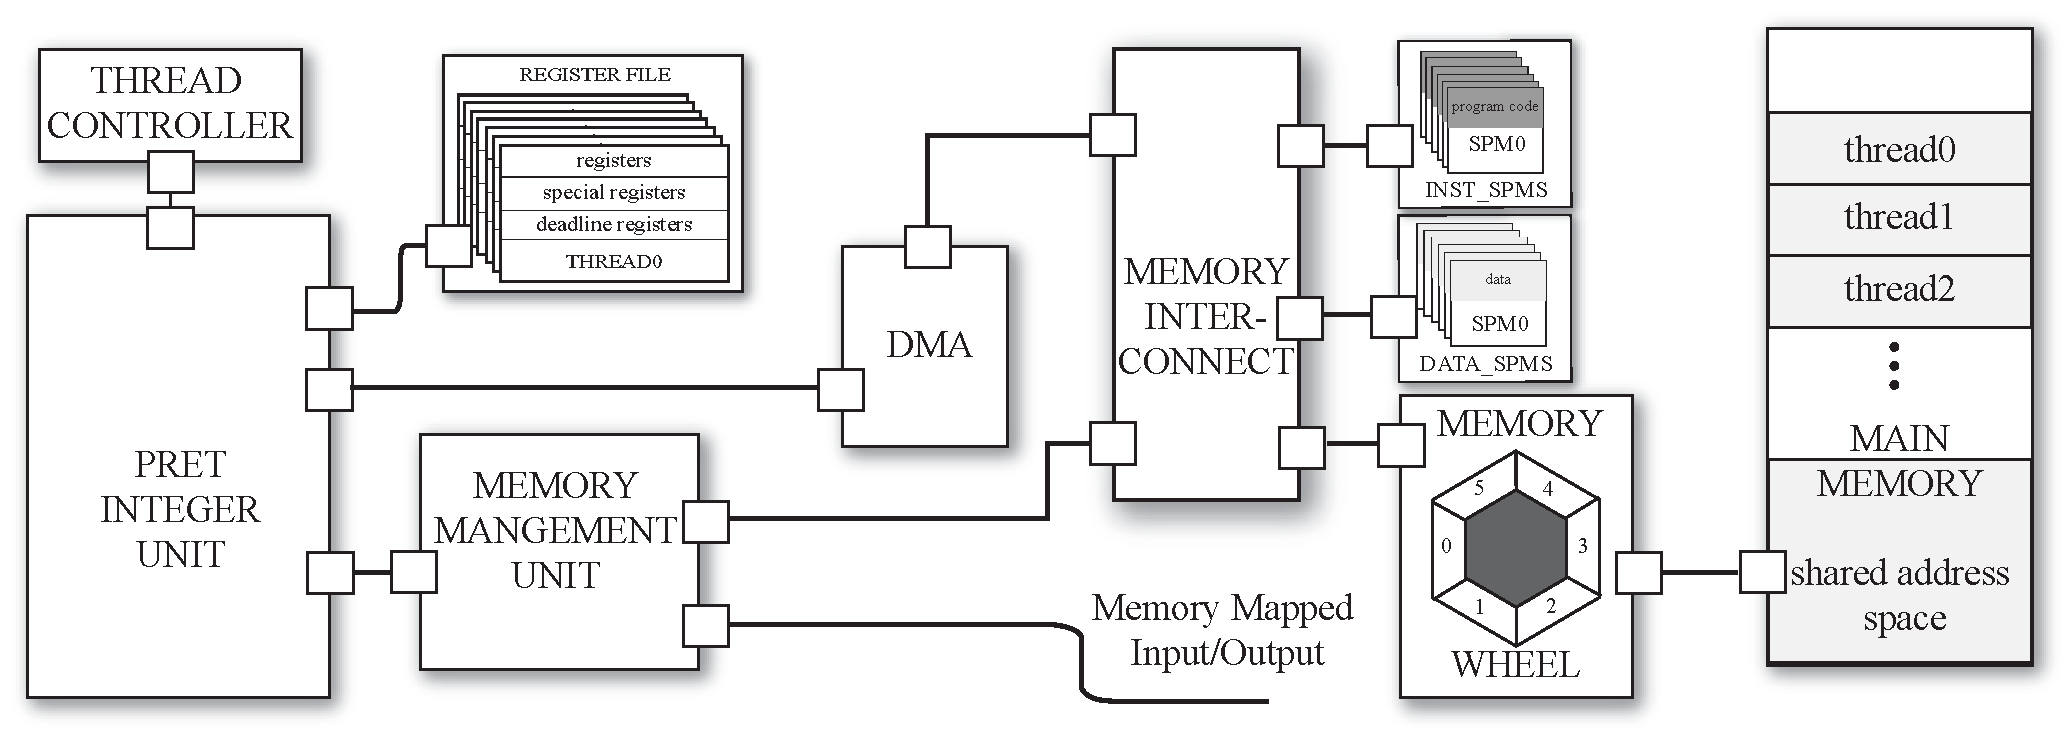
\includegraphics[width=\textwidth]{./images/top_arch.pdf}
%%   \caption{Unit Diagram for PRET Architecture. Reproduced with permission~\cite{pret_cases08}. }
%%   \label{fig:compview}
%%   \end{figure}

\subsection{A Precision Timed Architecture for Embedded Security}
The foundation of time-exploiting attacks exploits the uncontrollable timing variability introduced to programs by underlying the implementation of encryption algorithms.
Software implementations naturally introduce varying run times because of data-dependent control flow paths.
Modern computer architectures create unpredictable execution times by abstracting away hardware optimizations meant to improve average case performance.      
In this section we will present several features of PRET that bring \textit{controllability} over timing to software, eliminating the origin of the attacks.
We will discuss the software extensions that allow timing specification in programs, and the predictable architecture to comply with these specifications.
These two approaches cannot be separated.
A predictable architecture by itself would only ease the feasibility of an attack, and software timing specifications are meaningless if they cannot be met by the hardware. 
By combining both hardware and software solutions, we yield a timing predictable and controllable architecture. 
Thus, by design, PRET prevents leakage of any timing side-channel information, and eliminates the core vulnerability of time-exploiting attacks.

\subsubsection{Controlling Execution Time in Software}
It is extremely difficult to control and reason about timing behaviors in software, even with adequate understanding of the underlying architecture.
Current instruction-set architectures (ISA) have neglected to bring the temporal semantics of the underlying architecture up to the software level.
Thus, architecture designs have introduced clever techniques to improve on average case execution time of the instructions, at the expense of introducing variability in instruction execution time.
These architecture improvements are hidden to the software behind the abstraction of the ISA.   
%The difference in execution time for different paths of the program are often a result of optimizations to the program performance.
This proves to be costly in terms of security, because it uncontrollably leaks timing information which can correlate to the secret key.

In section~\ref{sec:programming_models} we introduced several ISA extensions that add time controlling behaviors to software. 
The extensions provide timing instructions that enable a programmer to have more control of execution time in software.
These instructions do not physically alter processor speed, or modify the execution time of instructions on the architecture.
Instead, they are meant to aid the programmer in dealing with timing variability from data-dependent control flow paths by allowing the programmer to interact with various execution time behaviors in software. 
This includes the ability to specify a desired execution time for code segments, and the ability to detect and handle situations when the execution time exceeds the desired amount.
Specifically in this context, the ability to enforce a minimum execution time for code segments proves extremely useful for mitigating the varying execution speeds exhibited by algorithms or code segments.  
We showed in section~\ref{sec:1dCFD} how the \emph{delay\_and\_set} instruction can be used to synchronize execution and communication of different nodes for an implementation of a real-time 1D-CFD simulation.  
Encryption algorithms can exhibit varying execution time behaviors depending on the bits of the encryption key.
The algorithm follows different execution paths if a particular bit in the key is set or not, allowing attackers to exploit this execution time variance to obtain the key.
By using the timing instructions provided by the PRET architecture, we can mitigate the effects of this, eliminating the exploit causing this timing  attack.  

At the expense of more programming effort, other solutions have been proposed to alter and pad the execution time of different execution paths~\cite{Kocher96timingattacks} to shield against the timing variability of the algorithm. 
At a glance it might seem that the timing instruction are a similar solution to these proposals, however, the principles are inherently different. 
While effective against certain time-exploiting attacks, existing solutions alter the underlying algorithm implementation in attempt to manually pad or distort the execution time. 
These solutions are not only algorithmically specific, but could lead to unnecessarily degrading of the performance of encryption algorithms. 
The timing instructions, on the other hand, allows for a separation of concern between the functionality and timing behavior of the code. 
The programmer can implement the correct functionality of the algorithm, then use timing instructions to regulate its timing behavior.
The subtle difference will be more apparent in section~\ref{sec:rtencrypt-results} when we show two different implementations of the RSA encryption that both use timing instructions to regulate execution time.
One implementation mimics existing execution time padding solutions, and the second implementation uses timing instructions to enforce an overall execution time of the RSA algorithm. 
We present performance comparisons and show that explicit timing control instructions could prove more beneficial than simple execution time padding.  

 %in the results section in section~\ref{sec:rtencrypt-results}. 
% The first implementation mimics the behavior of an existing execution time padding solution by forcing the execution time of all modular exponent operations, regardless of the bit value from the encryption key. 
% This solution leads the execution down the worst-case execution path for any encryption key, which we argue is unnecessarily degrading the algorithm performance.     
% Our second implementation uses statistical analysis on the run time of various input keys in encryption algorithms to determine the enforced execution time of the algorithm. 
% This leads to a modest performance improvement compared to the first approach, as the execution path is not forced down the worst-case path.

%We observe the normal distribution of execution times for the RSA encryption, and chose an execution time that covered roughly 97\% of the keys running in the RSA algorithm.    
%Without modifying the algorithm itself, the timing instructions regulated the execution time to   

%However, because these don't change architectural behavior, 
The timing instructions provide a method to control the timing behavior of a program in software.
However, they do not change the behavior of the underlying architecture.
If the underlying architecture makes the reasoning of execution time difficult, then these instructions become more difficult to use.
Timing instructions alone do not prevent attacks that exploit architectural designs to inject execution time variances~\cite{Percival05cachemissing,branchpredict} and obtain side-channel information. 
We argue that a \textit{predictable} architecture is also required to eliminate timing exploiting attacks.

\subsubsection{Predictable Architecture}
\paragraph {Pipeline}
In order to improve instruction throughput and performance, modern processor architectures implement pipelines to execute multiple instructions in parallel.
This requires handling of pipeline hazards, which are caused by dependencies in instruction sequences. 
Conditional branches are the perfect example -- the pipeline cannot fetch and begin executing the next instruction without knowing which instruction to fetch. 
Since a conditional branch usually takes more than one cycle to resolve, the processor is forced to stall until the branch is resolved. 

Computer architects use clever speculative techniques to mitigate the effects of pipeline hazards and to substantially improve the average-case performance.
For example, branch predictors are used to guess the next instruction needed by the processor for branches~\cite{Grunwald98confidenceestimation}.
This allows the processor to execute instructions speculatively while rolling back only when needed. 
%If the speculation is correct, there is no performance penalty, otherwise, the pipeline is flushed and a new instruction stream is fetched.
While these speculative techniques improve the average-case performance, they introduce several side effects. 
%they result in computer architectures that are \textit{unpredictable}, and \textit{uncontrollable}. 
% \FIXME{Isaac: I find that it would be better to say that these architectures are unpredictable, which make cycle-counting and static prediction of execution times virtually impossible. The uncontrollability has two issues: 1) it's not possible to determine the execution times due to unpredictability, and 2) no method of allowing to do so either (no instructions)}
First, they create \textit{timing variations}.  
Depending on the outcome of its speculation, the processor might need to discard the wrongly speculated work, and re-execute the correct instructions. 
Second, these units are \textit{unpredictable}.
Since these units are shared by all software processes concurrently running on the processor, the states of speculation units are heavily dependent on the different interleaving of processes. 
This means that a process can unknowingly be affected by other processes, since the speculation state is shared between them~\cite{leethreads}.
Because the goal of these speculation techniques is to improve program performance without effort from the programmer, the controls of these speculation units are concealed from the programmer, and cannot be directly accessed in software. 
Thus, these side effects result in \textit{uncontrollable} timing behaviors in the program.

Several Multithreaded architectures enable more opportunities to exploit the uncontrollable timing behaviors.   
Multithreading utilizes thread-level parallelism by introducing multiple hardware threads in the processor.
This allows the execution of another hardware thread during pipeline stalls like branches or memory accesses.
However, typical multithreaded architectures share hardware units effecting execution time between hardware threads, enabling threads to covertly affect other threads execution time.  
The class of Simultaneous Multithreading (SMT) architectures presents an example of this.
Here, the hardware threads share multiple execution units and execute in parallel depending on a hardware scheduler. 
Attackers exploit such designs by running a spy thread that executes concurrently with a thread that implements the encryption algorithm.
This spy thread probes the components shared with the encryption thread~\cite{Percival05cachemissing,branchpredict} by forcefully occupying the shared units and observing when they are evicted by the encryption thread. 
The announcement of this vulnerability caused Hyper-Threading, Intel's implementation of SMT, to be disabled by default in some Linux distributions because of its security risks~\cite{hyperthreadharmfulsite}.
For general purpose applications, these side effects pose insignificant threats, but for security applications, the consequences are uncontrollable sources of side-channel information leakages.

The PREcision Timed (PRET) architecture is a timing predictable architecture  proposed for real-time embedded systems.
As discussed in chapter~\ref{section:pret_thread_pipeline}, PRET employs a thread-interleaved pipeline, a multithreaded pipeline that employs a predictable round-robin thread scheduling policy between the hardware threads every cycle.
Instructions from each thread are predictably fetched into the pipeline every $n$ cycles, where $n$ is the number of hardware threads. 
If $n$ is greater than the number of stall cycles needed for data dependency hazards, then we effectively remove those hazards because the data value is available during the next cycle in which the thread is dispatched. 
For example, if we set $n$ to be the number of stages in the pipeline, then we eliminate the need for any data forwarding/bypassing logic, along with the need for hardware speculation units such as branch predictors.
Most importantly, the hardware threads are temporally isolated, meaning that no threads can affect each others timing behavior.  
Each individual hardware thread maintains their own copy of the processor state (program counter, general purpose registers, stack pointer, etc.), and each hardware thread runs independently with no shared state in the pipeline. 
Because of the simple and transparent thread-scheduling policy, each hardware thread gets dispatched in a predictable way that cannot be affected by other hardware threads. 
Thread-interleaved pipelines allow us to gain higher instruction throughput without the harmful side effects.

\paragraph{Memory System}
The memory system presents another opportunity for attackers to gain side-channel information.
The high clock speed of modern processors combined with the high latency to access main memory results in sometimes hundreds of cycles stalled when the processor needs to access the main memory.
On-chip fast access memories are used to bridge this access latency, creating a \emph{memory hierarchy}.
Caches are \textit{hardware-controlled} fast-access memories that predict and prefetch data from main memory based on temporal and spatial locality of data accesses from the processor.
If the cache control speculation is accurate, then access to data can complete in one cycle, and no stall in the pipeline is required.
However, when a misprediction occurs, data needs to be fetched from the main memory, causing a drastic difference in the access time~\cite{thiele:04:predictable}.
Caches abstract away this memory hierarchy and access latency variation from the programmer by managing the cache contents in the hardware.  
Because threads and processes share the same memory system, attackers can probe the memory access patterns of the encryption process by evicting shared cache lines and observing the timing variation it causes~\cite{Percival05cachemissing}.
This is possible because the memory hierarchy is abstracted away from the programmer, resulting in \emph{uncontrollable} timing behaviors. 
%The cache states are manged in hardware, and shared by all threads and processes.   

PRET utilizes scratchpads memories (SPM) instead of caches in its memory hierarchy.  
SPMs are fast access memories controlled by software. 
SPMs use less power and occupy less area~\cite{Banakar2002} because no speculation logic is needed. 
SPMs occupy a distinct address space, which exposes the memory hierarchy to the programmer, instead of abstracting it away like caches.  
The allocation of data between memory and SPM is done with explicit instructions, either at compile time by the compiler or manually by the programmer.
This gives the software control over memory access latencies, and provides a predictable execution time of the program.
The performance of SPMs vary based on the data access patterns of the application, but since the control is in software, it is possible to tune the allocation scheme to achieve even better performance than a generic cache for specific applications. 
There are abundant ongoing research on allocation schemes and methods for optimizing the performance of SPMs~\cite{avissar2002oma,Bandyopadhyay:EECS-2006-105,Patel:EECS-2008-115,WCETSPM,compilerSPM}. 
SPMs can be found in the Cell processor~\cite{cellproc}, which is used in Sony PlayStation 3 consoles, and NVIDIA's 8800 GPU, which provide 16KB of SPM per thread-bundle~\cite{8800gpu}.
Although this comes at the cost of more programing effort, but it is not uncommon to see platform specific tuning of software for performance purposes. 
For example, high performance parallel algorithms are often fine tuned to work on block sizes depending on the cache size and replacement policy of the platform, and re-tuned when running on different platform.

For security purposes, the scratchpad on PRET is configured to provide each hardware-thread a private scratchpad region so the scratchpad contents cannot be modified or monitored by spy threads on running another hardware thread.    
This prevents shared resource time-exploiting attacks on the fast access memory across hardware threads.
Even if an encryption process is sharing a hardware thread with another process, the contents of the scratchpad is controlled in software or statically compiled in by the compiler.
The thread managing supervisor code can manage the contents on the scratchpad before the processes are scheduled and unscheduled, preventing a spy process from affecting the execution time of the encryption process. 
Clearly, the edge that SPMs give over conventional caches is their \emph{controllability} in software, thus preventing unwanted timing side-effects from attackers and spy threads, even though the SPM is shared by software processes.
%If caches must be used, hardware additions to the cache
%Partition locked caches, which allows software processes to to lock cache lines which have proven successful against cache attacks~\cite{cachepartition}, can be implemented. 

Although no known attacks have exploited main memory access, typical DRAM controllers also result in variable memory access latencies, and are shared amongst all threads and processes within the system. 
A predictable DRAM controller is designed and interfaced with the thread-interleaved pipeline of PRET to provide predictable memory access latencies to all threads. 
The DRAM controller privatizes DRAM bank resources to remove bank conflicts and fully utilize bank level parallelism on the DRAM.  
Each hardware thread in the thread-interleaved pipeline is mapped to a privatized DRAM bank resource.
On the backend, the bank resources are accessed in a round robin order fashion, to remove temporal interference between accesses to the bank resources.
All memory accesses from the hardware threads are isolated from each other, removing any possibilities of cross-thread side-channel attacks from the shared memory controller.
The DRAM memory access latencies are decoupled from the data access patterns, thus, even processes on the same hardware thread that access the same bank resources cannot alter each others execution time in attempt to gain side-channel information.  
More details on the PRET DRAM controller is presented in section~\ref{sec:pret_dram_controller}.

We acknowledge the many efforts to counteract timing attacks with algorithm rewrites to control and balance the run time of the algorithm. 
These efforts while successful, are ad-hoc, counteracting specific attacks without prevention of others.
Without tackling the origin of time-exploiting attacks, we believe that more exploits will eventually be discovered, attacking the \emph{uncontrollable} execution time variation caused by the shared resources of hardware or software control flow.  
The PRET architecture is designed to ensure repeatable and predictable timing behavior of programs by providing control of timing properties in software and a predictable architecture that provides temporal isolation for hardware threads and processes.
PRET is impenetrable known attacks such as branch predictor attacks~\cite{Onur07predictingsecret}, cache attacks~\cite{Percival05cachemissing} or other attacks on the pipeline~\cite{2009-x86timing}.
The more importantly, the predictable architecture design removes the root cause of time-exploiting attacks -- the \emph{uncontrollable} timing variations caused by unpredictable hardware components or software control flows.     

\subsection{Case Studies}
\label{sec:rtencrypt-results}
In the following section we will show results of two encryption algorithms running on PRET. 
All experiments are run on the cycle accurate simulator of the PRET architecture described in~\cite{pret_cases08}.
The simulator implements the SPARC v8 instruction set, and employs six threads on a six stage thread-interleaved pipeline.
Programs are written in C and compiled using a standard gcc cross compiler from Gaisler research labs~\cite{GAISLER}.
This PRET implementation implements a simple processor extension inspired by Ip and Edwards~\cite{ip2006processor} that adds timing instructions to the ISA.
To be consistent with the terminology used in~\cite{ip2006processor}, we call this instruction the \textit{deadline instruction}.
This deadline instruction has similar semantics to the \emph{delay\_and\_set} instruction introduced in section~\ref{sec:programming_models}. 
It first ensures the previous deadline specified is met, then sets the deadline for the next instruction sequence.
The deadline instruction specifies time in units of thread cycle, which is a thread's perceived cycle.
  
% The deadline instruction is used to load values into a special set of registers, called the \textit{deadline registers}. 
% In ~\cite{ip2006processor}, these registers are decremented each clock cycle in hardware, and act as hardware cycle counters. 
% Whenever the processor executes a deadline instruction, it first checks the corresponding deadline register's contents. 
% If it is zero, then the value specified in the instruction is loaded into the register, and the program continues. 
% If not, the processor replays this instruction until the value reaches zero. 
% Figure ~\ref{fig:timing_want} shows a simple illustration of what the deadline instructions look like.
% By enclosing instruction blocks within two deadline instructions, we can specify that the enclosing code block should run for x or y cycles.
% In ~\cite{ip2006processor}, this instruction was implemented for a single cycle processor. 
% PRET extended this instruction to be used in a multi-threaded pipeline architecture. 
% We will later show a more concrete example of how this instruction is extended for PRET.

% \begin{wrapfigure}[13]{l}{.4\textwidth}
%   \centering
%   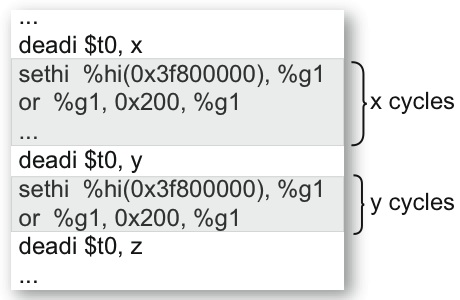
\includegraphics[scale=.7]{./figs/RTencrypt/timing_want.jpg}
%   \caption{A method to express timing requirement in software.}
%   \label{fig:timing_want}
% \end{wrapfigure}

%%Talk about the different in decrementing deadlines in PRET vs
%%original paper?
%This instruction allows a user to specify the execution time of the code enclosed within the deadline instructions. 


% \subsubsection{Timing instructions on PRET}
% 
% \begin{wrapfigure}[11]{r}{.4\textwidth}
% %\begin{SCfigure}
%   \centering
%   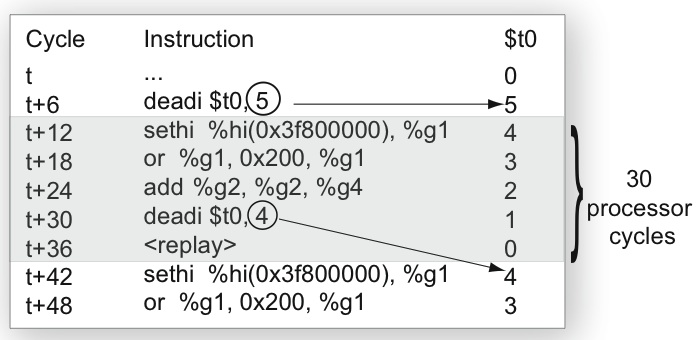
\includegraphics[scale=.53]{./figs/RTencrypt/timing_instructions.jpg}
%   \caption{A simple example using deadline instructions on PRET}
%   \label{fig:deadline}
% %\end{SCfigure}
% \end{wrapfigure}
% 
% Since PRET has multiple hardware threads, each hardware thread contains its own set of deadline registers, which are decremented every time an instruction from that thread is fetched into the pipeline.
% Specifically, PRET has six hardware threads, so each hardware thread's deadline registers are decremented every six processor cycles.
% Figure~\ref{fig:deadline} shows a concrete example of the execution of one thread on PRET using the deadline instruction.
% The three instructions enclosed between the deadline instructions take exactly 30 cycles to execute. 
% \textit{\$t0} shows the contents of deadline register 0. 
% The processor cycle is shown to the left of the instruction.
% When the first deadline instruction is executed, the instruction will simply load 5 into deadline register 0 and continue because the value of \emph{\$t0} is currently 0.
%  When the second deadline instruction is executed, since the value of \emph{\$t0} is not decremented to zero yet, this instruction will be replayed. 
% Only at \emph{t+36} cycles will the value 4 be loaded into deadline register 0.
% This ensures that the code enclosed will take 30 cycles to execute, as specified in the first deadline instruction. 
% We will show two real-world examples of using deadline instructions with encryption algorithms later in the case study section.

\subsubsection{RSA Vulnerability}

The central computation of the RSA algorithm is based primarily on modular exponentiation. 
This is shown in algorithm~\ref{alg:rsa}.
Of the inputs, $M$ is the message, $N$ is a publicly known modulus, and $d$ is the secret key.  
Depending on the value of each bit of $d$ on line 4, the operation on line 5 is either executed or not. 
This creates variation in the algorithm's execution time that is dependent on the key, as mentioned in \cite{Kocher96timingattacks}.

\begin{minipage}[h]{0.4\textwidth}
  \scriptsize
\begin{algorithm}[H]
\label{alg:rsa}
  \LinesNumbered
  \SetAlgoVlined
\KwIn{M, N, d = $(d_{n-1}d_{n-2} . . . d_{1}d_{0})$}
\KwOut{S = M$^{d}$ mod N}
S $\leftarrow$ 1 \\
\For{j = n - 1 $. . .$ 0} {
S $\leftarrow$ S$^{2}$ mod N \\
\If{d$_{j}$ = 1} {
S $\leftarrow$ S $\cdot$ M mod N
}
\textbf{return} S
}
\caption{RSA Cipher}
\end{algorithm}
\end{minipage}
\begin{minipage}[h]{0.6\textwidth}
  \scriptsize
\begin{algorithm}[H]
  \LinesNumbered
  \SetAlgoVlined
\KwIn{M, N, d = $(d_{n-1}d_{n-2} . . . d_{1}d_{0})$}
\KwOut{S = M$^{d}$ mod N}
S $\leftarrow$ 1 \\
\For{j = n - 1 $. . .$ 0} {
/* 110000 is 660000$\div$6 cycles, since deadline registers are decremented every 6 cycles.*/ \\
\textbf{dead(110000);}\\
 S $\leftarrow$ S$^{2}$ mod N \\
\If{d$_{j}$ = 1} {
S $\leftarrow$ S $\cdot$ M mod N
}
\textbf{dead(0)}; \\
\textbf{return} S
}
\caption{RSA Cipher with deadline instructions}
\label{alg:rsa_w_dead}
\end{algorithm}
\vspace{2mm}
\end{minipage}


%Our analysis of the algorithm demonstrated that a significant portion of the variation in the algorithm's execution time could be attributed to the branch in the loop above.  
When the reference implementation of RSA (RSAREF 2.0) was ported to the PRET architecture, single iterations of the loop varied in execution time almost exclusively due to the value of d$_{j}$, which is the j$^{th}$ bit of the key. 
The triangle points in figure \ref{fig:modexp} show the measured run time of each iteration in the for loop (lines 2--6) in algorithm \ref{alg:rsa}. 
Each iteration took approximately either 440 or 660 kilocycles, with very little deviation from the two means.
As a simple illustration, we can fix the execution time of each iteration in software  by adding deadline instructions in the body of the loop as shown in algorithm~\ref{alg:rsa_w_dead}. 
When enclosed with deadline instructions, the execution time of each iteration is uniform, and the bimodality of the execution time is completely eliminated. 
The x points in figure \ref{fig:modexp} show the measured time of each iteration after adding deadline instructions; they are simply a straight line.

\begin{figure*}[h]
\centering
\subfigure[Run time of Modular Exponent operation] {
  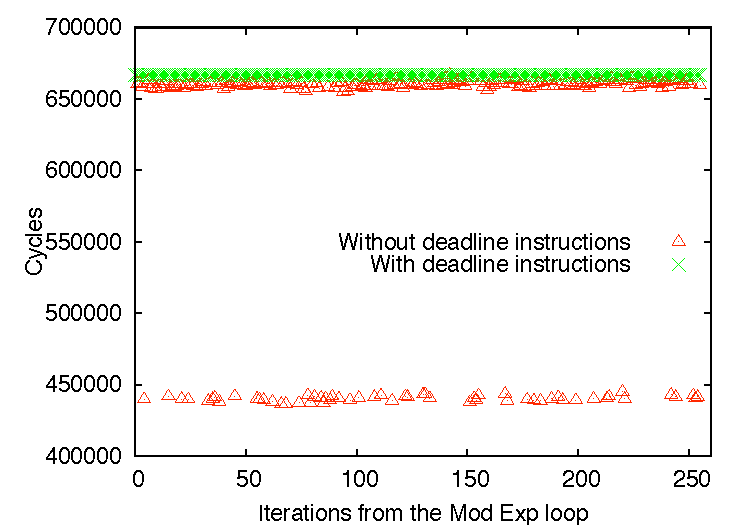
\includegraphics[width=0.48\textwidth]{./figs/RTencrypt/ModExp.pdf}
  \label{fig:modexp}
}
%\quad
\subfigure[Run time of RSA operation]{
  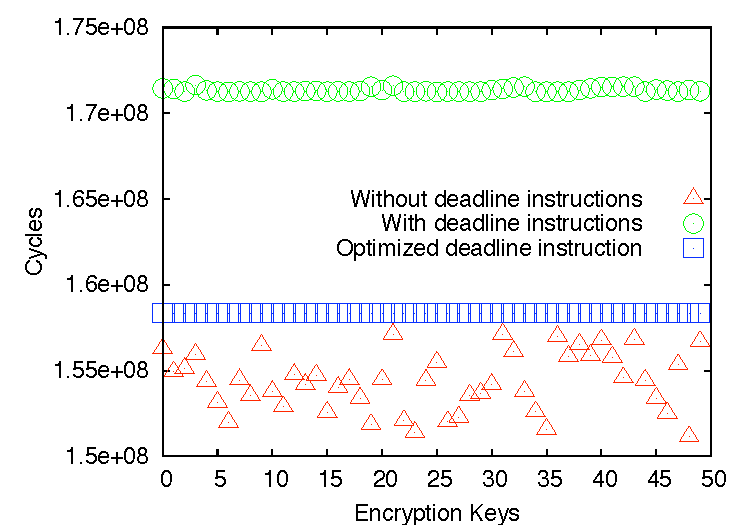
\includegraphics[width=0.48\textwidth]{./figs/RTencrypt/RSA.pdf}
  \label{fig:rsa}
}
\caption{RSA Algorithm}
\end{figure*}



%We see that all iterations took exactly the same amount of time. 
%These results seem obvious, but reveal the power of software-controlled execution time. 
%Now algorithms that require constant run time can easily be specified in software.  
%Additionally, placing deadline instructions in this loop completely eliminates the vulnerability mentioned in Kocher's\cite{Kocher96timingattacks} classic timing attack paper. 
We observe the large-scale effect of this small change on the whole encryption in figure~\ref{fig:rsa}, where RSA was run fifty times using randomly generated keys.
Without the deadline instructions (triangle points), different keys exhibit significant diversity in algorithm execution time.  
With the deadline instructions added within the modular exponentiation loop (circle points), the fluctuation is dramatically reduced to almost none. 
The remaining small variations result from code that is outside of the modular exponentiation loop, which is not influenced by the actual key.
From figure ~\ref{fig:rsa} we can see that this small variation  is not significant enough to correlate the total execution time and the key.  

% Although it seems we could have achieved a similar effect if we simply forced the algorithm to carry out the extra operation every iteration, there is a subtle difference.
% As mentioned in~\cite{Kocher96timingattacks}, always carrying out the extra multiplication operation does not make the implementation run at constant time, and timing characteristics from the squaring operation can still be exploited. 
% However, constant run time is guaranteed for code blocks enclosed within the deadline instructions, which in our case includes both the multiplication and squaring operations for each iteration.
% This simple example demonstrates the difficulty of controlling execution time using software techniques, and how straightforward it is to do so using deadline instructions. 
% This is a simple example demonstrating the concept of the deadline instruction.  
% However, for more complex algorithms, the changes required to create constant execution time might not be as obvious.
% In those situations, deadline instructions provide a straightforward mechanism to control the execution time of the algorithm.

%Although this method makes RSA secure against timing attacks, it does incur a notable performance penalty because we always run the algorithm near its worst-case execution time.
Without explicit control over timing, any attempt to make an algorithm run at constant time in software would involve manual padding of conditional branches.
This forces the algorithm to run at the worst-case execution time, similar to what we've showed.
As a result, although this makes the encryption algorithm completely secure against time-exploiting attacks, they are not adopted in practice because of this overhead.
Nevertheless, with control over execution time, we will show that running encryption algorithms in constant time does not necessarily require it to run at the absolute worst-case execution time.

%smarter techniques with deadline instructions can be used to achieve better performance while still being secure.
%Although the vulnerability is removed, readers will have noticed that an overhead was induced in this simple example. 
%The reason for the overhead is apparent, and mentioned above. 
% This overhead is not a result of the deadline instruction itself. 
% When we added the deadline instructions to the inner most loop of the modular exponentiation, in order to completely remove the vulnerability from RSA, we set the execution time of each loop iteration to always equal the execution time as if the extra operation was carried out. 
% As a result, the overall execution time will be the worst case execution time of the algorithm, as if our key was all bits of 1. 
% That is the overhead we see in figure~\ref{fig:rsa}. 
% This solution is effectively the same as timing equalization \textcolor{red}{(FIXME: add citation [do we really need one? or is this where a paper that talks about what timing equalization is would go?])} of algorithms, which now require little effort because timing can be controlled in software. 
\subsubsection{An Improved Technique of using Deadline Instructions} 
\begin{wrapfigure}[16]{r}{.45\textwidth}
%\begin{SCfigure}
\vspace{-5mm}
  \centering
  \includegraphics[scale=.60]{./figs/RTencrypt/Distro.pdf}
  \caption{Run time distribution of 1000 randomly generated keys for RSA}
  \label{fig:distro}
%\end{SCfigure}
\end{wrapfigure}

It is expected that the distribution of RSA run times will be normal over the set of all possible keys~\cite{Kocher96timingattacks}. 
Figure~\ref{fig:distro} shows the run time distribution measured for one thousand randomly generated keys. 
A curve fitting yields  a bell shaped curve formed from the run time distribution of all keys.
This means that the execution time of approximately 95\% of the keys will be within $\pm$2 standard deviations of the mean, and the worst-case execution time will be an outlier on the far right of this curve. 
Our previous example fixed the execution time of all keys to be \textit{roughly} at this far right outlier.
An improved technique capitalizes on this distribution of run times to improve performance.

First, instead of enclosing the loop iterations of the modular exponentiation operation, we enclose the whole RSA operation with deadline instructions. 
Now the deadline instructions are used to control the overall execution time of the RSA operation.
Note that we could have done this for the previous example as well to fix the execution time to be \textit{exactly} the worst-case, always. 

For RSA, key lengths typically need to be longer than $512$ bits to be considered cryptographically strong~\cite{redhatadminguide}. 
This gives roughly $2^{512}$ possible keys, which is far more than needed for most applications.
Suppose we are able reduce the key space the application covers --
instead of using $100\%$ of the keys, we refine our encryption system to only assign $97\%$ of all possible keys. Namely, the subset of keys whose RSA execution times fall on the left of the $+2$ standard deviation line on the curve.
Statistically, the keys that lie outside of $\pm 2$ standard deviation are the least secure keys anyway, since it is easier for time-exploiting attacks to distinguish those keys. 
%Then, we can reduce the value specified in the deadline instruction enclosing the whole RSA operation instead of using the absolute worst-case execution time pushed up by the far right outlier.
By doing so, we reduce the execution time of the encryption algorithm because we know that keys that are right-side outliers will not be used. 

With timing control in software, we can take advantage of this information by simply reducing the value specified in the deadline instructions enclosing the whole RSA operation. 
The square points in figure~\ref{fig:rsa} show the results of using deadline instructions in this way. 
We re-ran the same fifty keys from the previous section, and enclosed the whole operation with deadline instructions that specified the run time at +2 standard deviations from the bell curve we obtained.
We can see that, compared to the previous results that fixed the execution time of each key to take  the worst-case time (circle points), we clearly reduced the overhead while still running in constant time. 
By taking the run time difference between executions with and without deadline instructions, we obtained the overhead introduced for each of the keys with run time below 2 standard deviations (97.9\% of keys in our case) within the one thousand key set in our experiment. 
This calculation reveals that by merely reducing the key space by 3\%, running the encryption with optimized deadline instructions only introduced an average overhead of $2.3\%$ over all the keys we measured. 
All this while still being completely immune to time-exploiting attacks.
This is virtually impossible to achieve without explicit timing control, which illustrates the value of decoupling timing control and functional properties of software. 

%When running on PRET, we measured an average overhead of $11\%$ over the one thousand keys in the when we controlled the execution time of each iteration within the modular exponentiation operation.


\begin{figure*}[h]
\centering
\subfigure[Distribution of 1000 DSA keys ] {
  \includegraphics[width=0.48\textwidth]{./figs/RTencrypt/DSA_Distro.pdf}
  \label{fig:dsamodexp}
}
%\quad
\subfigure[Run time of 100 DSA operations]{
  \includegraphics[width=0.48\textwidth]{./figs/RTencrypt/DSA.pdf}
  \label{fig:dsa}
}
\caption{Digital Signature Standard Algorithm}
\end{figure*}

\subsubsection{Digital Signature Algorithm}
Kocher's~\cite{Kocher96timingattacks} original paper mentioned that Digital Signature Standard~\cite{dss} is also susceptible to timing attacks. 
Thus, to further illustrate our case, we ported the Digital Signature Algorithm from the current OpenSSL library (0.9.8j) onto PRET.
We used the same method mentioned above to secure this implementation on PRET.
Figure~\ref{fig:dsamodexp} shows the distribution of DSA run time for one thousand keys. It also shows a normal distribution.
Then, we randomly generated another one hundred keys, and measured the run time with and without deadline instructions, which we show in figure~\ref{fig:dsa}.
We can see clearly that the run time with deadline instructions is constant, and any time-exploiting attack is not possible. 

%we can set different values for the deadline instruction depending on the application's needs to yield a balance between security and performance. 
% Another possible use of deadline instructions is to implement execution time blinding. 
% We can set the execution time  of the encryption operation to be a truly random value between $\pm$2 standard deviations of the total run time. 
% Whenever the value of the deadline instruction is less the actual run time of the algorithm, the algorithm will take its normal execution time. 
% However, if the value of the deadline instruction is more than the run time, then the algorithm will run at the time specified by the deadline instruction. 
% Since the deadline instruction value is random, it detaches the correlation between the key and the run time of the encryption. 
% This can also improve the average performance.

%Simply by running on PRET, RSA is not only immune to cache attacks and branch predictor attacks, both of which can be significant dangers to RSA\cite{branchpredict,Percival05cachemissing}, but also to potential unknown timing attacks targeting the unpredictability of the architecture. 

Currently, we do not know of any work that correlates the key value with run time for different encryption algorithms. 
However, with the ability to control execution time in software, such a study would be extremely valuable.
Figures~\ref{fig:distro} and~\ref{fig:dsamodexp} show that RSA and DSA follow a normal distribution.  
Thus, from the algorithm, we postulate that by simply counting the $1$ bits in the key should be sufficient to distinguish the $95\%$ of secure keys before assigning. 
Note that no change to the encryption algorithm itself is needed, but only the key assignment process.
Since we can adjust the execution time in software, we can tune the performance of each application based on the application size, key bit length and performance needs.
All this can be done while maintaining complete immunity against time-exploiting attacks.

Note that there are several other software techniques specific to encryption algorithms that successfully defend against timing attacks. 
Our work does not lessen or replace the significance of those findings.
Instead, we can use traditional noise injection defenses on PRET as well.
For example, if reducing the key space is not possible for some applications running RSA then RSA with blinding can be ran on PRET. 
By simply running on PRET, the encryption algorithm is also secure against shared hardware resource attacks such as caches, and branch predictors. 
Other encryption algorithms that do not have software techniques or solutions readily available to counteract timing attacks can easily use the deadline instructions provided by PRET to achieve security against timing attacks.

% \section{Future Work}
% While a deadline instruction set for the worst case execution time bestows complete immunity to timing attacks, it also places overhead on virtually every execution, which may be substantial depending on the application.  Lowering the minimum time, even randomly, gives some information to an attacker, especially if there is no limitation on the number of executions the attacker may observe.  A mathematical examination of the risk involved in a reduced execution time would enable the programmer to decide what tradeoff of risk and execution delay was appropriate for the application, or appropriate in general.  For example, reducing the potential key space to a tenth of all possibilities would most likelyside-channel be an acceptable trade for faster execution, while reducing it to a billionth of all possibilities probably would not be acceptable.

% On another note, the PRET architecture as it stands is vulnerable to power attacks.  By doing very little and drawing less power while waiting for deadlines to expire, timing attacks are basically converted into a subset of power attacks.  This is unacceptable for consumer applications such as set-top boxes, where power draw can be easily measured.  Modifying the architecture to spend energy while waiting would prevent such attacks.  Depending on the implementation of the power-draining system, it might even be extended to prevent most other power attacks as well by adding another power sink to that required for useful work.

\subsection{Conclusion and Future Work}
Side-channel attacks are a credible threat to many cryptosystems.  
They exist  not just because of a weakness in an algorithm's mathematical underpinnings, but also from information leaks in the implementation of the algorithm. %The inability to control timing properties is what directly leads to side channel attacks.
In particular, this paper targets time-exploiting attacks, and lays out a means of addressing what we consider the root cause of such attacks: the lack of \textit{controllability} over the timing information leaks.
%Although numerous efforts have been put to discovering and counteracting these attacks, it seems that only more vulnerabilities are being discovered. 
% Without secure hardware, software cannot be considered truly secure.  
% Some stopgap measures are implementable in software, but rarely are they a guaranteed fix.
%that originate from the \textit{unpredictability} of the underlying hardware architecture.
As an architecture founded on predictable timing behaviors, PRET provides timing instructions to allow timing specifications in software. 
In addition, PRET is a predictable architecture that guarantees removes timing interference through a thread-interleaved pipeline with scratchpad memories for each hardware thread, and a predictable DRAM memory controller.
This eliminates the shared states in the architecture that create uncontrollable timing interference, exploited by attackers. 
Through a combination of hardware and software techniques, PRET gives control over the timing properties of programs, which effectively eliminates time-exploiting attacks. 

We demonstrate the application of these principles to known-vulnerable implementations of RSA and DSA, and show that PRET successfully defends against time-exploiting attacks with low overhead. 
Our work does not undermine the significance of any related work, which have mostly been specific to certain attacks.
PRET does not target a specific encryption algorithm, because it can be used in combination with these partial solutions on specific encryption algorithms, as well as provide a complete defense for other encryption algorithms which are less researched upon.

Besides time-exploiting attacks, there are other side-channel attacks that are legitimate threats to encryption algorithms such as power, and fault attacks.
We plan to continue to investigate PRET's effectiveness in defending against them. 
We conjecture that the thread-interleaved pipeline used in PRET can potentially help defend against power attacks because the power measured from the processor now includes significant interference from the execution of other hardware threads in the architecture.  
%Currently, PRET is only implemented as a software simulator, but as PRET moves to FPGA implementations, we can further evaluate its effectiveness in defending against power attacks.
%If our conjecture is correct, then PRET with fault tolerant techniques could potentially be a complete solution against several major side-channel attacks.  

\chapter{Related Work}
\label{chapter:related}
\label{sec:related_arch_mod}
We are certainly not the first or only one to tackle the unpredictability of computer architecture designs.
In this chapter we survey an abundance of related research to our goal of predictable architectures.
Timing analysis techniques, compiler techniques and architectural techniques all play a role in tackling the unpredictability of computer architectures.
However, we limit the scope of this survey to mainly focus on architectural techniques, as that is the focus of this thesis. 
Adding temporal semantics to programming languages has been the focus of many research proposals, but to the best of our knowledge, we believe this is the first attempt to introduce temporal semantics down at the ISA level. 

%FIXME: Compare to XMOS style handling of interrupts?

\section{Pipeline-Focused Techniques}
\subsection{Static Branch Predictors}
\label{sec:RTBranch}
Dynamic branch predictors cause timing anomalies~\cite{Engblom2003dynbranch}, and they are difficult to model because of the \textit{aliasing} of branch points.   
\textit{Aliasing} occurs when two different branches occupy the same branch predictor slot and cause interference.
Burguiere et al.~\cite{Burguiere2005staticbranchpredict} make a case for \textit{static branch prediction} to be used for real-time systems.
This can be done in several ways. 
The simplest form can predict all branches taken or not taken. 
Improvements can include the \textit{Backward Taken, Forward Not Taken} scheme, to improve performance for loops and if statements.
This scheme uses the observation that for loop control branches, almost all backwards branches are taken to return to the loop; only at the end of the loop are forward branches taken. 
With architecture support for static branch predictions, compilers can analyze code patterns (loops, if-then-else, if then) and insert instruction set constructs to denote the static prediction of each branch.  
The underlying architecture will use that for its prediction, instead of relying on a dynamic hardware unit.
This removes \textit{aliasing} and gives better estimated worst case branch mispredicts. 

Bodin et al.~\cite{Bodin2005staticbranch} use this idea of software static branch prediction to improve the WCET of programs.
Intuitively, they aim to remove all branch mispredict penalties from the worst-case path to improve the WCET. 
They propose an algorithm that iterates through the control flow graph to find the worst-case execution path (WCEP). 
Initially, the algorithm finds the worst case path assuming all the branches are mispredicted. 
Then, the algorithm assigns the static branch prediction of all branches on the WCEP to be taken.
The algorithm then iterates again to find the new WCEP until two iterations yield the same WCEP.
Since the algorithm never reassigns assigned branches, it always converges but is not optimal.
The presence of caches can easily effect the WCEP, and each branch prediction reassigned can modify the cache state.
However, the experiments assumed all code and data fit into the caches, thus the effects of caches were not factored into the algorithm.

\subsection{Superscalar Pipelines}
\label{sec:RTSuperscale}
Superscalar pipelines issue multiple instructions at a time to exploit instruction-level parallelism (ILP). 
In order to keep the pipeline filled, superscalar pipelines typically employ more aggressive techniques to fully utilize the ILP. 
As a result, attempting to model all advanced techniques often leads to either very pessimistic results, or almost infeasible complex models.

Rochange et al.~\cite{Rochange2005superscalar} propose to use instruction pre-scheduling to ease the difficulties of analysis of superscalar pipelines.  
The concept is similar to resetting the pipeline state before each basic block execution. 
This is done by postponing the scheduling of instructions from the next basic block until the instructions from the previous basic block are completed.
If it is possible to remove all timing interference across basic blocks, then the resources needed to model the pipeline can be significantly reduced, as each basic block will start with a consistent initial state.
However, the results assume the absence of caches, which can easily effect execution across basic blocks.  
Furthermore, depending on how many instructions can be in flight at one time, waiting for the pipeline state to be flushed can induce large penalties for programs with a lot of control flow transfer and small basic blocks. 

% \paragraph{A time-predictable execution mode for superscalar pipelines with instruction prescheduling ~\cite{Rochange2005superscalar}}
% \begin{itemize}
% \item What is the background of this work? What is the motivation?\\
% 
% \item What is the main goal?\\
%   They want to reconcile high performance with time
%   predictability. Mainly, they are making out of order superscalar
%   pipelines fit WCET estimation techniques. 
% \item What did they do to achieve this goal?\\
%   They control instruction flow to remove dependence between basic
%   blocks so that any WCET estimation tool would only need to measure
%   or estimate a smaller segment of code.  
% \item How do they evaluate their approach? Does it achieve the goal?
%   Do they compare it with other work?\\
%   They showed a performance comparison of slow down compared to
%   regular out of order superscalar and also against in order scalar
%   pipeline to show performance improvement. 
% \item What other work is listed as future work?\\
% \end{itemize}
% Additional questions:
% \begin{itemize}
%   \item What are the limitations/assumptions of this work?\\
%     They ignore peripheral components (cache memories, TLBs) as well
%     as external events (interrupts) and interactions with the
%     operating system (process scheduling, virtual memory, etc).
%   \item Which parts of a system/design process are modified by this
%     work? (e.g. hardware (which feature?), WCET analysis, scheduling,
%     compiler, programming language, \ldots)\\
% \end{itemize}


% \paragraph{Predictable Out-of-order Execution Using Virtual Traces ~\cite{whitham:08:predOOOwithVirtualTraces}}
% \begin{itemize}
% \item What is the background of this work? What is the motivation?\\
%   The motivation is to improve WCET of complex processors,
%   specifically for out-of-order superscalar pipelines. 
% \item What is the main goal?\\
%   The main goal of this paper is 3 fold. 1) minimizing the pessimism
%   introduced in WCET analysis. 2) increasing CPU throughput that can
%   be guaranteed. 3) minimize CPU modeling cost. 
% \item What did they do to achieve this goal?\\
%   They introduced a VTC (virtual trace controller) to control the
%   progress of the pipeline. They argue that this controller can be
%   used for a CPU of arbitrary complexity. The VTC operates CPU
%   programs as a collection of traces. Traces are paths through the
%   program. Essentially traces are formed by statically predicting
%   branches, in the context of this paper they predict the branches
%   towards the worst case execution path. This way the pipeline
%   optimizations (out of order execution etc) can optimize the worst
%   case path. This achieves goal 2, which is increased the guaranteed
%   throughput. The traces are formed via static branch predictions, and
%   the VTC contains a VTR (virtual trace register) which stores the
%   branch predictions. The pipeline state is reset between traces, so
%   the WCET analysis can be limited to within traces. The side exits
%   are determined by branch mispredicts. Now WCET within each trace and
%   side exit can be measured, and it will be the same execution time,
%   thus no CPU modeling cost is needed. This achieves goals 1 and 3. 
% \item How do they evaluate their approach? Does it achieve the goal?
%   They use the Malardalen WCET benchmark suite, but assume that
%   benchmark programs are single-path programs. They assume using IPET
%   or methods can find the WCET. They use the benchmark programs and
%   run the program on an idealized in order machine to compare the
%   results with their machine. They compare the speed up /slow down and
%   use it to analyze the issues with their approach. 
% \item What other work is listed as future work?\\
% \end{itemize}
% Additional questions:
% \begin{itemize}
%   \item What are the limitations/assumptions of this work?\\
%     They assume WCEP is easily obtained. It also depends on how many
%     traces are formed, and how effective the traces are formed. They
%     assume scratchpads in this work.
%   \item Which parts of a system/design process are modified by this
%     work? (e.g. hardware (which feature?), WCET analysis, scheduling,
%     compiler, programming language, \ldots)\\
%     They need a compiler to compile code into traces and form
%     traces. The hardware is modified with a VTC to control the traces
%     and stall the pipeline between traces. 
% \end{itemize}


Whitham et al. \cite{whitham:08:predOOOwithVirtualTraces} combine the techniques of instruction pre-scheduling and static branch predictions to propose modifications to an out-of-order superscalar pipeline to provide predictability for single thread execution.  
Instead of basic blocks, the superscalar pipeline pre-schedules instructions across \emph{virtual traces}\cite{Whitham2008formvirtualtraces}. 
\emph{Virtual traces} are program paths with static branch predictions inserted. 
These are usually formed by predicting along the WCEP, similar to the algorithm introduced by Bodin et al~\cite{Bodin2005staticbranch}. 
Each virtual trace can contain a fixed number of branches. 
A VTC (virtual trace controller) is introduced to control the progress of the pipeline.
The VTC contains a VTR (virtual trace register) which stores the branch predictions.
The pipeline state is reset between traces so the WCET analysis can be limited to within traces.
The out-of-order superscalar pipeline is also modified to disallow memory prediction and reordering of branches.
The architecture employs scratchpads instead of caches.  
This allows the execution of traces to run predictably for each different exit (branch mispredict) within a trace.
The architecture shows an improved throughput for most programs when compared to a simple in-order CPU model.
%The authors further present the effects of trace sizes to balance the main path execution time against the costs of side exits. 

% There are issues with this work, as the assumption is the ability to find the WCEP when doing the trace scheduling (how do you obtain numbers for the basic blocks with Out of Order execution, and what if program itself is so complex that the analysis is nearly infeasible?). 
% But the idea of using static branch prediction in combination with WCET could be leveraged. 
% The delayed scheduling of traces to flush the pipeline could be a huge penalty for programs with small tasks that execute frequently. 
% Reducing this delay is thus a trade off between performance of traces vs amount of state to keep to obtain the performance.

\subsection{VLIW architectures}
\label{sec:RTVLIW}
VLIW machines, like superscalars, issue multiple instructions at a time to exploit ILP.
However, unlike superscalars, VLIW machines rely on the compiler to utilize ILP and determine the instructions issued.  
This helps in the predictability because the hardware does almost no reordering or stalling.
 
Yan et al.~\cite{Yan2008VLIW} study the predictability of VLIW machines, and propose changes to the architecture and compiler to improve the predictability. 
They find that although most of the data dependency is scheduled away by the compiler, there are still several factors that limit the predictability on the hardware. 
First, since statically it is not known whether a memory access is a hit or a miss, the hardware still needs to check for it and stall when needed. 
Second, data dependencies still exist across compilation units, so the hardware still needs to support basic data dependency checking to handle those dependencies.
A compilation unit could be a basic block, a loop, a procedure or a region~\cite{Hank:1995:RCI:225160.225189}. 
Finally, if the VLIW machine uses branch prediction, there is still the need for the handling of mispredictions.

As VLIW machines heavily utilize the compiler to improve performance, they propose several compiler techniques to compile programs that lend themselves to better WCET. 
First, they use the single-path paradigm proposed by Puschner and Burns~\cite{Puschner:2002:WTP:882515.885528}, and eliminate all non-loop backwards branches with full if-conversions~\cite{Allen:1983:CCD:567067.567085}.  
To mitigate the performance penalty of single-path programming, aggressive hyperblock scheduling~\cite{Mahlke:1992:ECS:144953.144998} is used to exploit the ILP from VLIW architectures. 
For the data dependencies across compilation units, they use code padding to ensure the execution time is consistent across different paths.    
This will enable easier WCET analysis. 
This work minimally deals with instruction caches, but does not account for the effects of data cache. 

\subsection{Multithreaded Pipelines}
\subsubsection{Thread Scheduling}
With explicit hardware multithreading, the scheduling policy plays a huge role in the predictability of the architecture.
Kreuzinger et al.~\cite{Kreuzinger2000RTmultithread} evaluate the use of different real time scheduling schemes to schedule hardware threads to handle external events. 
They evaluate fixed priority preemptive (FPP), earliest deadline first (EDF), least laxity first (LLF) and guaranteed percentage (GP), which is similar to time sharing the pipeline. 
The architecture used for evaluation is a Java multi-threaded superscalar pipeline with four threads~\cite{Kreuzinger2003multithreadeventhandle}. 
A hardware priority manager is implemented to facilitate the scheduling of threads. 
All real-time threads register their real-time requirements during initialization with the priority manager. 
When the external event occurs, the priority manager schedules the corresponding interrupt service thread, and starts assigning priorities based upon the real time requirements. 
The evaluation criteria to compare scheduling policies is the throughput of the processor. 
The conclusion of the report is that in order to maximize multiple threads on a superscalar machine, the scheduler should try to keep as many threads active as long as possible to leverage thread level parallelism and hide more latencies of pipeline stalls. 
Thus GP does the best because it schedules different active threads each cycle until their percentage runs out.
Thus, it keeps threads alive as long as possible. 
The idea of using hardware threads to service interrupts is novel because of the low overhead to switch contexts. 
By giving the interrupt service routine thread priorities, it may be possible the bound the execution time of higher priority threads. 
Although the dynamic thread scheduling can cause execution time bounds to be imprecise from the effects of timing interference across threads.  
  
El-Haj-Mahmoud et al.~\cite{El-Haj-Mahmoud2005VirtualMultiprocessor} propose a statically scheduled multithreaded architecture called the Real-Time Virtual Multiprocessor (RVMP).   
The idea of a virtual processor is a slice of time on the processor. 
The RVMP extends an in-order 4-way superscalar processor to support the partitioning of the pipeline in \emph{space} and \emph{time}.  
In the \emph{space} dimension, the resources of the superscalar can be partitioned to different threads. 
In the \emph{time} dimension, the superscalar resources are time shared, and different threads are scheduled to utilize the resources at different times.  
The hardware extensions to the superscalar pipeline prevent interference between the virtual partitionings.
Scratchpads are employed for predictable memory access latencies, although they assume all accesses go to the scratchpad. 
It is unclear how accesses to shared resources, in particular main memory are dealt with.
A static round-based schedule of the thread execution is constructed to account for the real-time requirements of each thread.
The static schedule utilizes the flexibility of the different time and space partitioning options to allow threads with higher utilization more access to the pipeline. 

\subsubsection{Simultaneous Multithreaded Architectures} 
\label{sec:RTSMT}
Simultaneous Multithreaded Architectures (SMT) attempt to exploit both instruction-level and thread-level parallelism by dynamically scheduling multiple hardware threads onto a multi-way pipeline. 
In each cycle, instructions from different threads can be fetched simultaneously to fully utilize the pipeline.
The dynamic scheduling and aggressive speculation techniques render SMTs almost impossible to use for real-time systems.  
However, several proposals involve slight modifications to architecture to create a \emph{WCET-aware} SMT to be used for real-time systems.  

Barre et al.~\cite{Barre2008RTSMT} propose to assign one explicit hardware thread with the highest priority. 
That thread, called the real-time thread, gains access to any resource whenever it is scheduled. 
Any other thread that is currently occupying the resource will be preempted, and later replayed when the real-time thread is not using it.
The modifications to the SMT include additions to allow the preemption, and also the partitioning of any resource that needs to be shared. 
This gives the highest priority thread the illusion that it has the whole superscalar pipeline to itself, reducing the execution time analysis of the real-time thread to the equivalent of a superscalar architecture. 
Currently the cache effects and branch prediction are listed as future work.  

Hily et al.~\cite{Hily1999} show that out-of-order execution may not be as cost effective as in-order execution on SMT machines.
Thus, Uhrig et al.~\cite{SaschaUhrig2005SMT} propose a similar concept to Barre et al.~\cite{Barre2008RTSMT}, except for an in-order executed superscalar.
Mische et al.\cite{Mische2008SMT} expand this to allow more than one real-time thread to run on the SMT architecture.
This is done by time-sharing the highest priority thread slot among the real-time threads.  
The time-sharing schedule is statically constructed to ensure that the real-time threads still provide reasonable WCET guarantees. 
This architecture uses instruction scratchpads without data scratchpads, and no branch predictors, as the branch penalty can be filled with executions from other threads.   
Some issues do arise with the contention of memory access, as it is difficult to partition memory accesses between hardware threads.
Contention between the high priority thread slot and other thread slots are resolved by alerting the memory controller from earlier stages in the pipeline that a high priority thread will issue a memory instruction. 
This way the memory controller can hold off service to the lower priority memory accesses and wait for the high priority access to come.     
However, it is unclear how contention between the real-time threads on the high priority thread slot is resolved.
 
% \bigskip
% Although real time SMT proposals have a lot of compelling features, it
% still lacks a formal WCET analysis. All of the proposals have just
% used measured benchmarks to prove performance, and assumed that
% because the high priority thread runs as if no other thread is
% running, so static analysis is possible. In reality, WCET for a
% superscalar processor already contains pessimistic results. Although
% the lack of a branch predictor and in order execution may aid in
% this. Also, in this line of work still only one explicit hardware
% thread slot gets real-time performance, while the other threads'
% performance will have a non-continuous penalty, which is hard to
% categorize. 

\subsubsection{Thread Interleaved Pipelines}
Thread-interleaved pipelines have been proposed and employed in various architectures from research and industry. 
Besides the CDC6600~\cite{CDC6600}, described in section~\ref{section:pret_thread_pipeline}, Lee and Messerschmitt~\cite{lee1987pip}, the Denelcore HEP~\cite{HEP}, the XMOS XS1 architecture~\cite{xmos_xs1}, the Parallex Propeller chip~\cite{parallex} and the Sandbridge Sandblaster~\cite{Erdem02multi-threadedprocessor} all use fine grained thread interleaving for different applications. 
In particular, Lee and Messerschmitt~\cite{lee1987pip} and the Sandbridge Sandblaster~\cite{Erdem02multi-threadedprocessor} propose the use of thread-interleaved pipelines for DSP applications. Lee and Messerschmitt~\cite{lee1987pip} also use a round robin thread scheduling policy while the Sandblaster uses a Token Triggered Threading policy. 
The Token Triggered Threading policy is similar to the round robin scheduling policy in that each hardware thread context can only issue one instruction each in a scheduling cycle. 
However, a token is used to determine which thread's instruction is executed next. 
The XMOS XS1 architecture~\cite{xmos_xs1} allows hardware threads to dynamically be added and removed from the thread scheduling.
They use the dynamically added threads to handle interrupts, which improves the interrupt response latency. 
The XS1 architecture specifies that during execution, there will always be a minimum the number of threads equal to the pipeline depth. 
As explained in section~\ref{section:pret_thread_pipeline}, this removes pipeline hazards to improve throughput.
However, the dynamic thread scheduling can cause each thread's execution frequency to vary depending on the number of threads executing at one time.         

\subsection{Others}
\subsubsection{Virtual Simple Architecture}
Anantaraman et al.~\cite{Anantaraman2003VISA} propose the virtual simple architecture (VISA), which uses dynamic checking to ensure tasks are meeting the deadlines. 
The microarchitecture is split into two modes. 
A simple mode, which conforms to the timing of a hypothetical simple pipeline that is amenable to safe and tight WCET analysis. 
And a high performance mode, in which the architecture can use arbitrary performance-enhancing features.
A task that executes on the VISA is divided into multiple sub-tasks to gauge progress on the complex pipeline.
Each sub-task is assigned an interim deadline, based on the hypothetical simple pipeline.  
When tasks are executing on the VISA, they are first speculatively executed in high-performance mode.
If no checkpoints are missed, then the high performance mode has met the timing requirements. 
If a checkpoint is missed, the architectures switches to a simple mode to bound the remaining task times in attempt to meet the timing constraints.
The results show that the high performance mode have average executions times of 3 to 4 times faster than the simple mode.
The authors also discuss possible power savings by scaling the voltage in high performance mode.
However, the tasks and programs must have sufficient slack time to allow for dynamic checking of deadlines, and it is unclear whether the simple mode will always be able to make up the time if the high performance mode misses its checkpoint. 

\subsubsection{Java Optimized Processor}
\label{sec:RTJava}
Schoeberl presents the Java Optimized Processor (JOP)~\cite{jop:wcet} which uses Java for real time embedded systems. 
The design of JOP includes a two level stack cache architecture ~\cite{jop:stack}. 
Instead of using a large register file to store the stack, like the PicoJava\cite{McGhan1998PicoJava}, it uses only two registers to store the top two entries of the stack (Register A and Register B). 
Leveraging the stack based architecture of JavaVM, whenever an arithmetic operation occurs, the result is always stored back to the top of the stack (Register A). 
Any push or pop operation simply results in a shift of values between the two registers and the stack cache, which only requires one read and one write port for the memory. 
This architecture does not have any data hazards and has very few pipeline stages (no need for an explicit commit/writeback stage). 
Because of the few pipeline stages, it only has a small branch delay penalty, so no branch predictor is used.
All bytecode on JOP is translated into a fixed length microcode. 
Each microcode executes in a fixed number of cycles, independent of its surrounding instruction.
Thus, the WCET analysis only requires a lookup table of bytecode translated into microcode, rendering it a predictable architecture. 

\subsubsection{MCGREP}
Whitham introduces the Microprogrammed Coarse Grained Reconfigurable Processor (MCGREP)~\cite{whitam:06:mcgrep}, which is a reconfigurable predictable architecture.
The architecture of MCGREP contains multiple execution units, but each operation is implemented in microcode. 
The pipeline architecture is extremely simple, reassembling a two stage pipeline with a fetch/decode stage and an execute stage.
No internal state is stored in the pipeline, and instructions do not affect each other's execution time. 
A fast internal RAM without cache is used to store the program and used as memory for data.    
The microcode operations are predictable in the MCGREP architecture, taking a fixed number of cycles to complete.
Advanced operations can be dynamically loaded as new microcode, which enables application specific instructions to improve performance.
All MCGREP instructions take a fixed number of clock cycles to complete and are unaffected by execution history, making MCGREP a predictable processor. 

\subsubsection{ARPRET}
Andalam et al.~\cite{pretc} introduce the Auckland Reactive PRET (ARPRET) architecture to execute a new language called precision timed C (PRET-C).
PRET-C is a synchronous language extension to C designed to support synchronous concurrency, preemption, and a high-level construct for logical time.
ARPRET extends the Microblaze~\cite{xilinx-microblaze} with a custom Predictable Functional Unit (PFU) that is used for thread scheduling.
The Microblaze is configured to use on-chip memory to achieve predictable memory access latencies. 
The PFU stores the thread contexts of each thread, including the PC, thread status, priority, etc. that are used during each context switch.
By doing the thread scheduling in hardware, ARPRET reduces the thread switching overhead. 
Each thread switch is triggered in software by the C language extensions in PRET-C, and the PFU is used to determine the next context to run.   
Their benchmarks show that the ARPRET achieves predictable execution without sacrificing throughput. 
% \subsubsection{PRET}
% Craven et. al~\cite{Craven_PRET_implementation_2010}  implements PRET thread interleaved pipeline as an open source core using OpenFire 

\section{Memory-Focused Techniques}
\subsection{Caches}
The dynamic behavior of caches cause headaches for real-time systems when trying to predict memory access latencies.
Reineke et al.~\cite{Reineke07TimingPredictability} presented a study on the predictability of different cache replacement policies.
They evaluate the Least Recently Used (LRU), First In First Out (FIFO), Pseudo LRU (PLRU) and Most Recently Used (MRU) replacement policies to determine if LRU was more predictable than other policies, as observed by Heckmann et al.~\cite{Heckmann2003processor}.    
The results confirm that the LRU replacement policy was significantly more predictable than other policies.
Thus, the authors recommend any real-time system with caches to use LRU for its replacement policy. 
This paper also reveals potential for improvement in existing analyses of PLRU and FIFO.

Puat and Decotigny~\cite{Puaut02} propose to use partitioned and lock caches to eliminate the intra- and inter-task interferences when a cache is used. 
Intra-task interferences occur when different memory blocks of the same task compete for cache blocks.
Inter-task interferences occur when a preempting task's memory blocks cause cache reloads in the preempted task.
By using cache partitioning, a part of the cache is reserved for a particular task, and inter-task interference is eliminated.
To eliminate intra-task interference, cache locking is used to lock the contents of cache.
The cache contents can be locked statically, which are fixed at system start for the whole run time, or dynamically, where the contents may change.   
By locking and partitioning caches, the memory access latencies will have more predictable behavior. 

Schoeberl~\cite{jop:jtres_cache} propose to use method caches for the instruction cache of the JOP architecture~\cite{jop:wcet}.
Conventional caches use a cache line as its basic unit of replacement. 
Method caches use \emph{methods} as its unit of replacement. 
A cache can contain different block sizes that are used to store methods. 
There exists a tradeoff between performance and predictability for the block sizes of the method cache. 
Methods can occupy more than one block, depending on the method size. 
When a method is called, the cache loads the whole method into the cache, occupying any number of blocks it needs.
The LRU replacement policy is used, since the end of a method usually returns to its parent method. 
When a method is evicted, all blocks it occupies are evicted. 
Thus, the instruction cache is more predictable, because it only changes on method calls. 
Within a method, all instructions are known to be in the cache, so no cache miss results from the instruction cache.
 
%method cache SMT
Metzlaff et al.~\cite{Metzlaff2008MethodcacheSMIT} use a method cache mechanism with the real-time SMT architecture in ~\cite{Mische2008SMT}.
They partition the scratchpad for each different thread so no inter-thread interference will exist.   
Then, they implement the method cache~\cite{Kirner2007ModelFunctionCache} with scratchpads, and give priority to the high priority thread when a filling is needed.
They called this the function scratchpad.  
If the thread is stalled when a method is being filled into the scratchpad, other threads occupy the pipeline, so throughput is preserved with multiple threads. 

\subsection{Scratchpads}
Scratchpads are known to allow more precise WCET analysis~\cite{Wehmeyer2005SPM} because the contents are managed in software. 
Puaut et al.~\cite{Puaut2007SPMvsCache} present a comparison of locked caches and scratchpads, and show only subtle differences between the two in terms of performance. 
Most benchmarks give similar WCET estimates. 
The difference stems from the granularity of allocation units. 
For locked caches, the basic allocation unit is a cache line. 
Thus, it is possible to \emph{pollute} the contents of the cache line with contents that are not part of the allocation scheme. 
Also, depending on the associativity of the cache, a cache line that should be locked could possibly be in conflict with another cache line that is also locked, and thus lose its ability to be locked in the cache. 
For scratchpads, the basic allocation unit is only determined by the allocation scheme, so the contents cannot be polluted. 
However, if the basic allocation block is big, it is possible that the allocation block will not fit in the scratchpad at the end due to fragmentation.  
 
% 
% \bigskip
% \textbf{Preemption} - Although scratchpads are more predictable, the
% hardware replacement policy of caches could be advantageous,
% especially for systems that have preemption of tasks. Locked caches
% can lock content in the cache, and when a preemption occurs, the
% hardware can still take advantage of a hardware replacement for lines
% that aren't locked, while still maintaining a certain amount of
% predictability when the original task resumes (because of the locked
% content that aren't replaced). For statically allocated scratchpads,
% the allocation scheme needs to take into account the preempted task,
% and allocate space for that task. This will reduce the available
% allocation space for all other tasks. For dynamically scheduled
% schemes, it will be extremely difficult to find reload points to
% adjust the scratchpad. If a preempted task loads its optimal content
% when it preempts a task, it's unclear what to load back for the
% original task, and when to load it. There needs to be some sort of OS
% that keeps track of what was loaded off the scratchpad. It is unclear
% what overhead this could result in. (\textcolor{red}{Read papers about
%   this} \JR{Write paper about how to do this ;-)})
% 

% Scratchpad (SPM) memories provide time-predictable accesses for data.  
% However, the time-predictable SPM allocation strategies for data only support statically allocated data or stack data.  
% Dynamic data, on the other hand, is only supported by non time-predictable allocation schemes if whole-program pointer analysis identifies every memory operation that could access each variable.
 
Whitham and Audsley~\cite{whitham:09:timepredLoadStore} introduce a hardware scratchpad memory management unit (SPMMU) that manages the transfers of data between memory and the data scratchpad to eliminate \emph{pointer aliasing} and \emph{pointer invalidation}.
\emph{Pointer aliasing} occurs when the same memory location is referenced using different names (pointers). 
\emph{Pointer invalidation} occurs when an object in a memory location is moved out from that memory location.  
As a result, an alias that points to the object before the move, ends up pointing to an incorrect object.
They propose to separate \emph{logical addresses} (used by the program) and \emph{physical addresses} (identifying where an object resides).  
The SPMMU maintains a table mapping the logical address and physical address.   
Although the SPMMU resides in hardware, its contents are controlled by software via explicit OPEN and CLOSE commands in the code.  
The user specifies the base address for the object, the size of the object and the physical address at which the object is being loaded to. 
The SMMU then performs the transfer, and updates an internal table mapping the logical address to the new physical location of the object.  
This simplifies analysis because it eliminates the need for whole-pointer analysis in the program. 

% \paragraph{Implementing Time-Predictable Load and Store Operations~\cite{whitham:09:timepredLoadStore} }
% 
% \begin{itemize}
% \item Basic definitions: \\
% \textbf{Pointer aliasing:} The same memory location may be referenced using different names (pointers). 
% \textbf{Pointer invalidation:} An object in a memory location is moved out from that memory location.  As a result, an alias that points to the object before the move, ends up pointing to an incorrect object. 
% \textbf{Whole-program Pointer analysis:} Determine which pointers can point to which variables and storage locations in the entire program.
% \item What is the background of this work? What is the motivation?\\
% Scratchpad (SPM) memories provide time-predictable accesses for data.  However, the time-predictable SPM allocation strategies for data only support statically allocated data or stack data.  Dynamic data, on the other hand, is only supported by non time-predictable allocation schemes if whole-program pointer analysis identifies every memory operation that could access each variable. 
% \item What is the main goal? \\
% The objective of this paper is to implement a scratchpad memory management unit that transfers data between external memory and scratchpad memories such that pointer aliasing and pointer invalidation are eliminated. 
% This approach lifts some of the restrictions (i.e. eliminate pointers entirely from program code or no support for dynamic data) forced by the limitations of WCET analysis. 
% \item What did they do to achieve this goal?\\
% They implemented a scratchpad memory management unit (SPMMU) in hardware that performs a mapping from logical addresses (used by the program) to physical addresses (identifying where an object resides).  In addition, the SPMMU performed DMA transfers between the external memory and SPM.  The program dictates when the transfers take place via explicit OPEN and CLOSE commands in the code. The user specifies the base address for the object, the size of the object and the physical address at which the object is being loaded to.  The SMMU then performs the transfer but updates an internal table mapping the logical address to the new physical location of the object.  
% \item How do they evaluate their approach? Does it achieve the goal? Do they compare it with other work?\\
% They use three approaches to evaluate their work.  
% Their first approach simply looks at the hardware cost incurred.  In particular, they observe that since the mapping must take place in the same cycle that the request is made, it must be implemented as combinational logic; hence, a part of the critical path.  They determine this critical path and its effect on the clock frequency. 
% The second approach compares their approach for a particular function of a JPEG decode algorithm with a data cache with estimated access latencies.  They show that the SMMU is not as effective as a data cache in ideal conditions, they are much better in the worst case. 
% The third approach is a case-study implementation of the entire JPEG decode algorithm with the SMMU. 
% \item What other work is listed as future work?
% Integrating one of the SPM allocation techniques with the SMMU to determine the where to place OPEN and CLOSE commands. 
% \end{itemize}
% Additional questions:
% \begin{itemize}
%   \item What are the limitations/assumptions of this work?\\
% The user must specify the size of the object and the physical address. 
% They claim that there are algorithms that determine the best physical address, but I haven't read that work yet. 
%   \item Which parts of a system/design process are modified by this work? (e.g. hardware (which feature?), WCET analysis, scheduling, compiler, programming language, \ldots)\\
% They require the following modifications: 1) hardware, 2) WCET analysis, and 3) compilers to generate the OPEN/CLOSE commands. 
% \end{itemize}

% \subsubsection{Static allocation schemes}
% \label{sec:SPM_static_allocation}
% Static allocation schemes allocate the content on the scratchpad a
% priori, and the content stays the same throughout the whole
% execution. Most static scratchpad allocation schemes
% (\textcolor{red}{Find some citations}) use some sort of heuristic to
% find the most commonly executed instructions or data structures, and
% then allocate them statically on the scratchpad to improve the ACET
% (average case execution time). Suhendra et
% al.~\cite{Suhendra2005WCETSPM} (Abhik Roychoudhury) was the first to
% propose using static data scratchpad allocation to improve the worst
% case execution time. They first identified the difficulty in
% constructing such an algorithm that optimally allocates data to
% improve the WCET because once data is allocated on the SPM, the worst
% case execution path will change. Also, it's possible that the WCEP
% that's resulted from static analysis is actually infeasible, so the
% detection of infeasible task is also needed. As a result, they
% proposed a greedy method that allocates contents of the SPM in attempt
% to reduce the WCET. They first assume that no allocation is done for
% any memory location. They find the WCEP, and allocate the most used
% data block (not too sure of what size, does it depend on the data
% structure? Is it fixed size?)  from that path onto the SPM, then
% reiterates the algorithm to find the new WCEP. This iterates until the
% SPM space is exhausted. Note that is is sub-optimal because allocated
% content will not be reconsidered. This means that if the first WCEP
% and the second WCEP don't share that data structure, the first
% allocation does not contribute to improving the WCEP.
% 
% Patel et al.~\cite{Patel2008PRETSPM} proposed another static
% allocation scheme based on \cite{Suhendra2005WCETSPM}, except that the
% allocation criteria wasn't to minimize the WCET, but to meet all
% deadlines in the program. The greedy approach worked by synthesizing
% timing constructs (deadline blocks) into test programs. The algorithm
% works by identifying the deadline blocks that miss their
% deadline. Then a profile is constructed based on the number of
% accesses to a data block in the missed deadline blocks. Based on the
% profile, a data block is selected to be allocate on the scratchpad,
% and then the algorithm reiterates itself, until either all deadlines
% can be guaranteed to be met, or if the SPM exhausts its space. In the
% first case, the remaining space can be optimized by another method. In
% the second case, the program is deemed un-schedulable, and the
% deadlines cannot be met. 

\subsection{DRAM}
DRAM cells leak charge and have to be refreshed periodically to retain their state.
However, the refreshes of DRAMs stall other DRAM accesses, and potentially close DRAM rows, which require additional precharges to reopen them.
This causes DRAMs to be unpredictable for real-time systems, as the DRAM refreshes are usually controlled in hardware. 
Bhat and Muller~\cite{Bhat2010PredictableDRAM} tackle this specific issue of DRAM refreshes by scheduling burst refreshes.
They account for the DRAM refresh requirements in software, and schedule refresh tasks to handle the DRAM refreshes predictably. 
Two implementations are provided. 
The first is a pure software implementation, and use RAS-only refreshes to manually refresh the DRAM rows during the refresh task. 
The second implementation uses a hybrid software-hardware solution, where the software initiates a hardware DRAM refresh. 
Depending on the application needs, each refresh can contain smaller bursts at the cost of scheduling more refreshes. 
By scheduling the DRAM refresh, other DRAM accesses are more predictable because no conflict will arise from refreshes.  

Akesson et al.~\cite{Akesson2007CODES,Akesson2009DSD,Akesson2010} introduce the Predator, a predictable SDRAM memory controller. 
It is predictable by providing a guaranteed maximum latency and minimum bandwidth to each client, independent of the behavior of other clients. 
Standard DDR2 SDRAM memory controllers schedule the requests of the different components dynamically. 
Predicting the execution time of a particular component in such a system is difficult, because of interference on the shared DRAM resource. 
Predator is a hybrid between static and dynamic memory controllers.
Predator precomputes a set of of read and write groups with corresponding static sequences of SDRAM commands.
These static sequences allow the computing of latency bounds, and are scheduled by the backend dynamically. 
As predictor is meant to service multiple clients, requests by different clients are scheduled using a Credit-Controlled Static-Priority arbiter (CCSP). 
This provides a maximum latency and bandwidth to the clients based upon the guarantees of the backend. 
The front-end also may delay each response by the back-end up to its worst-case bound.
This eliminates interactions between different requestors.

Paolieri et al.~\cite{Paolieri2009ESL} present the Analyzable Memory Controller (AMC), which uses a very similar approach to the Predator. 
The main difference between AMC and Predator is that the AM uses a Round-Robin (RR) arbiter, instead of a CCSP arbiter employed in Predator. 
The RR arbiter provides the same latency and bandwidth guarantees to all clients while the CCSP provides better latency guarantee for high priority tasks. 


\chapter{Conclusion and Future work}
\label{chapter:summary}
In order to improve the efficiency and scalability of the design of CPS and safety critical systems, we contend that changes must be made to conventional abstraction layers to introduce \emph{time} as a first class citizen.
In this thesis we focus on doing so for the ISA abstraction layer and below.  
We explore instruction extensions to the ARM ISA to bring temporal semantics to the program, independent of architecture implementation.  
We also present the precision timed ARM (PTARM), an implementation of a PRET machine, in order to provide a timing predictable and composable platform for deterministic execution times.  

To bring temporal semantics to the ISA abstraction layer, we present a few instruction extensions to the existing instruction set. 
The instructions operate on a platform clock that is synchronous with the execution of instructions. 
The instruction set extensions allow programmers to specify the timing properties of program segments, and to throw hardware exceptions when the timing specifications are not met.
In this way, our instruction extensions do not over constrain the temporal semantics of the ISA, and continue to allow architecture innovation to improve program performance. 
These extensions allow programmers to begin reasoning about temporal properties of the programs independent of the underlying execution platform, provided that the ISA is faithfully implemented.

The PTARM exploits thread-level parallelism for performance by employing a predictable thread-interleaved pipeline. 
This removes the unpredictability when handling pipeline hazards, and provides temporal isolation for all hardware threads within the pipeline.
PTARM uses scratchpads instead of caches to expose the memory hierarchy, which enables a simpler and more precise WCET analysis of memory accesses.  
With a bank privatized DRAM controller, PTARM provides predictable DRAM access latencies for each hardware thread, and preserves temporal isolation between the hardware threads that access the DRAM as a shared resource.
The timing predictability and composability provided by PTARM does not come at the cost of aggregate performance, as our benchmarks show an improved throughput for both the pipeline and DRAM memory controller when fully utilized.  
Although achieving full utilization requires that applications have sufficient concurrency, the deterministic architecture can better equip CPS platforms with the ability to handle the concurrency and the uncontrollable timing properties exhibited by physical processes.

We also demonstrate the benefits of a PRET machine in the context of a real-time engine fuel rail simulator and embedded security.
To simulate an engine fuel rail in real time, we implement a platform that uses multiple PTARM cores that communicate through local shared buffers. 
The predictable timing of PTARM allows us to statically verify that the timing constraints are met.  
The timing control provided by the extended ISA enables us to implement a software based low overhead time synchronized communication protocol between the hardware threads, saving the resources required to implement a full hardware interconnection system.
These features of PTARM enable us to implement a scalable solution that can simulate, in real time, a 237 node common fuel rail systems in a single Xinlinx Virtex 6 FPGA. 
In the context of embedded security, the underlying architecture implementing encryption algorithms is susceptible to timing side-channel attacks.
Attackers can exploit the uncontrollable execution time variances caused by the architecture or algorithm to derive the key. 
We implement the RSA and DSA encryption algorithms on a PRET architecture, and show that a predictable architecture with controllable timing properties in the ISA not only defends against all timing related side-channel attacks, but eliminates the root cause of them. 

We continue to investigate the several challenges and questions mentioned in this thesis.
First, we continue to explore the formalization of the timing extensions to the ISA. 
The introduction of temporal semantics in the ISA should be platform independent; our implementation in PTARM merely opens up opportunities for further experimentation and research. 
Nailing down the formal semantics of each instruction extension is key to a consistent meaning of ``time'' that is independent of the underlying hardware implementation. 
Second, we continue to experiment with how a predictable pipeline and memory controller handles external interrupts and I/O devices.     
With the plethora of complex interfaces and protocols for modern high speed I/O interactions, typical I/O controllers are implemented in hardware.
However, we envision a predictable architecture with precise timing control can enable software implementations of protocols typically implemented in hardware due to the lack of precise control over timing in software.
A software implementation can enable flexibility for different protocols and reduce design effort, leading to faster time-to-market and more feature rich designs.        
Third, we continue to explore the interfacing with a timing predictable bus or interconnect, which can be used in timing predictable multicore systems.
In our real-time engine fuel rail simulator, we show a multicore implementation with PRET architectures that uses local shared memories for communication and  a timing based synchronization communication protocol implemented in software.  
However, as communication schemes and applications get more complex, the interconnect or bus will play a more integral role in the connection and communication of multiple PRET cores.
Thus, our future work also includes predictable communication protocols across interconnects and shared buses that leverage the predictable timing of the PRET architecture.     

It is important to understand that we are not proclaiming that all dynamic behavior in systems are harmful.
However, the dynamic behavior must be controllable and predictable. 
For example, dynamically scheduling hardware threads in the architecture causes uncontrollable timing interference because the triggering of thread switches is hidden from, and cannot be explicitly controlled by, the programmer.
We argue that only by achieving predictability in the architecture and platforms can we begin to reason about more dynamic behavior in software.
With a predictable architecture and the introduction of temporal semantics in the ISA, we hope to provide a timing deterministic foundation in the lower levels of abstraction.
In doing so, we enable larger and more complex designs of cyber-physical systems to gain more precise and efficient control over the timing properties of the system.  



%backup the six stage details 
%\appendix
%\chapter{PTARM 6 stage}
%\section{PTARM 6 stage Architecture}

The pipeline of PTARM implements a thread-interleaved pipeline for the ARM instruction set.
PTARM is written in VHDL and targets Xilinx Virtex-5 Family FPGAs, thus a the design decisions made tailored the PTARM architecture towards optimizing the design for the Xilinx V5 FPGA.
It has a 32 bit datapath and consists of a six stage pipeline and can support a minimum of six threads interleaving through the pipeline.
The pipeline can be clocked up to $180MHz$ on a Virtex-5 lx110t FPGA.  
Figure~\ref{fig:ptarm_pipeline_five_stage} shows a block diagram view of the pipeline. 
The multiplexers within the pipeline have been omitted in the figure for a simplified view of the hardware components that make up the pipeline.
There contains multiple copies of the Program Counter(PC), Thread States, and Register File, which are not shown in the figure.
Most of the pipeline design follows a typical Hennesy and Patterson\todo{citation} 5 stage pipeline, but the thread interleaved pipeline also allows us to strip away the branch predictor and the data forwarding logic used to handle data-hazards.
The six stages in the pipeline are -- Fetch, Decode, Shift, Execute, Memory, Writeback.
We will briefly describe the functional blocks of each stage, and later show how most instruction types are implemented in the pipeline.  

The fetch stage of the pipeline selects the correct PC according to which thread is executing, and passes the address to instruction scratchpad.
A simple $Log(n)$ bit upcounter is used to keep track of which thread current to fetch.  
At this point we assume the source code fits entirely on the instruction scratchpad.
Later when we present the memory hierarchy of PTARM we will discuss further about the implications of larger code bases.
Once the instruction is received from the scratchpad, it goes through a register address decoder to quickly determine what bits to send to the register.
Typical RISC instruction sets such as MIPS have encoding of instruction bits where the register operands have a fixed location for all instruction types.
Thus, once the instruction is received from instruction memory, the selected bits can be propagated as addresses to the register file. 
In the ARM instruction set however, not all instruction encoding have the register addresses at the same location. 
Thus, we insert in a simple and small logic block for a quick decoding of register addresses.
%Todo: Add more description of the logic block? 

The decode stage of the pipeline consists of the pipeline controller which does the full decoding of instructions and sets the correct pipeline signals to be propagated down the pipeline. 
Typically the controller needs to know the current instructions in the pipeline to detect the possibility of pipeline hazards.
However,in a thread-interleaved pipeline, other instructions in the pipeline belong to other threads, thus the controller logic is greatly simplified. 
It simply decodes the instruction to determine the correct signals to send to the data-path and multiplexers down the pipeline. 
These signals get propagated down the pipeline stages, and they control the execution units to ensure the correct actions are taken, and signal the multiplexers to select the correct data operands.  
Because most of ARM instructions are conditionally executed, the pipeline controller also checks the condition bis to determine whether the instruction is to be executed or not.  
The PC Adder is almost just a simple adder that increments the PC. 
The only addition is instead only outputting an address incremented by four, it outputs two addresses, the PC incremented by both four and eight. 
The address calculation of ARM branch instructions add the offset to PC+8, instead of just the current PC, so we need to store the additional PC offset of eight in case of branch instructions.
The Timer logic block is a hardware counter clocked to the processor clock which is used to implement the timing instructions mentioned in chapter~\ref{chapter:programming_models}.
The Timer counts time in nanoseconds, and it's hardware logic does not reside in the decode stage. 
The time value however is latched in the decode stage as the subsequent stages use it for timer manipulation, so in figure~\ref{fig:ptarm_pipeline_five_stage} we include it in the decode stage.
We will discuss in more detail how the timing instructions are implemented later in this chapter. 

The shift stage of the pipeline is the additional stage on top of a conventional five stage pipeline. 
The ARM ISA data-processing instructions include shifter bits and even a shifter operand for data-processing register shift instructions to shift the operands before the logical or arithmetic operations.
Thus, an extra 32 bit shifter is included to shift the operands before the execution stage. 
The Load/Store Multiple Offset logic block is used to calculate the offset of load/store multiple instructions.
The load/store multiple instruction uses a 16 bit vector to represent each of the 16 general purpose registers.
The bits that are set in that bit vector represents a load/store on that register.
The an offset is added to the base memory address for the instruction, and that offset depends on how many bits are set. 
Thus, the load/store multiple offset logic block does a bit count on the bit vector and adjusts the offset to be passed into the ALU for load/store multiple instructions.
We will later describe in detail how the load/store multiple instructions are executed within the pipeline.
The timer adder logic block is a 32 bit add/subtract unit. 
Since time is represented in 64 bit values, we add an additional 32 bit add/subtract-er so the execution stage doesn't need to incorporate a 64 bit ALU.

The execute stage simply just contains the 32 bit ALU that can do both logical and arithmetic operations. 
The memory stage interacts with the data scratchpad and memory controller, and the write back stage writes the correct data back to the registers and hardware thread states.

The floating point hardware units are pipelined floating point computation units generated with the Xilinx Coregen tool. 
 
%TODO: Memory Hierarchy
\section{Instruction Implementations}
In this section we will go into more details about how each instruction type is implemented and how the hardware blocks shown in the previous sections are used.
We will go through different instruction types and also discuss the timing implications of our implementation. 
We will summarize with a table with all instructions and the cycle count it takes to execute them.   
\subsection{Data-Processing}

\subsection{Branch}
\begin{figure}
  \vspace{-20pt}
  \begin{center}
    \includegraphics[scale=.6]{figs/branch_pipeline_implementation}
  \end{center}
  \vspace{-20pt}
  \caption{Branch Instruction Execution in the Ptarm Pipeline}
  \label{fig:branch_pipeline_implementation}
\end{figure}
Branch instructions in the ARM can conditionally branch forward or backwards by up to 32MB. 
Because the general purpose register 15 is the PC, any write to R15 is also considered a branch instruction that branches to the address written into R15.
Figure~\ref{fig:branch_pipeline_implementation} show how the branch instruction is executed in the thread-interleaved pipeline. 
The hardware units involved are highlighted in gray and the lines are in bold.
The branch instructions for the ARM ISA calculate the address based upon an offset added to PC incremented by 8. 
Thus, the PC adder, in addition to incrementing the PC by 4, also increments the PC by 8 to pass to the ALU for correct address calculation. 
Once the address is calculated, it is written back to the PC for the corresponding thread.
If the instruction is a branch and link ($bl$), PC+4 will be written back to the link register (R14).   
In the case of a conditional branch, the PC is only written back if the condition holds true, or else PC+4 is written back to the PC. 
Because of the thread interleaved pipeline, we are not concerned that the pipeline will be stalled waiting for result of the branch to execute the next instruction. 
Instead, instructions from other threads will be fetched before the results of the branch is needed.     
Thus, we can write back to the PC at the end of the pipeline without creating hazards.
\subsection{Loads and Stores}
\begin{figure}
  \vspace{-20pt}
  \begin{center}
    \includegraphics[scale=.6]{figs/ldstr_pipeline_implementation}
  \end{center}
  \vspace{-20pt}
  \caption{Load/Store Instruction Execution in the Ptarm Pipeline}
  \label{fig:ldstr_pipeline_implementation}
\end{figure}
For load and store instructions, the memory access address is formed by combining a base register and an offset value. 
ARM also specifies the ability to update the base register after any memory operation. 
This compacts code that reads arrays, as a load or store instruction can access memory and updates the base register so the next memory access is done on the updated base register.
ARM calls these pre-indexed and post-indexed addressing modes. 
Pre-indexed addressing mode calculates the memory address by first using the value of the base register and offset, then updating the base register. 
Post-indexed addressing mode first updates the base register, then uses the updated base register value along with the offset to form the memory address. 
The base register could be incremented or decremented when it is being updated.   
Because there is only one write port to our register file however, we cannot simultaneously write back a load result from memory and the updated base register to the register file in a single cycle. 
As a result, 
\subsection{Floating Point}

\subsection{Timing Instructions}

\section{PTARM Simulator}
\label{sec:ptarm_sim}

\section{Worst Case Execution Time Analysis}
\label{sec:wcet}






\bibliographystyle{abbrv}
\bibliography{thesis,PretOneDCFDApp,survey,controller}  


% That's all folks!
\end{document}
